\documentclass{article}

\PassOptionsToPackage{numbers, compress}{natbib}

\usepackage{subfig}
\usepackage[utf8]{inputenc} % allow utf-8 input
\usepackage[T1]{fontenc}    % use 8-bit T1 fonts
% \usepackage{hyperref}       % hyperlinks
\usepackage{url}            % simple URL typesetting
\usepackage{booktabs}       % professional-quality tables
\usepackage{amsfonts}       % blackboard math symbols
\usepackage{nicefrac}       % compact symbols for 1/2, etc.
\usepackage{microtype}      % microtypography
\usepackage{xcolor}    
\usepackage{color, colortbl}% colors
\usepackage{algorithm}
\usepackage{algorithmic}
% \usepackage{algpseudocode}
\usepackage[pdftex]{graphicx}
\usepackage{appendix}
\usepackage{multirow}
\usepackage{amsmath}
\usepackage{comment}
\usepackage[colorlinks]{hyperref} 
\usepackage{xcolor}
\usepackage{xspace}
\usepackage{enumitem}
\usepackage[normalem]{ulem}

\renewcommand{\algorithmiccomment}[1]{\hfill $\triangleright$ #1}

\definecolor{LightCyan}{rgb}{0.88,1,1}

% hyperlinks
\hypersetup{colorlinks,allcolors=[rgb]{0.6,0.15,0.00098}}

\newcommand{\chen}[1]{{\color{cyan}{#1}}}
\newcommand{\haotian}[1]{{\color{red}{#1}}}
\newcommand{\alex}[1]{{\color{blue}{\textbf{alex}: #1}}}

\newcommand{\ie}{\textit{i.e.}\xspace}
\newcommand{\eg}{\textit{e.g.}\xspace}
\DeclareMathOperator*{\argmax}{arg\,max}
\DeclareMathOperator*{\argmin}{arg\,min}

% if you need to pass options to natbib, use, e.g.:
%     \PassOptionsToPackage{numbers, compress}{natbib}
% before loading neurips_2023


% ready for submission
\usepackage[final]{neurips_2024}


% to compile a preprint version, e.g., for submission to arXiv, add add the
% [preprint] option:
%     \usepackage[preprint]{neurips_2023}


% to compile a camera-ready version, add the [final] option, e.g.:
%     \usepackage[final]{neurips_2023}


% to avoid loading the natbib package, add option nonatbib:
%    \usepackage[nonatbib]{neurips_2023}


\usepackage[utf8]{inputenc} % allow utf-8 input
\usepackage[T1]{fontenc}    % use 8-bit T1 fonts
\usepackage{hyperref}       % hyperlinks
\usepackage{url}            % simple URL typesetting
\usepackage{booktabs}       % professional-quality tables
\usepackage{amsfonts}       % blackboard math symbols
\usepackage{nicefrac}       % compact symbols for 1/2, etc.
\usepackage{microtype}      % microtypography
\usepackage{xcolor}         % colors



\title{Pixel is a Barrier: Diffusion Models Are More Adversarially Robust Than We Think}


% The \author macro works with any number of authors. There are two commands
% used to separate the names and addresses of multiple authors: \And and \AND.
%
% Using \And between authors leaves it to LaTeX to determine where to break the
% lines. Using \AND forces a line break at that point. So, if LaTeX puts 3 of 4
% authors names on the first line, and the last on the second line, try using
% \AND instead of \And before the third author name.


\author{%
  Haotian Xue \\
  Georgia Institute of Technology\\
  htxue.ai@gatech.edu\\
  \And
   Yongxin Chen\\
  Georgia Institute of Technology\\
  yongchen@gatech.edu\\
}


\begin{document}


\maketitle


\begin{abstract}

% Adversarial examples for diffusion models are widely used as solutions for safety concerns. By adding adversarial perturbations to personal images, attackers can not edit or imitate them easily. However, it is essential to note that all these protections target the latent diffusion model (LDMs), the adversarial examples for diffusion models in the pixel space (PDMs) are largely overlooked. This may mislead us to think that the diffusion models are vulnerable to adversarial attacks like most deep models. In this paper, we show novel findings that: even though gradient-based white-box attacks can be used to attack the LDMs, they fail to attack PDMs. This finding is supported by extensive experiments of almost a wide range of attacking methods on various PDMs and LDMs with different model structures, meaning diffusion models are much more robust against adversarial attacks. Moreover, we find that PDMs can be used as an off-the-shelf purifier to effectively remove the adversarial patterns that were generated on LDMs to protect the images, which means that most protection methods nowadays, to some extent, cannot protect our images from malicious attacks. We hope that our insights will inspire the community to rethink the adversarial samples for diffusion models as protection methods and move forward to more effective protection. Codes are available in \url{https://github.com/xavihart/PDM-Pure}.

Diffusion models have demonstrated an impressive capability to edit or imitate images, which has raised concerns regarding the safeguarding of intellectual property. To address these concerns, the adoption of adversarial attacks, which introduce adversarial perturbations into protected images, has proven successful. Consequently, diffusion models, like many other deep network models, are believed to be susceptible to adversarial attacks. However, in this work, we draw attention to an important oversight in existing research, as all previous studies have focused solely on attacking latent diffusion models (LDMs), neglecting adversarial examples for diffusion models in the pixel space (PDMs). Through extensive experiments, we demonstrate that nearly all existing adversarial attack methods designed for LDMs fail when applied to PDMs. We attribute the vulnerability of LDMs to their encoders, indicating that diffusion models exhibit strong robustness against adversarial attacks. Building upon this insight, we propose utilizing PDMs as an off-the-shelf purifier to effectively eliminate adversarial patterns generated by LDMs, thereby maintaining the integrity of images. Notably, we highlight that most existing protection methods can be easily bypassed using PDM-based purification. We hope our findings prompt a reevaluation of adversarial samples for diffusion models as potential protection methods. Codes are available in \url{https://github.com/xavihart/PDM-Pure}.


% Generative Diffusion Models excel at generating high-quality images however, they can cause safety issues by maliciously editing or mimicking 







\end{abstract}


\section{Introduction}

Generative diffusion models (DMs)~\citep{ddpm,song2020score,ldm} have achieved great success in generating images with high fidelity. However, this remarkable generative capability of diffusion models is accompanied by safety concerns~\cite{zhang2023text}, especially on the unauthorized editing or imitation of personal images such as portraits or individual artworks~\cite{andersen2023,setty2023}.
%
Recent works~\cite{advdm, glaze,salman2023raising, sdsattack, mist-v2, chen2024smoothattack,ahn2024imperceptible, metacloak} show that adversarial samples (adv-samples) for diffusion models can be applied as a protection against malicious editing. Small perturbations generated by conventional methods in adversarial machine learning~\citep{pgd,goodfellow2014fgsm} can effectively fool popular diffusion models such as Stable Diffusion~\cite{ldm} to produce chaotic results when an imitation attempt is made. However, a significantly overlooked aspect is that all the existing works focus on latent diffusion models (LDMs) and the pixel-space diffusion models (PDMs) are not studied. For LDMs, perturbations are not directly introduced to the input of the diffusion models. Instead, they are applied externally and propagated through an encoder. It has been shown that the encoder-decoder of LDMs is vulnerable to adversarial perturbations ~\cite{zhang2023robustness,sdsattack}, which means that the adv-samples for LDMs have a very different mechanism compared with the adv-samples for PDMs. 
Moreover, some existing works~\cite{liang2023mist, salman2023raising} show that combining encoder-specific loss can enhance the adversary, ~\cite{sdsattack} further demonstrating that 
% the gradient of the denoising process is weak and unstable, and 
the encoder is the bottleneck for attacking LDMs. Building upon this observation, in this paper, we draw attention to
rethink existing adversarial attack methods for diffusion models:

\begin{center}
    \textit{Can we generate adversarial examples for PDMs as we did for LDMs?}
\end{center}

% \chen{combine this with the first paragraph before raising our research question} 

% Instead of attacking the diffusion process itself, current adversarial examples for Latent Diffusion Models heavily rely on attacking the encoder: Glaze~\cite{glaze} is built on minimizing the distance between the attacked image and the target image in the latent space defined by the encoder. Additionally, Mist~\cite{liang2023mist} demonstrates the significance of combining the textural loss derived from the encoder to generate better adversarial samples. Moreover, SDS-attack \cite{sdsattack} further investigates that, the gradient of denoising process is weak and unstable, and the real bottleneck of attacking an LDM is attacking the encoder.
%

We address this question by systematically investigating adv-samples for PDMs. We conduct experiments on various LDMs or PDMs with different network architectures (e.g. U-Net~\cite{ddpm} or Transformer~\cite{dit}), different training datasets, and different input resolutions (e.g. 64, 256, 512). Through extensive experiments, we demonstrate that all the existing methods we tested ~\citep{liang2023mist,mist-v2, glaze, sdsattack, chen2024smoothattack, salman2023raising, advdm}, targeting to attack LDMs, fail to generate effective adv-samples for PDMs. This implies that PDMs are more adversarial robust than we think. 

% \chen{this is confusing More importantly, it means that the previous adversarial examples for diffusion models (AdvDM) are, in fact, one special case of adv-samples for LDMs (AdvLDM) only.}

Building on this insight that PDMs are strongly robust against adversarial perturbations, we further propose PDM-Pure, a universal purifier that can effectively remove the protective perturbations of different scales (e.g. Mist-v2~\cite{mist-v2} and Glaze~\cite{glaze}) based on PDMs trained on large datasets. Through extensive experiments, we demonstrate that PDM-Pure achieves way better performance than all baseline methods.

% \chen{no need to mention this in introduction While GrIDPure~\cite{zhao2023can} shows that we can apply diffusion models in different resolutions to purify our image patch-by-patch, they miss that the key is in fact the pixel space, not the resolution.}



% Pixel is a barrier, the original reverse process of PDMs introduces large randomness directly in the pixel space, making the whole system quite robust to be fooled to generate bad samples. Pixel is also a barrier preventing us from achieving real protection using adversarial perturbations since strong PDMs can be utilized to remove the out-of-distribution perturbations~\cite{diff-pgd}. Our work calls for attention to rethink the problem of adv-samples for DM, and also rethink whether adv-samples can protect our images. Our contributions are summarized as follows.

% \begin{enumerate}[parsep=0pt,topsep=0pt,leftmargin=12pt]
%     \item We revist adversarial examples for diffusion models by investigating PDMs, an area that has largely been overlooked in this field. Existing attacks on LDMs \textbf{can not} be applied to attack PDMs, which means that PDMs show superior robustness against adversarial perturbations.
%     \item Based on the new insights, we propose a simple but effective framework to apply strong PDMs as \textbf{a universal purifier} to remove attack-agnostic adversarial perturbations, easily bypassing current protective methods. 
%     \item \chen{is this a contribution?} We emphasize that \textbf{pixel is a barrier}, the community should rethink the adv-samples for DMs and whether current protections based on adv-samples for LDMs, really provide effective protection.
% \end{enumerate}


To summarize, the pixel is a barrier to adversarial attack; the diffusion process in the pixel space makes PDMs much more robust than LDMs. This property of PDMs also makes real protection against the misusage of diffusion models difficult since all the existing protections can be easily purified using a strong PDM. Our contributions are listed below.

\begin{enumerate}[parsep=0pt,topsep=0pt,leftmargin=12pt]
    \item We observe that most existing works on adversarial examples for protection focus on LDMs. Adversarial attacks against PDMs are \textbf{largely overlooked} in this field. 
    \item We fill in the gap in the literature by conducting extensive experiments on various LDMs and PDMs. We discover that all the existing methods \textbf{fail} to attack the PDMs, indicating that PDMs are much more adversarially robust than LDMs.
    \item Based on this novel insight, we propose a simple yet effective framework termed PDM-Pure that applies strong PDMs as \textbf{a universal purifier} to remove attack-agnostic adversarial perturbations, easily bypassing almost all existing protective methods. 

\end{enumerate}



% we made an observation that most of the works focus on LDM, PDMs are not studied

% we test it and find that PDM is much more robust than LDMs 

% PDM-Pure 




\twocolumn[{%
	\renewcommand\twocolumn[1][]{#1}%
	\maketitle
	\begin{center}
		\newcommand{\teaserwidth}{\textwidth}
		% \vspace{-0.15in}
		\centerline{
			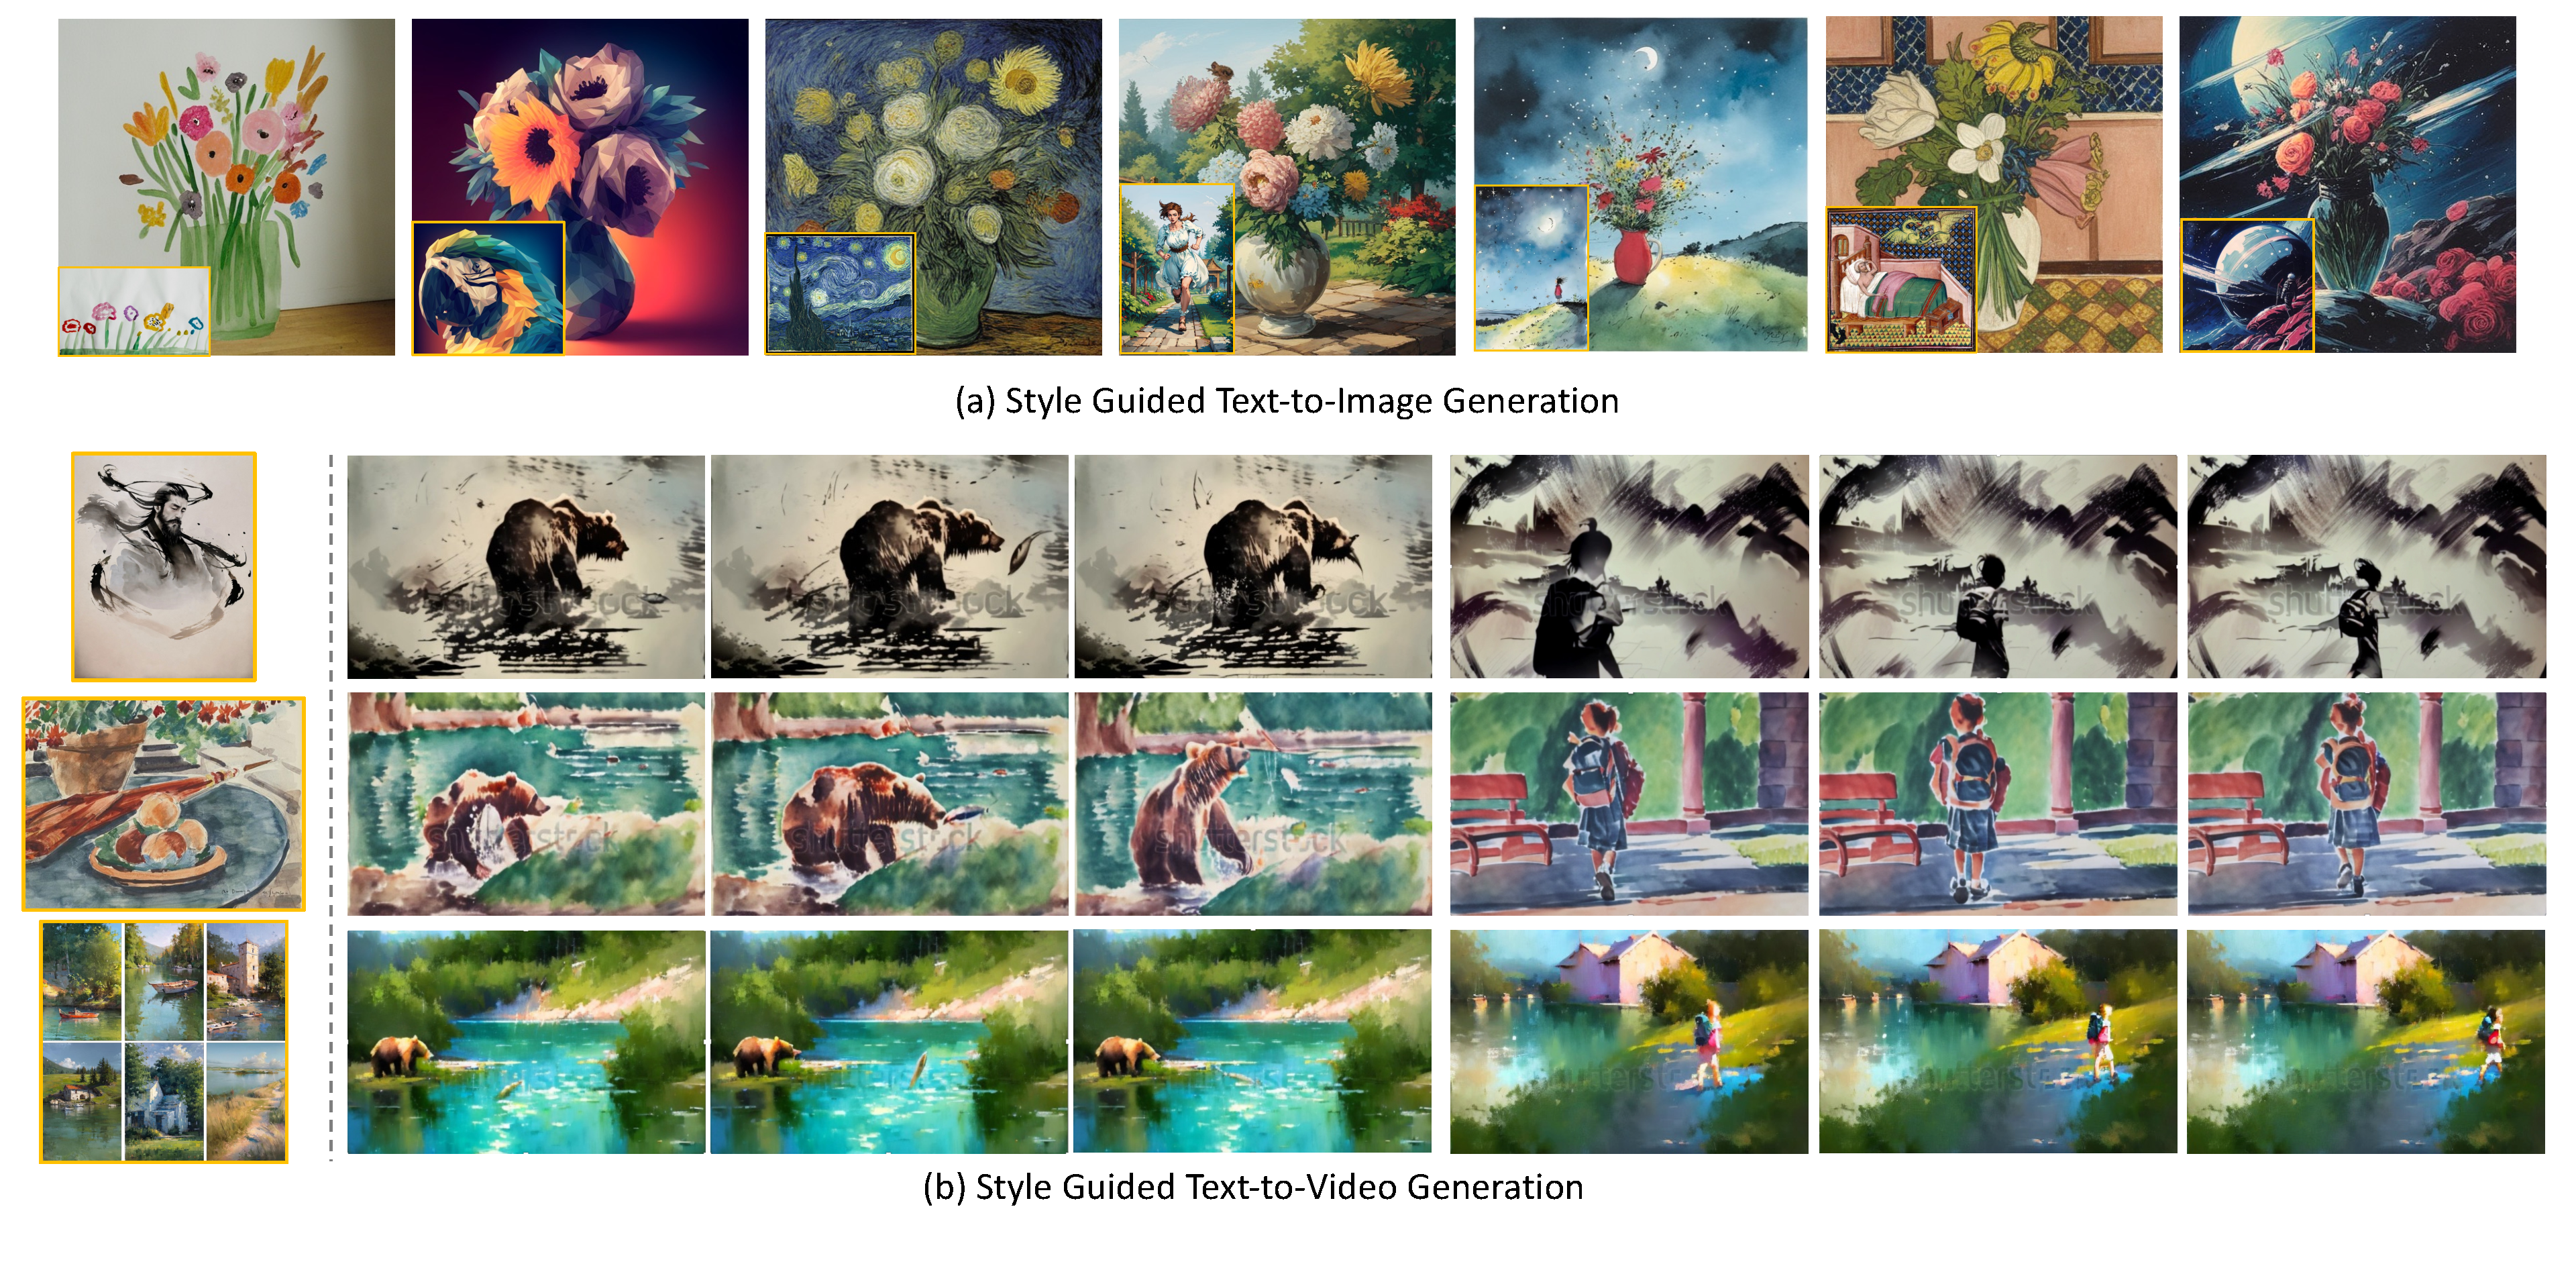
\includegraphics[width=\teaserwidth,clip]{figures/pdf_files/teaser.pdf}
		}
		\vspace{-1ex}
		\captionof{figure}{\textbf{Human Gaussian Splats (\acronym)} is a neural rendering framework that trains on 50-100 frames of a monocular video containing a human in a scene. HUGS enables novel view rendering with novel human poses at 60 FPS by learning a disentangled representation that can also render the human in other scenes. }
		% \vspace{-0.08in}
		\label{fig:teaser}
	\end{center}%
}]

% background

% issues


% what we find


%

\section{Related Works}

\paragraph{Safety Issues in Diffusion Models}
The impressive generative capability of the diffusion models has raised numerous safety issues~\cite{zhang2023text,setty2023,andersen2023}. As a result, there has been a growing interest in preventing DMs from being abused. Some of the existing works focus on the protection of intellectual property of diffusion models by applying watermarks~\citep{zhao2023recipe, peng2023protecting, cui2023diffusionshield} and some of them are on concept removal to prevent the DMs from generating NSFW images~\citep{heng2023continual,zhang2023forget,gandikota2023unified}. In the era of generative models, caution should be taken to guarantee safe and responsible applications of these models.

\paragraph{Adversarial Examples for DMs} Adversarial samples~\cite{goodfellow2014fgsm, carlini2017towards, glaze} are clean samples perturbed by an imperceptible small noise that can fool the deep neural networks into making wrong decisions. Under the white-box settings, gradient-based methods are widely used to generate adv-samples. Among them, the projected gradient descent (PGD) algorithm~\cite{pgd} is one of the most effective methods. Recent works~\citep{advdm, salman2023raising} show that it is also easy to find adv-samples for diffusion models (AdvDM): with a proper loss to attack the denoising process, the perturbed image can fool the diffusion models to generate chaotic images when operating diffusion-based mimicry. Furthermore, many improved algorithms~\cite{mist-v2,chen2024smoothattack,sdsattack} have been proposed to generate better AdvDM samples. However, to our best knowledge, all the AdvDM methods listed above are used on LDMs, and those for the PDMs are rarely explored.

\paragraph{Adversarial Perturbation as Protection} Adversarial perturbation against DMs turns out to be an effective method to safeguard images against unauthorized editing~\cite{advdm, glaze,salman2023raising, sdsattack, mist-v2, chen2024smoothattack,ahn2024imperceptible, metacloak}. It has found applications (e.g., Glaze~\cite{glaze} and Mist~\cite{mist-v2, liang2023mist}) for individual artists to protect their creations. SDS-attack~\cite{sdsattack} further investigates the mechanism behind the attack and proposes some tools to make the protection more effective. However, they are limited to protecting LDMs only.
% without further investigating whether they can work for more general PDMs. 
In addition, some works~\cite{zhao2023can, sandoval2023jpeg} find that these protective perturbations can be purified. For instance, GrIDPure~\cite{zhao2023can} find that DiffPure~\cite{nie2022diffusion} can be used to purify the adversarial patterns, but they did not realize that the reason behind this is the robustness of PDMs.


\begin{figure}[t]
  \centering
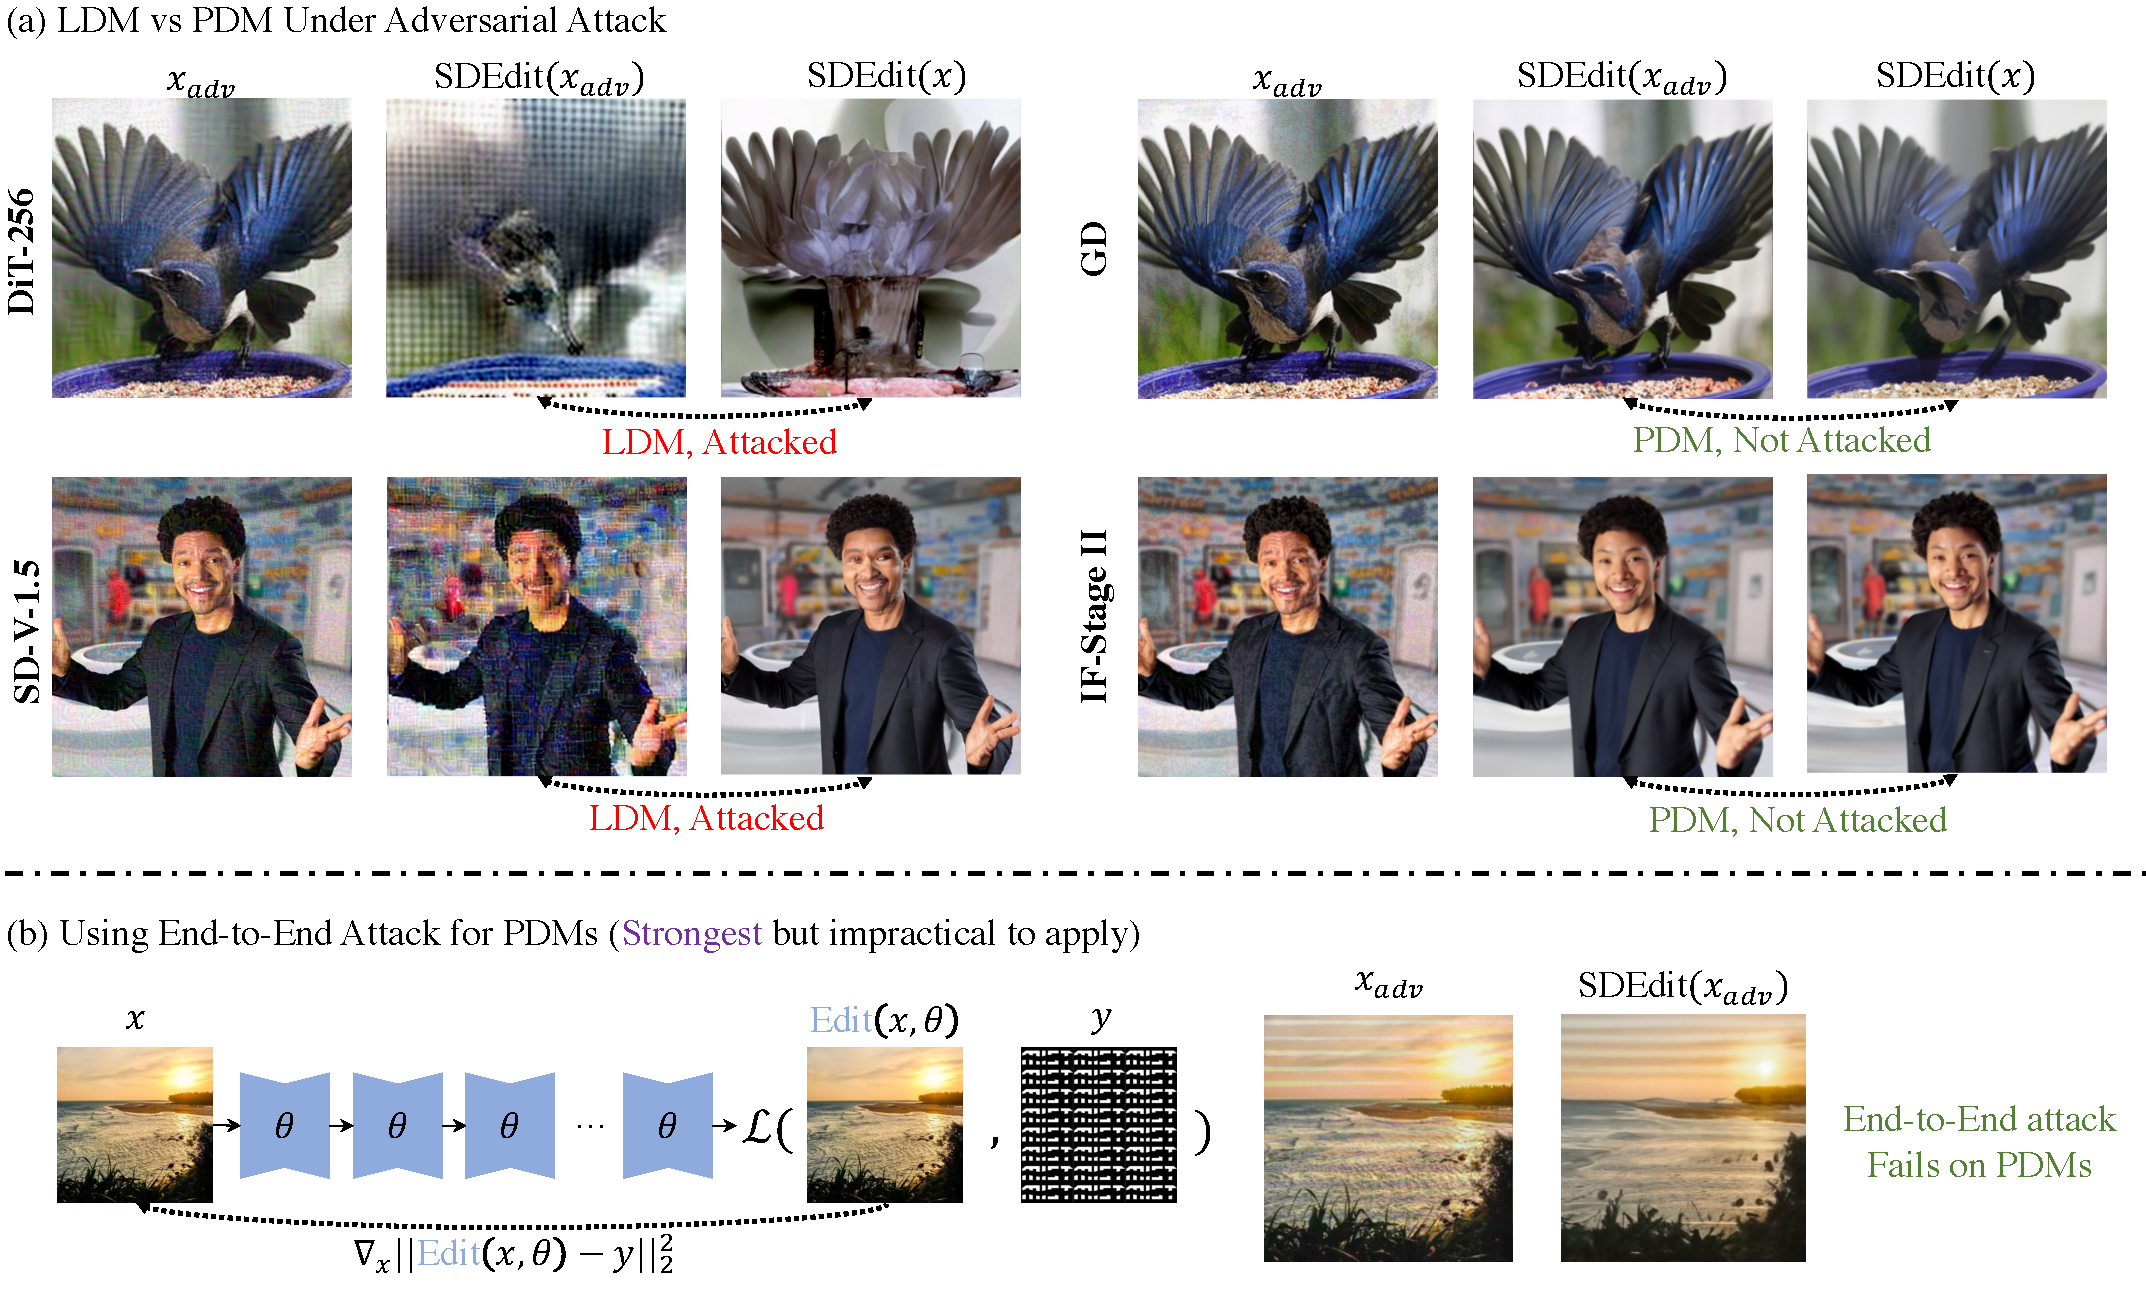
\includegraphics[width=0.99\linewidth]{images/attack.pdf}
  \caption{\textbf{PDMs Cannot be Attacked as LDMs}: (a) LDMs can be easily fooled but PDMs cannot be. (b) Even End-to-End attack does not work on PDMs. (Best viewed with zoom-in)}

  \label{fig:attack_various_models}
  \vspace{-0.4cm}
\end{figure}



\section{Preliminaries}

\paragraph{Generative Diffusion Models}

The generative diffusion model~
\cite{ddpm, song2020score} is one type of generative model, and it has demonstrated remarkable generative capability in numerous fields such as image~\cite{ldm, balaji2022ediffi}, 3D~\cite{poole2022dreamfusion, lin2022magic3d}, video~\cite{vdm,makeavideo}, story~\cite{pan2022story, rahman2023make} and music~\cite{musicdiff, huang2023noise2music} generation. Diffusion models, like other generative models, are parametrized models $p_{\theta}(\hat{x}_0)$ that can estimate an unknown distribution $q(x_0)$. For image generation tasks, $q(x_0)$ is the distribution of real images.

There are two processes involved in a diffusion model, a forward diffusion process and a reverse denoising process. The forward diffusion process progressively injects noise into the clean image, and the $t$-th step diffusion is formulated as $q(x_t \mid x_{t-1} ) = \mathcal{N} (x_t; \sqrt{1 - \beta_t}x_{t-1}, \, \beta_t \mathbf{I})$. Accumulating the noise, we have $    q_t(x_t \mid x_0 ) = \mathcal{N} (x_t; \sqrt{\bar{\alpha}_t} \, x_{t-1}, \, (1-\bar{\alpha}_t) \mathbf{I})$. Here $\beta_t$ growing from $0$ to $1$ are pre-defined values,  $\alpha_t = 1-\beta_t$, and $\bar{\alpha}_t = \Pi_{s=1}^{t} \alpha_s$. Finally, $x_T$ will become approximately an isotropic Gaussian random variable when $\bar{\alpha}_t \rightarrow 0$. 

Reversely, $p_{\theta}(\hat{x}_{t-1}|\hat{x}_{t})$ can generate samples from Gaussian $\hat{x}_T \sim\mathcal{N} (0, \textbf{I})$, where $p_{\theta}$ be re-parameterized by learning a noise estimator $\epsilon_{\theta}$, the training loss is $\mathbb{E}_{t, x_0, \epsilon}[\lambda(t)\|\epsilon_{\theta}(x_t,t) - \epsilon \|^2]$ weighted by $\lambda(t)$, where $\epsilon$ is the noise used to diffuse $x_0$ following $q_t(x_t|x_0)$. Finally, by iteratively applying $p_{\theta}(\hat{x}_{t-1}|\hat{x}_{t})$, we can sample realistic images following $p_{\theta}(\hat{x}_0)$.


Since the above diffusion process operates directly in the pixel space, we call such diffusion models Pixel-Space Diffusion Models (PDMs). Another popular choice is to move the diffusion process into the latent space to make it more scalable, resulting in the Latent Diffusion Models (LDMs)~\cite{ldm}. More specifically, LDMs first use an encoder $\mathcal{E}_{\phi}$ parameterized by $\phi$ to encode $x_0$ into a latent variable $z_0 = \mathcal{E}_{\phi}(x_0)$. The denoising diffusion process is the same as PDMs. At the end of the denoising process, $\hat{z}_0$ can be projected back to the pixel space using decoder $\mathcal{D}_{\psi}$ parameterized by $\psi$ as $\hat{x}_0 = \mathcal{D}_{\psi}(\hat{z}_0)$.

% \chen{breifly introduce SDEdit?}






\begin{table}[t]
 
  \label{tab:my_label}
 \resizebox{\textwidth}{!}{%
  \centering
  \begin{tabular}{c|ccc|ccc|ccc|ccc|c}
  \toprule
    \multicolumn{1}{c}{Models} & 
    \multicolumn{3}{c}{\textbf{FID-score}$\uparrow$} & \multicolumn{3}{c}{\textbf{SSIM} $\downarrow$} & \multicolumn{3}{c}{\textbf{LPIPS} $\uparrow$} & \multicolumn{3}{c}{\textbf{IA-Score} $\downarrow$}  & \textbf{Type} \\
    \midrule
  $\delta=4/255$ & Clean & Adv & $\Delta$  & Clean & Adv & $\Delta$  & Clean & Adv & $\Delta$ & Clean & Adv & $\Delta$ &   \\  

    \midrule
DiT-256 & 131 & 167  & {\color{red}+36}  & 0.37 & 0.35 & {\color{red}-0.02} & 0.44 & 0.54 & {\color{red}+0.10} & 0.74 & 0.70 & {\color{red}-0.04} & LDM  \\
SD-V-1.4 & 44 & 114  & {\color{red}+70}  & 0.68 & 0.55 & {\color{red}-0.13}  & 0.22 & 0.46 & {\color{red}+0.24}  & 0.92 & 0.84 & {\color{red}-0.08}  & LDM  \\
SD-V-1.5 & 45 & 113 & {\color{red}+68}  & 0.73 & 0.59 & {\color{red}-0.14} & 0.20 & 0.38 & {\color{red}+0.138} & 0.94 & 0.89 & {\color{red}-0.05} & LDM  \\
GD-ImageNet & 109 & 109  & +0  & 0.66 & 0.66 & -0.00 & 0.21 & 0.21 & +0.00 & 0.90 & 0.90 & -0.00 & PDM  \\
IF-I & 186 & 187  & +1  & 0.59 & 0.58 & -0.01 & 0.14 & 0.14 & +0.00 & 0.86 & 0.86 & -0.00 & PDM  \\
IF-II & 85 & 87  & +2 & 0.84 & 0.84 & -0.00 & 0.15 & 0.15 & +0.00 & 0.91 & 0.91 & -0.00 & PDM   \\

\midrule
  $\delta=8/255$ & Clean & Adv & $\Delta$  & Clean & Adv & $\Delta$  & Clean & Adv & $\Delta$ & Clean & Adv & $\Delta$ &   \\  

    \midrule
DiT-256 &131 & 186  &{\color{red}+55}  & 0.37 & 0.31 & {\color{red}-0.06} & 0.44 & 0.63 & {\color{red}+0.19} & 0.74 & 0.66 & {\color{red}-0.08} & LDM  \\
SD-V-1.4 & 44 & 178  & {\color{red}+134}  & 0.68 & 0.44 & {\color{red}-0.24}  & 0.22 & 0.60 & {\color{red}+0.38}  & 0.92 & 0.78 & {\color{red}-0.14}  & LDM  \\
SD-V-1.5 & 45 & 179  & {\color{red}+134}  & 0.73 & 0.49 & {\color{red}-0.24} & 0.20 & 0.51 & {\color{red}+0.31} & 0.94 & 0.84 & {\color{red}-0.10} & LDM  \\
GD-ImageNet & 109 & 110  & +1  & 0.66 & 0.64 & -0.02 & 0.21 & 0.22 & +0.01 & 0.90 & 0.90 & -0.00 & PDM  \\
IF-I & 186 & 188  & +2  & 0.59 & 0.59 & -0.00 & 0.14 & 0.14 & +0.00 & 0.86 & 0.86 & +0.00 & PDM  \\
IF-II & 85 & 82   & -3  & 0.84 & 0.83 & -0.01 & 0.15 & 0.16 & +0.01 & 0.91 & 0.92 & +0.01 & PDM   \\






\midrule
  $\delta=16/255$ & clean & adv & $\Delta$  & clean & adv & $\Delta$  & clean & adv & $\Delta$ & clean & adv & $\Delta$ &   \\  

  \midrule
DiT-256 & 131 & 220  & {\color{red}+89}  & 0.37 & 0.26 & {\color{red}-0.11} & 0.44 & 0.70 & {\color{red}+0.26} & 0.74 & 0.63 & {\color{red}-0.11} & LDM  \\
SD-V-1.4 & 44 & 225  & {\color{red}+181}  & 0.68 & 0.34 & {\color{red}-0.34}  & 0.22 & 0.68 & {\color{red}+0.46}  & 0.92 & 0.72 & {\color{red}-0.20}  & LDM  \\
SD-V-1.5 & 45 & 226  & {\color{red}+181}  & 0.73 & 0.37 & {\color{red}-0.36} & 0.20 & 0.62 & {\color{red}+0.42} & 0.94 & 0.78 & {\color{red}-0.16} & LDM  \\
GD-ImageNet & 109 & 110  & +1  & 0.66 & 0.57 & -0.09 & 0.21 & 0.26 & +0.05 & 0.90 & 0.89 & -0.01 & PDM  \\
IF-I & 186 & 188  & +2  & 0.59 & 0.58 & -0.01 & 0.14 & 0.15 & +0.01 & 0.86 & 0.87 & +0.01 & PDM  \\
IF-II &85 & 86  & +1  & 0.84 & 0.76 & -0.08 & 0.15 & 0.21 & +0.06 & 0.91 & 0.95 & +0.04 & PDM   \\


\bottomrule
  \end{tabular}
}
\vspace{10pt}
 \caption{
  \textbf{Quantiative Measurement of PGD-based Adv-Attacks for LDMs and PDMs}: gradient-based diffusion attacks can attack LDMs effectively, making the difference $\Delta$ across all evaluation metrics between edited clean image and edited adversarial image large, which means the quality of edited images drops dramatically (in red). However, the PDMs are not affected much by the crafted adversarial perturbations, showing small $\Delta$ before and after the attacks.
  }
  \label{quant_protect}
  \vspace{-20pt}
\end{table}





\paragraph{Adversarial Examples for Diffusion Models} 
Recent works~\cite{salman2023raising, advdm} find that adding small perturbations to clean images will make the diffusion models perform badly in noise prediction, and further generate chaotic results in tasks like image editing and customized generation. The adversarial perturbations for LDMs can be generated by optimizing the Monte-Carlo-based adversarial loss:

\vspace{-0.4cm}
\begin{equation}\label{semantic_loss}
        \mathcal{L}_{adv}(x) = \mathbb{E}_{t, \epsilon} \mathbb{E}_{z_t \sim q_t(\mathcal{E}_{\phi}(x))}\|\epsilon_{\theta}(z_t, t) -\epsilon \|_2^2.
\end{equation}
\vspace{-0.4cm}

Other encoder-based losses~\cite{glaze, liang2023mist, mist-v2, sdsattack} further enhance the attack to make it more effective. With the carefully designed adversarial loss, we can run Projected Gradient Descent (PGD)~\cite{pgd} with $\ell_{\infty}$ budget $\delta$ to generate adversarial perturbations: 
% \chen{make it clear that $x$ is the clean image}
% \chen{use $x^k$? also $B_\infty(x^k, \delta)$?} \haotian{should be $B_\infty(x, \delta)$, since the budget is computed on the clean sample}

\vspace{-0.4cm}
\begin{equation}\label{pgd_update}    x^{k+1} = \mathcal{P}_{B_\infty(x^0, \delta)} \left[ x^{k} + \eta\, \text{sign}\nabla_{x^k}\mathcal{L}_{adv}(x^k) \right]
\end{equation}

 In the above equation, $\mathcal{P}_{B_\infty(x^0, \delta)}(\cdot)$ is the projection operator on the $\ell_\infty$ ball, where $x^0$ is the clean image to be perturbed. We use superscript $x^k$ to represent the iterations of the PGD and subscript $x_t$ for the diffusion steps. 

    
\begin{figure}[t]
  \centering
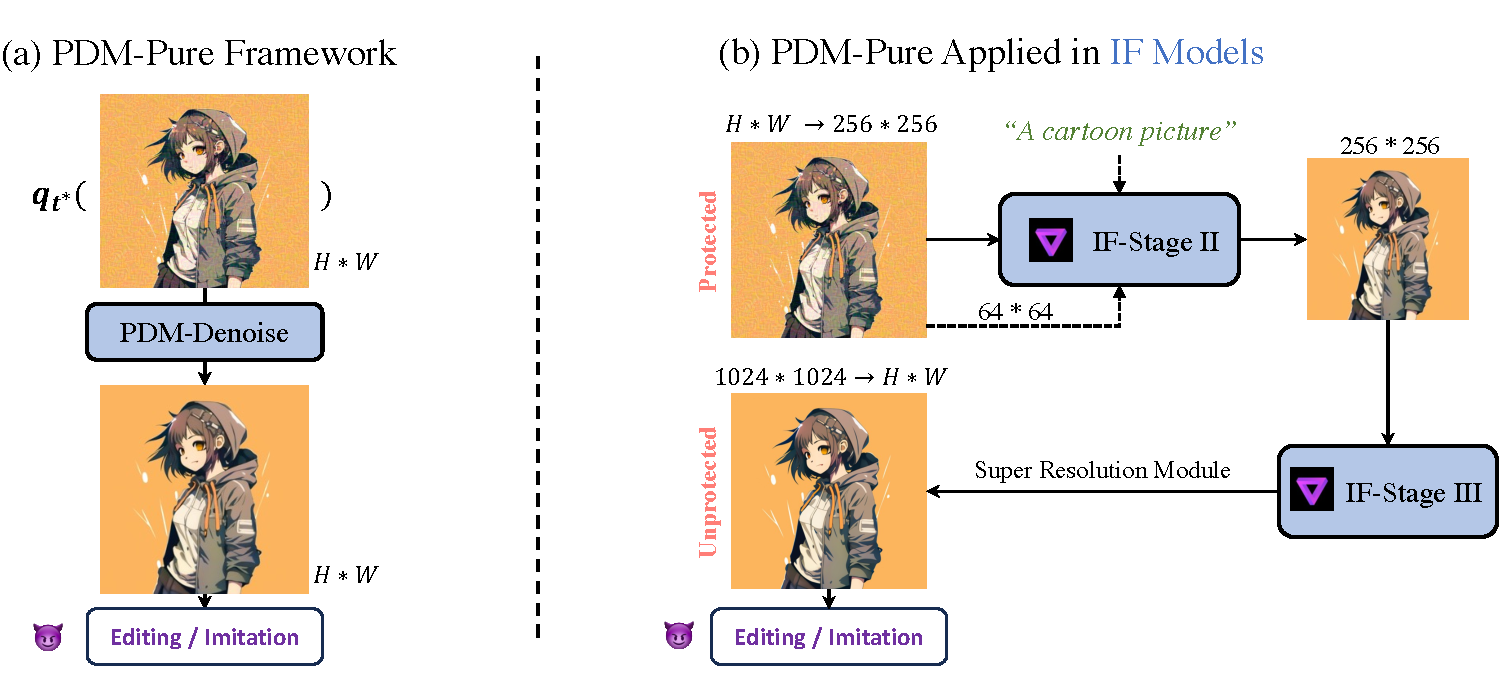
\includegraphics[width=0.8\linewidth]{images/purifier.pdf}
  \vspace{-5pt}
  \caption{\textbf{PDM-Pure is Easy to Design:} (a) PDM-Pure applies SDEdit~\cite{meng2021sdedit} in the pixel space: it first runs forward diffusion with a small step $t^{*}$ and then runs denoising process. (b) We adapt the framework to DeepFloyd-IF~\cite{deepfloyd}, one of the strongest PDMs. PDM-Pure can effectively remove strong protective perturbations (e.g. $\delta=16/255$). The images we tested are sized $512\times 512$.}

\label{fig:purification_pipeline}
  \vspace{-0.5cm}
\end{figure}



\section{Rethink Adversarial Examples for Diffusion Models}

Adversarial examples of LDMs are widely adopted as a protection mechanism to prevent unauthorized images from being edited or imitated~\cite{glaze, liang2023mist}. However, a significant issue overlooked is that all the adversarial examples in existing work are generated using LDMs, primarily due to the wide impact of the Stable Diffusion; no attempts have been made to attack PDMs. 

This lack of investigation may mislead us to conclude that diffusion models, like most deep neural networks, are vulnerable to adversarial perturbations, and that the algorithms used in LDMs can be transferred to PDMs by simply applying the same adversarial loss in the pixel space formulated as:

\vspace{-0.4cm}
\begin{equation}\label{pixel_diffusion_adversarial_loss}
    \mathcal{L}_{adv}(x) = \mathbb{E}_{t, \epsilon} \mathbb{E}_{x_t \sim q_t(x)}\|\epsilon_{\theta}(x_t, t) -\epsilon \|_2^2
\end{equation}

However, we show through experiments that PDMs are robust against this form of attack (Figure~\ref{fig:attack_various_models}), which means all the existing attacks against diffusion models are, in fact, special cases of attacks against the LDMs only.
Prior to this study, there may have been a prevailing belief that diffusion models could be easily deceived. However, our research reveals an important distinction: it is the LDMs that exhibit vulnerability, while the PDMs demonstrate significantly higher adversarial robustness.
% Before this work, people may think that diffusion models can be easily fooled, but the truth is that only LDMs are, the original PDMs are much more adversarially robust. 
We conduct extensive experiments on popular LDMs and PDMs structures including DiT, Guided Diffusion, Stable Diffusion, and DeepFloyd, and demonstrate in Table~\ref{quant_protect} that only the LDMs can be attacked and PDMs are not that susceptible to adversarial perturbations. More details and analysis can be found in the experiment section.



The vulnerability of the LDMs is caused by the vulnerability of the latent space~\cite{sdsattack}, meaning that although we may set budgets for perturbations in the pixel space, the perturbations in the latent space can be large. In~\cite{sdsattack}, the authors show statistics of perturbations in the latent space over the perturbations in the pixel space and this value $\frac{|\delta_z|}{|\delta_x|}$ can be as large as $10$. In contrast, the PDMs directly work in the pixel space, and thus the injected noise combined with the random Gaussian noise will not easily fool the denoiser as it is trained to be robust to Gaussian noise of different levels. 








Almost all the copyright protection perturbations~\cite{glaze, liang2023mist, mist-v2} are based on the insight that it is easy to craft adversarial examples to fool the diffusion models.  We need to rethink the adversarial samples of diffusion models since there are a lot of PDMs that cannot be attacked easily. Next, we show that PDMs can be utilized to purify all adversarial patterns generated by existing methods in Section~\ref{sec:pdm_pure}.  This new landscape poses new challenges to ensure the security and robustness of diffusion-based copyright protection techniques.




\section{PDM-Pure: PDM as a Strong  Universal Purifier}~\label{sec:pdm_pure}
\vspace{-0.4cm}

Given the robustness of PDMs, a natural idea emerges: we can utilize PDMs as a universal purification network. This approach could potentially eliminate any adversarial patterns without knowing the nature of the attacks. We term this framework \textbf{PDM-Pure}, which is a general framework to deal with all the perturbations nowadays. To fully harness the capabilities of PDM-Pure, we need to fulfill two basic requirements: (1) The perturbation shows out-of-distribution pattern as reflected in existing works on adversarial purification/attacks using diffusion models~\cite{nie2022diffusion,diff-pgd} (2) The PDM being used is strong enough to represent $p(x_0)$, which can be largely determined by the dataset they are trained on. 

It is \textbf{effortless} to design a PDM-Pure. The key idea behind this method is to run SDEdit in the pixel space. Given any strong pixel-space diffusion model, we add a small noise to the protected images and run the denoising process (Figure~\ref{fig:purification_pipeline}), and then the adversarial pattern should be removed. The key idea of PDM-Pure is simple. In practice, we need to adjust the pipeline to fit the resolution of the PDMs being used. 

Here, we explain in detail how to adapt DeepFloyd-IF~\cite{deepfloyd}, the strongest open-source PDM as far as we know, for PDM-Pure. DeepFloyd-IF is a cascaded text-to-image diffusion model trained on 1.2B text-image pairs from LAION dataset~\cite{schuhmann2022laion}. It contains three stages named IF-Stage I, II, and III. Here we only use Stage II and III since Stage I works in a resolution of $64$ which is too low. Given a perturbed image $x_{W\times H}$ sized $W\times H$, we first resize it into $x_{64\times 64}$ and $x_{256\times 256}$. Then we use a general prompt  $\mathcal{P}$ to do SDEdit~\cite{meng2021sdedit} using the Stage II model: 
% $x_t = \textbf{IF-II}(x_{t+1}, x_{64\times 64}, p)$

\begin{equation}
    x_t = \textbf{IF-II}(x_{t+1}, x_{64\times 64}, \mathcal{P})
\end{equation}

where $t=T_{\text{edit}}-1, ...,1, 0$, $x_{T_{\text{edit}}}=x_{256\times 256}$. A larger $T_{\text{edit}}$ may be used for larger noise. $x_0$ is the purified image we get in the $256\times 256$ resolution space, where the adversarial patterns should be already purified. We can then use IF Stage III to further up-sample it into $1024\times 1024$ with $x_{1024\times 1024} = \textbf{IF-III}(x_0, p)$. Finally, we can sample into $H\times W$ as we want through downsampling. This whole process is demonstrated in Figure~\ref{fig:purification_pipeline}. After purification, the image is no longer adversarial to the targeted diffusion models and can be effectively used in downstream tasks.

In the main paper, we conduct experiments on purifying protected images sized $512\times 512$. For images with a larger resolution, purifying in the resolution of $256\times 256$ may lose information. In Appendix~\ref{supp:section:pdm_pure_for_higher_resolution} we show PDM-Pure can also applied to purify patches of high-resolution inputs.








\begin{table}[t]
 
  \label{tab:my_label}
 \resizebox{\textwidth}{!}{%
  \centering
  \begin{tabular}{ccccccccc}
\toprule
Methods & AdvDM & AdvDM(-) & SDS(-) & SDS(+) & SDST & Photoguard & Mist & Mist-v2 \\

% \midrule

% $\delta=4/255$ \\
% \midrule

% Crop-Resize & 0 & 0 & 0 & 0 & 0 & 0 & 0 & 0\\

% JPEG & 0 & 0 & 0 & 0 & 0 & 0 & 0 & 0\\

% Adv-Clean & 0 & 0 & 0 & 0 & 0 & 0 & 0 & 0\\

% LDM-Pure& 0 & 0 & 0 & 0 & 0 & 0 & 0 & 0\\

% GrIDPure & 0 & 0 & 0 & 0 & 0 & 0 & 0 & 0\\

% PDM-Pure (ours) & 0 & 0 & 0 & 0 & 0 & 0 & 0 & 0\\

% \midrule
% $\delta=16/255$ \\
\midrule

Before Protection & 166 & 166 & 166 & 166 & 166 & 166 & 166 & 166 \\

After Protection & 297 &221 & 231 & 299 & 322 & 375 & 372 & 370 \\

\midrule

Crop-Resize & 210 & 271 & 228 & 217 & 280 & 295 & 289 & 288\\

JPEG & 296 & 222 & 229 & 297 & 320 & 359 & 351 & 348 \\

Adv-Clean & 243 & 201 & 204 & 244 & 243 & 266 & 282 & 270 \\

LDM-Pure& 300 & 251 & 235 & 300 & 350 & 385 & 380 & 375 \\

GrIDPure & 200 & 182 & 195 & 200 & 210 & 220 & 230 & 210 \\
\rowcolor{LightCyan}
PDM-Pure (ours) & \textbf{161} & \textbf{170} & \textbf{165} & \textbf{159} & \textbf{179} & \textbf{175} & \textbf{178} & \textbf{170}\\

\bottomrule
  \end{tabular}

}
\vspace{10pt}
 \caption{
  \textbf{Quantiative Measurement of Different Purification Methods in Different Scale (FID-score)}: We compute the FID-score of editing purified images over the clean dataset. PDM-Pure is the strongest to remove all the tested protection, under strong protection with $\delta=16$. GrIDPure~\cite{zhao2023can} can also do reasonable protection, but the performance is limited because the PDM they used is not strong enough.
  }
  \label{quant_purify}
  \vspace{-0.8cm}
\end{table}

\section{Experiments}

In this section, we conduct experiments on various attacking methods and various models to support the following two conclusions:

\begin{itemize}[parsep=0pt,topsep=0pt,leftmargin=12pt]
    \item \textbf{(C1)}: PDMs are much more adversarial robust than LDMs, and PDMs can not be effectively attacked using all the existing attacks for LDMs.
    \item \textbf{(C2)}: PDMs can be applied to effectively purify all of the existing protective perturbations. Our PDM-Pure based on DeepFloyd-IF shows state-of-the-art purification power.
    % \item \textbf{(C3)}: Pixel is a barrier for us to achieve real protection against diffusion-based mimicry. PDM-Pure can make the protective perturbation no more protective, and there is currently no effective way to attack PDMs.
\end{itemize}

\subsection{Models, Datasets, and Metrics} 
The models we used can be categorized into LDMs and PDMs. For LDMs, we use Stable Diffusion V-1.4, V-1.5 (SD-V-1.4, SD-V-1.5)~\cite{ldm}, and Diffusion Transformer (DiT-XL/2)~\cite{dit}, and for PDMs we use Guided Diffusion (GD)~\cite{guideddiffusion} trained on ImageNet~\cite{deng2009imagenet}, and DeepFloyd Stage I and Stage II~\cite{deepfloyd}. 

For models trained on the ImageNet (DiT, GD), we run adversarial attacks and purification on a 1k subset of the ImageNet validation dataset. For models trained on LAION, we run tests on the dataset proposed in~\cite{sdsattack}, which includes $400$ cartoon, artwork, landscape, and portrait images. The metrics for testing the quality of generated images are included in the Appendix.

For protection methods, we consider almost all the representative approaches, including AdvDM~\cite{advdm}, SDS~\cite{sdsattack}, Mist~\cite{liang2023mist}, Mist-v2~\cite{mist-v2}, Photoguard~\cite{salman2023raising} and Glaze~\cite{glaze}. We also test the methods in the design space proposed in ~\cite{sdsattack}, including  SDS(-), AdvDM(-), and SDST. In contrast to other existing methods, they are based on gradient descent and have shown great performance in deceiving the LDMs.






\subsection{(C1) PDMs are Much More Robust Than We Think} 

In Table~\ref{quant_protect}, we attack different LDMs and PDMs with one of the most popular adversarial loss~\cite{mist-v2} in Equation~\ref{semantic_loss} and Equation~\ref{pixel_diffusion_adversarial_loss}, which can be interpreted as fooling the denoiser using a Monte-Carlo-based loss. Given the attacked samples, we test the SDEdit results on the attacked samples, which can be generally used to test whether the samples are adversarial for the diffusion model or not. We use FID-score~\cite{fid}, SSIM~\cite{ssim}, LPIPS~\cite{lpips}, and IA-Score~\cite{la-score} to measure the quality of the attack. If the quality of generated images decreases a lot compared with editing the clean images, then the attack is successful. We can see that LDMs can be easily attacked, while PDMs are quite robust; the quality of the edited images is still good. We also show some visualizations in Figure~\ref{fig:attack_various_models}, which illustrates that the perturbation will affect the LDMs but not the PDMs.

To further investigate how robust PDM is, we test other advanced attacking methods, including the End-to-End Diffusion Attacks (E2E-Photoguard) proposed in~\cite{salman2023raising} and the Improved Targeted Attack (ITA) proposed in ~\cite{mist-v2}. Though the End-to-End attack is usually impractical to run, it shows the strongest performance to attack LDMs.  We find that both attacks are not successful in PDM settings. We show attacked samples and edited samples in Figure~\ref{fig:attack_various_models} as well as the Appendix. In conclusion, existing adversarial attack methods for diffusion models can only work for the LDMs, and PDMs are more robust than we think.


\subsection{(C2) PDM-Pure: A Universal Purifier that is Simple yet Effective}

PDM-Pure is simple: basically, we just run SDEdit to purify the protected image in the pixel space. Given our assumption that PDMs are quite robust, we can use PDMs trained on large-scale datasets as a universal black-box purifier. We follow the model pipeline introduced in Section~\ref{sec:pdm_pure} and purify images protected by various methods in Table~\ref{quant_purify}.

PDM-Pure is effective: from Table~\ref{quant_purify} we can see that the purification will remove adversarial patterns for all the protection methods we tested, largely decreasing the FID score for the SDEdit task. Also, we test the protected images and purified images in more tasks including Image Inpainting~\cite{song2020score}, Textual-Inversion~\cite{textualinversion}, and LoRA customization~\cite{lora} in Figure~\ref{fig:purification_results}. Both qualitative and quantitative results show that the purified images are no more adversarial and can be effectively edited or imitated in different tasks without any obstruction. 

Also, PDM-Pure shows SOTA results compared with previous purification methods, including some simple purifiers based on compression and filtering like Adv-Clean, crop-and-resize, JPEG Compression, and  SDEdit-based methods like GrIDPure~\cite{zhao2023can}, which uses patchified SDEdit with a GD~\cite{guideddiffusion}. We also add LDM-Pure as a baseline to show that LDMs can not be used to purify the protected images. For GrIDPure, we use Guided-Diffusion trained on ImageNet to run patchified purification. All the experiments are conducted on the datasets collected in ~\cite{sdsattack} under the resolution of $512\times 512$. Results for higher resolutions are presented in Appendix~\ref{supp:section:pdm_pure_for_higher_resolution}.




% \subsection{(C3) Pixel is A Barrier: What Should We Do in the Future?}

% \chen{why is this in the experiment section? Are any experiments involved?} Pixel is a barrier for us to do real protection against adversarial attacks. Since PDMs are quite robust, they cannot be easily attacked and can even be used to purify the protective perturbations, challenging the current assumption for safety protection of generative diffusion models. The community should rethink the problem of adversarial samples for generative diffusion models and rethink can we rely on them to protect unauthorized images. Hence, diffusion models turn out to be quite robust, more research should be conducted to study them and the reason behind them. If the robustness can be verified and guaranteed, we may rely on it as a new structure for many other tasks.\haotian{move it the the conclusion}


\section{Conclusions and Future Directions}


In this paper, we present novel insights that while many studies demonstrate the ease of finding adversarial samples for Latent Diffusion Models (LDMs), Pixel Diffusion Models (PDMs) exhibit far greater adversarial robustness than previously assumed. We are the first to investigate the adversarial samples for PDMs, revealing a surprising discovery that existing attacks fail to fool PDMs. Leveraging this insight, we propose utilizing strong PDMs as universal purifiers, resulting in PDM-Pure, a simple yet effective framework that can generate protective perturbations in a black-box manner. 


Pixel is a barrier for us to do
real protection against adversarial attacks. Since PDMs are quite robust, they cannot be easily attacked.
PDMs can even be used to purify the protective perturbations, challenging the current assumption for
the safe protection of generative diffusion models. We advocate rethinking the problem of
adversarial samples for generative diffusion models and 
unauthorized image protection based on it. 
% Diffusion models turn out to be quite robust, 
More rigorous study can be
conducted to better understand the mechanism behind the robustness of PDMs. Furthermore, we can utilize it as a new structure for many other tasks

\begin{figure}[H]
  \centering
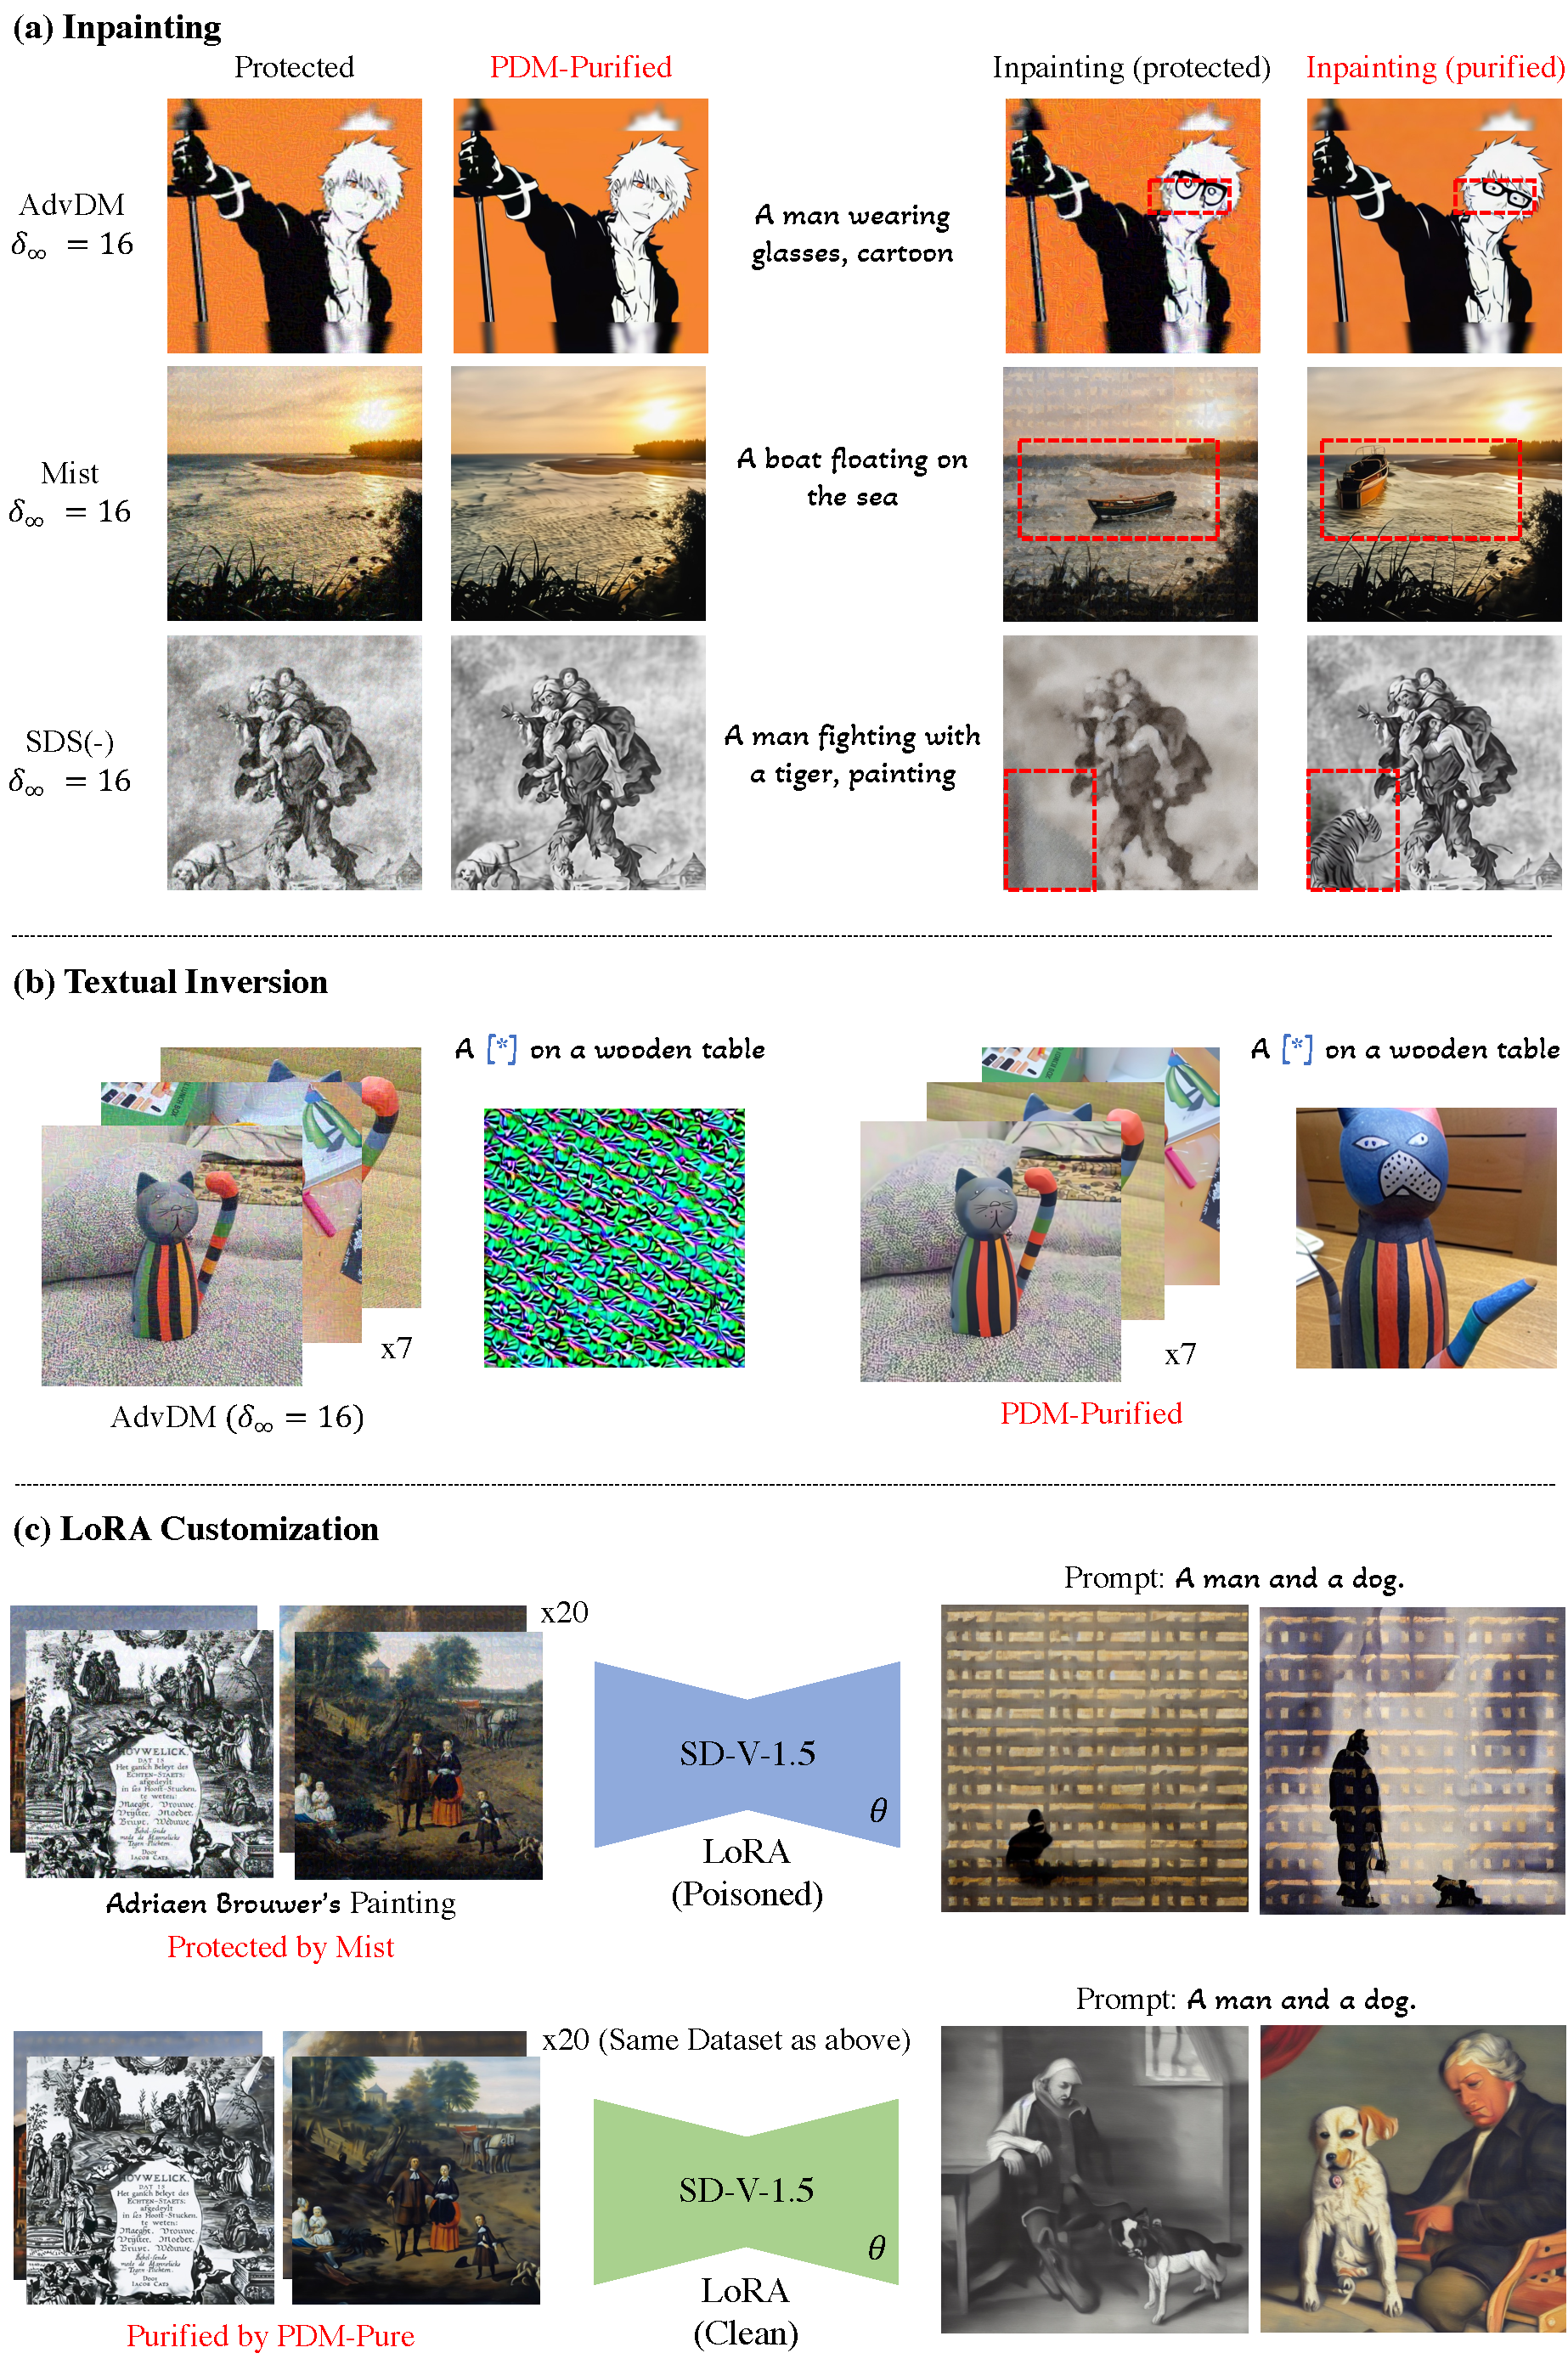
\includegraphics[width=0.99\linewidth]{images/lora.pdf}
  \vspace{-5pt}
  \caption{
  \textbf{PDM-Pure makes the Protected Images no more Protected:} Here we show qualitative results of PDM-Pure on three scenarios where unauthorized editing may occur: (a) Inpainting, (b) Text-Inversion~\cite{textualinversion} and (c) LoRA customization~\cite{lora}. While the protected images incur bad generation quality, the purified ones can fully bypass the protection.
  }
  % \caption{\textbf{Qualitative Results of PDM-Pure in Inpainting:} PDM-Pure can effectively remove the adversarial patterns in various protection methods, here we show image inpainting results on three typical protection methods: AdvDM~\cite{advdm}, Mist~\cite{liang2023mist} and SDS(-)~\cite{sdsattack} on Stable Diffusion V-1.5. We show results on quite strong attacks with budget $\delta_{\infty}=16/255$. We can see the figures are no more adversarial after PDM-Pure, resulting in much better inpainting results. (inpainting regions are indicated by the the bounding boxes; zoom in on screen for better observation)}

  \label{fig:purification_results}
\end{figure}


%% test citation
% \citep{diff-pgd, sdsattack}

{
\small
\bibliographystyle{abbrvnat}
\bibliography{bibliography}
}

\newpage  
\tableofcontents

 
\section*{Supplementary Material}
 

\appendix

This supplementary section aims to provide additional details, derivations, and results that support the main paper. Section ~\ref{supp:mathematical_derivations} presents detailed mathematical derivations. We start with a brief introduction to diffusion models using a VP-SDE, followed by an explanation of the phenomenon of symmetry breaking in a one-dimensional (Section \ref{supp:1d_calculation}), hyper-spherical (Section \ref{supp:hyperspherical}) diffusion model and in normalized datasets (Section \ref{supp:normalized_datasets_calculation}). Section \ref{supp:experiments} provides additional experiments to support the results reported in the main paper, together with improvements over fast samplers in Section \ref{supp:fast_samplers_performance}. A  description over results in diversity analysis is given in Section \ref{supp:diversity_analysis}. Finally, Section \ref{supp:implementation_details}  provides a full description of model architectures and detailed experimental settings used to evaluate our experiments.

\textbf{Outline}

\begin{itemize}
    \item Section ~\ref{supp:mathematical_derivations} : Mathematical derivations
    \item Section \ref{supp:experiments}: Extended experiments
    \item Section \ref{supp:fast_samplers_performance} : Fast samplers results
    \item Section \ref{supp:diversity_analysis}: Diversity Analysis
    \item Section \ref{supp:implementation_details}: Implementation details
\end{itemize}




\section{Mathematical derivations}
\label{supp:mathematical_derivations}

\subsection{SDE formulation for analysing symmetry breaking}
\label{supp:diffusion_models}
Assuming $\mathbf{Y}_0$ follows the data distribution $p(y,0)$ with forward dynamics described by the Îto SDE:
\begin{equation}
d \mathbf{Y}_s = f(\mathbf{Y}_s, s) \text{d}s +g(s)\text{d}\mathbf{\hat{W}}_s
\end{equation}
 and corresponding backward SDE:
\begin{equation}
d \mathbf{X}_t = \Big[ g^2(T - t) \nabla_x \log p(\mathbf{X}_t, T-t) - f(\mathbf{X}, T-t)\Big]dt +g(T-t)d\mathbf{W}_t
\end{equation}
Re-expressing the generative SDE in terms of a potential energy function $u(\mathbf{x}, t)$:
\begin{equation}
u(\mathbf{x},  t) =  -g^2(T - t) \log  p(\mathbf{x}, T-t)  + \int_{\mathbf{0}}^\mathbf{x} f(\mathbf{z}, T-t) \text{d}\mathbf{z}
\end{equation}
yields to the following generative dynamics:
\begin{equation}
    d \mathbf{X} = -\nabla_x u(\mathbf{X}_t, T- t)\text{d}t  + g(T-t)\text{d}\mathbf{W}_t
\end{equation}

\subsubsection{Variance Preserving SDE as a potential function}
We can re-express the widely used Variance Preserving (VP-SDE) (DDPM):
\begin{equation}
    \text{d} \mathbf{Y}_s = - \frac{1}{2} \beta(s) \mathbf{Y}_s ds + \sqrt{\beta(s)} \text{d}\mathbf{\hat{W}}_s
\end{equation}
with corresponding generative dynamics:
\begin{equation}
d \mathbf{X}_t = \Big[ \beta(T-t)  \nabla_x \log p(\mathbf{X}_t, T-t) + \frac{1}{2} \beta(T-t) \mathbf{X}_t\Big]dt +\sqrt{\beta(T-t)}d\mathbf{W}_t
\end{equation}
in terms of a potential energy $u(\mathbf{X}_t, t)$
\begin{equation}
    d \mathbf{X} = -\nabla_x u(\mathbf{X}_t, T- t)\text{d}t  + \sqrt{\beta(T-t)}\mathbf{W}_t
\end{equation}

where the potential energy results in the following expression:
\begin{align}
u(\mathbf{x}, T- t) &=  -\beta(T-t) \log  p(\mathbf{x}, T-t)  + \int_{\mathbf{0}}^\mathbf{x} f(\mathbf{z}, T-t) \text{d}\mathbf{z} \nonumber\\
&=  -\beta(T-t) \log  p(\mathbf{x}, T-t)  -\frac{1}{2} \beta(T-t) \int_{\mathbf{0}}^\mathbf{x} \mathbf{Z}_t\text{d}\mathbf{z} \nonumber\\
&=  -\beta(T-t) \log  p(\mathbf{x}, T-t)  -\frac{1}{4} \beta(T-t)  \mathbf{X}_t^2
\end{align}
with transition kernel expressed in closed form:
\begin{equation}
    k(\mathbf{y}, s; \mathbf{y}_0, 0) = \mathcal{N}\left(\mathbf{y}; \theta_{s} \mathbf{y}_0, (1 - \theta_{s}^2) I \right); \quad \text{where } \theta_s = e^{-\frac{1}{2} \int_0^s \beta(\tau) \text{d} \tau}~.
\end{equation}

and where the gradient of the log of the distribution can be reliably estimated using denoising score matching \citep{song2021scorebased, ho2020denoising, vincent2011connection}.


\subsection{Symmetry breaking in one-dimensional diffusion model}
\label{supp:1d_calculation}

We consider a mixture of two delta distributions consisting of two points $x_1 = -x_{-1} = 1$ sampled with equal probability. The distribution at time $s=0$ is:
\begin{align*}
    p(y,0) &= \frac{1}{2}\left(\delta(x+x_1)+\delta(x-x_1)\right)
\end{align*}

In this case we can compute analytically the marginal distribution $p(y, s)$ as follows:
\begin{align}
    p(y, s) &= \int k(\mathbf{y}, s; \mathbf{y}_0, 0) p(y_0, 0) dy_0  \nonumber\\
            &= \int\mathcal{N}\left(\mathbf{y}; \theta_{s} \mathbf{y}_0, (1 - \theta_{s}^2) I \right)  \frac{1}{2}\left(\delta(x+x_1)+\delta(x-x_1)\right)  \nonumber\\
            &= \frac{1}{2} \int \mathcal{N}\left(\mathbf{y}; \theta_{s} \mathbf{y}_0, (1 - \theta_{s}^2) I \right) \delta(x-(-x_1)) \mathrm{d}x   \nonumber\\
            &+ \frac{1}{2} \int \mathcal{N}\left(\mathbf{y}; \theta_{s} \mathbf{y}_0, (1 - \theta_{s}^2) I \right) \delta(x-x_1) \mathrm{d}x   \nonumber\\
            &= \frac{1}{2\sqrt{2\pi (1 - \theta_{s}^2) }}\left(e^{-\frac{(x- \theta_s)^2}{2(1 - \theta_{s}^2)}} + e^{-\frac{(x + \theta_s)^2}{2(1 - \theta_{s}^2)}}\right)
\end{align}

Here we used the property of the Direct delta function  $\int_{-\infty}^{\infty} f(x)\delta(x-a) \mathrm{d}x = f(a)$.\\
The log probability is expressed as :
\begin{equation}
    \log  p(y,s) = \log \left( \frac{1}{2\sqrt{2\pi (1 - \theta_{s}^2) }}\left(e^{-\frac{(x- \theta_s)^2}{2(1 - \theta_{s}^2)}} + e^{-\frac{(x + \theta_s)^2}{2(1 - \theta_{s}^2)}}\right)\right)
\end{equation}
Following \cite{anderson1982reverse} theorem $\log p(y,s) = \log p(x, t)$ when $s=t$. Therefore, the potential function is given by the following expression :
\begin{equation}
    u(x, t) = \beta(T- t) \left( -\frac{1}{4} x^2 -  \log{\left(e^{-\frac{(x - \theta_{T-t})^2}{2 (1 - \theta_{T-t}^2)}} + e^{-\frac{(x + \theta_{T-t})^2}{2 (1 - \theta_{T-t}^2)}} \right)} \right)
\end{equation}
with $s=T-t$.

\subsubsection{Critical point}
We now study the stability of the fixed-point at $x=0$ by analyzing the second derivative.
For ease of notation we will use $b=\theta_{T-t}$, $m(x)=\frac{(x - b)^2}{2 (b^2 - 1)}$  and $v(x)=\frac{(x + b)^2}{2 (b^2-1)}$.

We first obtain the first derivative of the log term using chain rule:
\begin{align}
    \frac{\partial}{\partial x} \log{\left(e^{m(x)} + e^{v(x)} \right)}  &=  \frac{1}{e^{m(x)} + e^{v(x)}} \cdot \frac{\partial \left(e^{m(x)} + e^{v(x)} \right)}{\partial x} \nonumber\\
    &= \frac{1}{e^{m(x)} + e^{v(x)}} \cdot \left(m(x)^{'} e^{m(x)} + v(x)^{'} e^{v(x)} \right) \nonumber\\
    &= \frac{m(x)^{'} e^{m(x)}}{e^{m(x)} + e^{v(x)}}  +  \frac{v(x)^{'} e^{v(x)}}{e^{m(x)} + e^{v(x)}}
\end{align}
The second derivative is obtain by deriving each term in the previous results. The derivative of the first RHT is obtained using the quotient rule as follows:
\begin{align}
&\frac{\partial}{\partial x} \left(\frac{m(x)^{'} e^{m(x)}}{e^{m(x)} + e^{v(x)}}\right)\nonumber\\
&= \frac{(m(x)^{'} e^{m(x)})^{'} (e^{m(x)} + e^{v(x)}) - (m(x)^{'} e^{m(x)}) (e^{m(x)} + e^{v(x)})^{'}}{(e^{m(x)} + e^{v(x)})^2}   \nonumber\\
&= \frac{(m(x)^{''} e^{m(x)} + m(x)^{'2} e^{m(x)})  (e^{m(x)} + e^{v(x)}) - (m(x)^{'} e^{m(x)}) (m(x)^{'}e^{m(x)} + v(x)^{'}e^{v(x)})}{(e^{m(x)} + e^{v(x)})^2}  \nonumber\\
&= \frac{m(x)^{''} e^{m(x)} + m(x)^{'2} e^{m(x)}}{e^{m(x)} + e^{v(x)}} - \frac{(m(x)^{'} e^{m(x)}) (m(x)^{'}e^{m(x)} + v(x)^{'}e^{v(x)})}{(e^{m(x)} + e^{v(x)})^2}
\end{align}
Similarly, the derivative of the second RHT is obtained as follows:
\begin{align}
&\frac{\partial}{\partial x} \left(\frac{v(x)^{'} e^{v(x)}}{e^{m(x)} + e^{v(x)}}\right) \nonumber\\
&= \frac{(v(x)^{'} e^{v(x)})^{'} (e^{m(x)} + e^{v(x)}) - (v(x)^{'} e^{v(x)}) (e^{m(x)} + e^{v(x)})^{'}}{(e^{m(x)} + e^{v(x)})^2}    \nonumber\\
&=\frac{(v(x)^{''} e^{v(x)}+v(x)^{'2} e^{v(x)}) (e^{m(x)} + e^{v(x)}) - (v(x)^{'} e^{v(x)}) (m(x)^{'}e^{m(x)} + v(x)^{'}e^{v(x)})}{(e^{u(x)} + e^{v(x)})^2}   \nonumber\\
&= \frac{v(x)^{''} e^{v(x)} + v(x)^{'2} e^{v(x)}}{e^{m(x)} + e^{v(x)}} - \frac{(v(x)^{'} e^{v(x)}) (m(x)^{'}e^{m(x)} + v(x)^{'}e^{v(x)})}{(e^{m(x)} + e^{v(x)})^2}
\end{align}

with $m(x)=\frac{(x - b)^2}{2 (b^2 - 1)}$, $m(x)=\frac{(x + b)^2}{2 (b^2-1)}$, $m(x)^{'} =\frac{(x - b)}{(b^2-1)}$, $v(x)^{'}=\frac{(x + b)}{(b^2-1)}$ and $m(x)^{''} =\frac{1}{(b^2-1)}=v(x)^{''}$. At $x=0$, $m(0)=v(0)=\frac{b^2}{2 (b^2 - 1)}$, $m(0)^{'} =-v(0)^{'}=\frac{- b}{(b^2-1)}$ and $m(x)^{''}=v(x)^{''}=\frac{1}{(b^2-1)}$. Then, the resulting second derivative is the following:
\begin{align}
&\frac{\partial^2}{\partial x^2} \log{\left(e^{m(x)} + e^{v(x)} \right)} =\frac{\partial}{\partial x} \left(\frac{u(x)^{'} e^{u(x)}}{e^{u(x)} + e^{v(x)}}\right) + \frac{\partial}{\partial x} \left(\frac{v(x)^{'} e^{v(x)}}{e^{u(x)} + e^{v(x)}}\right) \nonumber \\
&= \frac{u(x)^{''} e^{u(x)} + u(x)^{'2} e^{u(x)}}{e^{u(x)} + e^{v(x)}} - \frac{(u(x)^{'} e^{u(x)}) (u(x)^{'}e^{u(x)} + v(x)^{'}e^{v(x)})}{(e^{u(x)} + e^{v(x)})^2} \nonumber \\
&+ \frac{u(x)^{''} e^{v(x)} + v(x)^{'2} e^{v(x)}}{e^{u(x)} + e^{v(x)}} - \frac{(v(x)^{'} e^{v(x)}) (u(x)^{'}e^{u(x)} + v(x)^{'}e^{v(x)})}{(e^{u(x)} + e^{v(x)})^2}
\end{align}

at $x=0$ this becomes :

\begin{align}
&\frac{\partial^2}{\partial x^2} \log{\left(e^{m(x)} + e^{v(x)} \right)}|_{x=0}\nonumber\\
&= \frac{u(0)^{''} e^{u(0)} + u(0)^{'2} e^{u(0)}}{e^{u(0)} + e^{u(0)}} - \frac{(u(0)^{'} e^{u(0x)}) (u(0)^{'}e^{u(0)} - u(0)^{'}e^{u(0)})}{(e^{u(0)} + e^{u(0)})^2} \nonumber\\
&+ \frac{u(0)^{''} e^{u(0)} + v(0)^{'2} e^{u(0)}}{e^{u(0)} + e^{u(0)}} - \frac{(-u(0)^{'} e^{u(0)}) (u(0)^{'}e^{u(0)} -u(0)^{'}e^{u(0)})}{(e^{u(0)} + e^{u(0)})^2}  \nonumber\\
&= \frac{u(0)^{''} e^{u(0)} + u(0)^{'2} e^{u(0)}}{2e^{u(0)}} +   \frac{u(0)^{''} e^{u(0)} + v(0)^{'2} e^{u(0)}}{2e^{u(0)}} \nonumber\\
&= \frac{2 u(0)^{''}  + 2 u(0)^{'2} }{2} \quad \text{since } v(0)^{'2} = u(0)^{'2}  \nonumber\\
&= u(0)^{''}  +  u(0)^{'2}  \nonumber\\
&= \frac{1}{b^2 - 1} + \frac{b^2}{(b^2 - 1)^2} \nonumber\\
&= \frac{2b^2-1}{(b^2-1)^2} \nonumber\\
&= \frac{2\theta_{T-t}^2-1}{(\theta_{T-t}^2-1)^2} \quad\quad \text{by substitution of } b=\theta_{T-t}
\end{align}


Consequently the second derivative of the potential is at $x=0$:

\begin{align}
    \frac{\partial^2 u}{\partial x^2}\bigg|_{x=0} &=  \frac{\partial^2 u}{\partial x^2}\left(- \beta(T- t) \left( \frac{1}{4} x^2 +  \log{\left(e^{-\frac{(x - \theta_{T-t})^2}{2 (1 - \theta_{T-t}^2)}} + e^{-\frac{(x + \theta_{T-t})^2}{2 (1 - \theta_{T-t}^2)}} \right)} \right)\right) \nonumber\\
    &=- \beta(T -t) \left( \frac{1}{2} + \frac{2 \theta_{T-t}^2 - 1}{(\theta_{T-t}^2 - 1)^2} \right)
\end{align}
The solution to the equation above can be found as follows:
\begin{align}
      0 &= - \beta(T -t) \left( \frac{1}{2} + \frac{2 \theta_{T-t}^2 - 1}{(\theta_{T-t}^2 - 1)^2} \right) \nonumber\\
      &= \left( \frac{1}{2}(\theta_{T-t}^2 - 1)^2 +  2 \theta_{T-t}^2 - 1 \right) \quad\quad \text{Multiplying two sides by} (\theta_{T-t}^2 - 1)^2 \nonumber\\
      &= \frac{1}{2}\theta_{T-t}^4 - \theta_{T-t}^2 + \frac{1}{2}+  2 \theta_{T-t}^2 - 1  \nonumber\\
      &= \frac{1}{2}\left(\theta_{T-t}^4 + 2\theta_{T-t}^2 - 1 \right)
\end{align}

We can solve this equation using substitution with $x=\theta_{T-t}^2$, resulting in $x^2 + 2x -1 = (x-1) $. By the quadratic formula we have:
\begin{align}
    x = \frac{-b \pm \sqrt{b^2 - 4ac}}{2a} = \frac{-2 \pm \sqrt{2^2 + 4}}{2} =  \frac{-1 \pm \sqrt{8}}{2} =-1 \pm \sqrt{2}
\end{align}
Therefore, $\theta_{T-t}^2 =  -1 \pm \sqrt{2}$ with solution:

\begin{align*}
     \theta_{c} = \sqrt{\sqrt{2}-1} \approx 0.643594
\end{align*}

Figure \ref{fig:critical_point} illustrates the change of sign at the critical $\theta_c$.


\begin{figure}
     \centering
    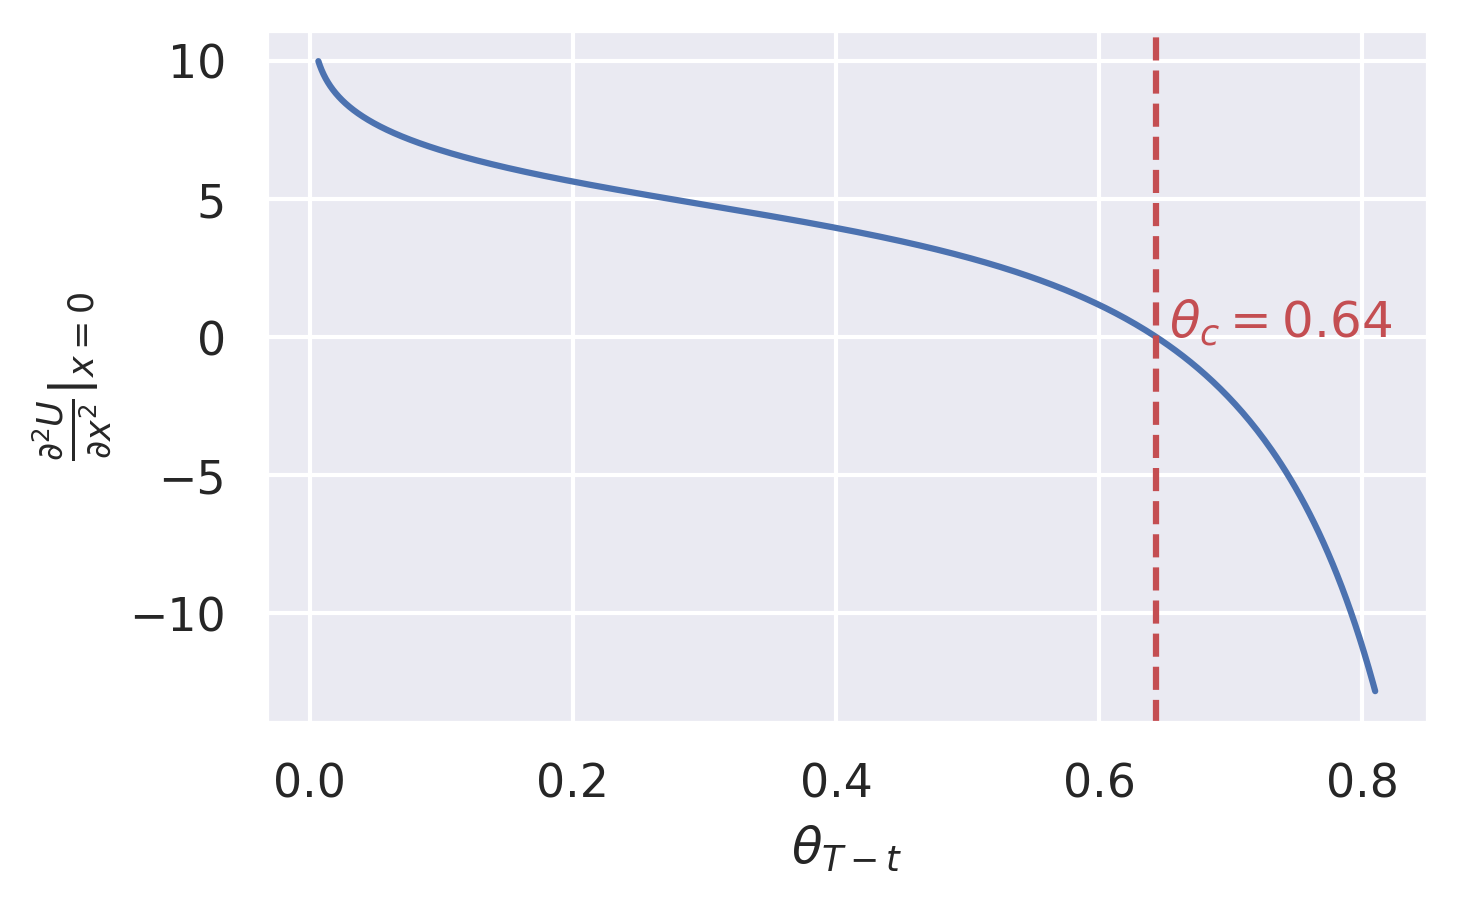
\includegraphics[width=0.4\textwidth]{figs/plots/critical_point_theta.png}
    \caption{Analysis of the stability of the fixed-point.}
    \label{fig:critical_point}
\end{figure}

\newpage
\subsubsection{All fixed-points}
We now provide the derivation to obtain all the fixed-points at a particular time by analysing its first derivative. For the sake of simplicity, we reorder the terms in the exponential inside the log term, resulting in the following expression:
\begin{align}
    u(x, t) &= -\beta(T - t) \left( \frac{1}{4} x^2 +  \log{\left(e^{\frac{(x - b)^2}{2 (b^2 -1)}} + e^{\frac{(x + b)^2}{2 (b^2 -1)}} \right)} \right)
\end{align}
Again for ease of notation we defined $b= \theta_{T-t}$, and note that we can derive from $\cosh(x) = \frac{e^x + e^{-x}}{2}$  the expression for $2\cosh(x) =  e^x + e^{-x}$, which we use to re-express the log term as follows:

\begin{align}
    \log{\left(e^{\frac{(x - b)^2}{2 (b^2 - 1)}} + e^{\frac{(x + b)^2}{2 (b^2-1)}} \right)} &=  \log{\left(e^{\frac{x^2 - 2xb+ b^2}{2 (b^2 - 1)}} + e^{\frac{x^2 + 2xb+b^2}{2 (b^2-1)}} \right)}\nonumber\\
    &=  \log{\left(e^{\frac{x^2 + b^2}{2 (b^2 - 1)}} \cdot e^{\frac{- xb}{b^2 - 1}}+ e^{\frac{x^2 +b^2}{2 (b^2-1)}} \cdot e^{\frac{xb}{b^2-1}}\right)}\nonumber\\
    &=  \log{\left(e^{\frac{x^2 + b^2}{2 (b^2 - 1)}} \cdot \left(e^{\frac{- xb}{b^2 - 1}}+  e^{\frac{xb}{b^2-1}}\right)\right)}\nonumber\\
    &=  \log{\left(e^{\frac{x^2 + b^2}{2 (b^2 - 1)}} \cdot 2\cosh(\frac{xb}{b^2-1}) \right)}\nonumber\\
    &=  \frac{x^2 + b^2}{2 (b^2 - 1)} + \log(2) + \log\left(\cosh(\frac{xb}{b^2-1}) \right)
\end{align}
Re-expressing the potential, we have:
\begin{equation}
    u(x, t) = -\beta(T - t) \left( \frac{1}{4} x^2 +   \frac{x^2 + b^2}{2 (b^2 - 1)} + \log\left(2\cosh(\frac{xb}{b^2-1}) \right) \right) + const
\end{equation}
computing its derivative we obtain the following
\begin{equation}
    \frac{d}{dx}u(x, t) =  -\beta(T- t) \left( \frac{1}{2} x +  \frac{x}{(b^2 - 1)} + \frac{b\tanh(\frac{xb}{b^2-1})}{(b^2 - 1)} \right)
\end{equation}
 Now we solve this equation for $\frac{d}{dx}u(x, t)=0$
 \begin{align}
 \frac{d}{dx}u(x, t) &= 0 = -\beta(T- t) \left( \frac{1}{2} x +  \frac{x}{(b^2 - 1)} + \frac{b\tanh(\frac{xb}{b^2-1})}{(b^2 - 1)} \right) \nonumber\\
    -\frac{1}{2} x -\frac{x}{(b^2 - 1)} &= \frac{b\tanh(\frac{xb}{b^2-1})}{(b^2 - 1)} \nonumber\\
        \frac{-x(b^2 - 1) - 2x}{2(b^2 - 1)} &= \frac{b\tanh(\frac{xb}{b^2-1})}{(b^2 - 1)} \nonumber\\
         \frac{-xb^2 +x - 2x}{2(b^2 - 1)} &= \frac{b\tanh(\frac{xb}{b^2-1})}{(b^2 - 1)} \nonumber\\
      \frac{-xb^2 - x}{2(b^2 - 1)} &= \frac{b\tanh(\frac{xb}{b^2-1})}{(b^2 - 1)} \nonumber\\
    -\frac{x(b^2 + 1)}{2(b^2 - 1)} &= \frac{b\tanh(\frac{xb}{b^2-1})}{(b^2 - 1)} \nonumber\\
     (b^2 + 1)x^{*} &= -2b\tanh(\frac{x^{*}b}{b^2-1})
 \end{align}




\subsection{Symmetry breaking in hyper-spherical diffusion models}
\label{supp:hyperspherical}

We will now analyze a more complex multivariate example where the data is sampled from the surface of a $D$-dimensional hyper-sphere. It is easy to see that in this case $G = O(D)$, since both the data distribution and the forward noise are spherically symmetric. Note that, while this is a highly simplified model, it does capture some properties of real data, since the Euclidean norm concentrates in high dimension. In this case, again up to constant terms, the potential is given by:
\begin{equation}
    u(\vect{x}, t) = -\beta(T - t) \left(\frac{1}{4} \norm{\vect{x}}{2}^2 + \log{\left(\int_{R^D} k(\vect{x}, T-t; \vect{x}', 0) \phi_D(\vect{x}'; r) \text{d} \vect{x}' \right)} \right)
\end{equation}

where $\phi_D(x'; r)$ is a Dirac `density' spherically symmetric and vanishing outside the surface of the hyper-sphere centered at the origin with radios equal to $r$. Unfortunately, the integral in the potential cannot be solved in closed form. However, it is possible to evaluate its Laplacian (i.e. the trace of the Hessian) at the origin, since the resulting integral only depends on the radial variable. In fact, the Laplacian of our potential at the origin is
\begin{equation}
% \label{eq:hyper-spherical laplacian}
     \nabla^2 u|_{x=0} = -\beta(T - t) \left(\frac{D}{2} +  \frac{(D + r^2) \theta_{T-t}^2 - D}{( \theta_{T-t}^2 - 1)^2} \right)
\end{equation}
In general, the sign of the Laplacian does not contain enough information to determine the stability of the fixed-point. However, in this case the Hessian matrix is a multiple of the identity matrix since all cross-derivatives vanish and all second derivatives have the same value. Consequently, we can determine the critical value of $\theta_{T-t}$ by checking when the Laplacian (and consequently all second derivatives), flips sign. The resulting equation gives us the critical value
\begin{equation}
    \theta_c = \sqrt{\frac{\sqrt{D^2 + r^2} - r}{D}}
\end{equation}
which reduces to Eq.~\ref{eq: critical theta 1d} for $r = 1$ and $D = 1$. The qualitative behavior of the hyper-spherical model is analogous to the one-dimensional model. When $\theta_{T-t} < \theta_c$, the origin is the only stable fixed-point. On the other hand, when $\theta_{T-t}$ becomes smaller than $\theta_c$, the origin becomes unstable while it appears a $D - 1$-dimensional manifolds of stable points consisting of the surface of a $D$-dimensional sphere centered at the origin with radius equal to  $\theta_{T-t} r$. Again, while the potential is spherically symmetric for all values of $\tau$, the symmetry is `broken' if we consider small perturbations of a single path, since the final position is in an arbitrary location on the surface of the sphere.



\subsection{Symmetry breaking in normalized datasets}
\label{supp:normalized_datasets_calculation}


\subsubsection{Fixed-points}
To derive the fixed-points of a diffusion model with $N$ i.i.d. data-points ${\vect{y}_1, \dots, \vect{y}_N} \in \mathbb{R}^D$, where the potential is described by Eq.~\ref{eq:potential_normalized_data}, we need to estimate the gradient of the potential function:


To compute the gradient of the potential, first we derive the gradient of the log term:
\begin{align}
    \frac{\partial}{\partial \vect{x}}(\log f(\vect{x})) &= \frac{1}{f(\vect{x})}\frac{\partial}{\partial \vect{x}}f(\vect{x}) \quad \quad  \text{with } f(\vect{x})=\sum_j e^{-\frac{\norm{\vect{x} - \theta_{T - t}\mathbf{y}_j}{2}^2}{2 ( 1 - \theta_{T-t}^2)}}\nonumber\\
    &= \frac{1}{f(\vect{x})}
    \sum_j e^{-\frac{\norm{\vect{x} - \theta_{T - t}\mathbf{y}_j}{2}^2}{2 ( 1 - \theta_{T-t}^2)}} \frac{\partial}{\partial \vect{x}}\left( -\frac{\norm{\vect{x} -  \theta_{T - t}\mathbf{y}_j}{2}^2}{2 ( 1 - \theta_{T-t}^2)}\right)\quad \quad \text{(chain rule)}\nonumber\\
    &= \frac{1}{f(\vect{x})}\left(-\sum_j e^{-\frac{\norm{\vect{x} -  \theta_{T - t}\mathbf{y}_j}{2}^2}{2 ( 1 - \theta_{T-t}^2)}} \frac{\vect{x} -  \theta_{T - t}\mathbf{y}_j}{ 1 - \theta_{T-t}^2}\right) \nonumber\\
    &= -\frac{1}{\sum_j e^{-\frac{\norm{\vect{x} - \theta_{T - t}\mathbf{y}_j}{2}^2}{2 ( 1 - \theta_{T-t}^2)}}}\sum_j e^{-\frac{\norm{\vect{x} -  \theta_{T - t}\mathbf{y}_j}{2}^2}{2 ( 1 - \theta_{T-t}^2)}} \frac{\vect{x} -  \theta_{T - t}\mathbf{y}_j}{ 1 - \theta_{T-t}^2}
\end{align}

For ease of notation, we express $b_j=  e^{-\frac{\norm{\vect{x} -  \theta_{T - t}\mathbf{y}_j}{2}^2}{2 ( 1 - \theta_{T-t}^2)}}$, and compute the gradient of the potential:
\begin{align}
   \frac{\partial}{\partial\vect{x}}u(\vect{x}, t)   &=   \frac{\partial}{\partial \vect{x}} \left( - \beta(T-t)
 \left(\frac{1}{4} ( \norm{\vect{x}}{2}^2 ) +    \log{\sum_j b_j } \right)\right) \nonumber\\
 &= - \beta(T - t) \left( \frac{1}{4}  \frac{\partial}{\partial \vect{x}}( \norm{\vect{x}}{2}^2 ) +    \frac{\partial}{\partial \vect{x}} \log{\sum_j b_j } \right) \nonumber\\
 &= - \beta(T - t) \left( \frac{1}{2}  \vect{x}   -\frac{1}{\sum_j b_j}\sum_j b_j \frac{\vect{x} -  \theta_{T - t}\mathbf{y}_j}{ 1 - \theta_{T-t}^2} \right)
\end{align}

solve the equation for $ \frac{\partial}{\partial\vect{x}}u(\vect{x}, t)   = 0$

\begin{align}
  \frac{\partial}{\partial\vect{x}}u(\vect{x}, t)   &= 0 = \beta(T - t) \left( -\frac{1}{2}  \vect{x} +  \frac{1}{\sum_j b_j}\sum_j b_j \frac{\vect{x} -  \theta_{T - t}\mathbf{y}_j}{ 1 - \theta_{T-t}^2} \right)  \nonumber\\
  \frac{1}{2}\vect{x} &= \frac{1}{\sum_j b_j}\sum_j (b_j \frac{\vect{x} - \theta_{T-t}\mathbf{y}_j}{ 1 - \theta_{T-t}^2}) \nonumber\\
   \frac{1}{2}\vect{x} &= \frac{1}{\sum_j b_j}\left(\sum_j  \frac{\vect{x}}{ 1 - \theta_{T-t}^2}b_j - \sum_j\frac{\theta_{T-t}\vect{y}_j}{ 1 - \theta_{T-t}^2}b_j\right) \nonumber\\
   \frac{1}{2}\vect{x} &= \frac{\vect{x}}{ 1 - \theta_{T-t}^2}\frac{\sum_j b_j }{\sum_j b_j} - \frac{\theta_{T-t}}{ 1 - \theta_{T-t}^2}\frac{1}{\sum_j b_j}\sum_j b_j \vect{y}_j  \nonumber\\
    \frac{1}{2}\vect{x} - \frac{\vect{x}}{ 1 - \theta_{T-t}^2} &= - \frac{\theta_{T-t}}{ 1 - \theta_{T-t}^2}\frac{1}{\sum_j b_j}\sum_j b_j \vect{y}_j \nonumber\\
     \frac{x(1 - \theta_{T-t}^2)-2\vect{x}}{ 2(1 - \theta_{T-t}^2)} &= - \frac{\theta_{T-t}}{ 1 - \theta_{T-t}^2}\frac{1}{\sum_j b_j}\sum_j b_j \vect{y}_j \nonumber\\
     -\vect{x}\frac{1 + \theta_{T-t}^2}{ 2(1 - \theta_{T-t}^2)} &= - \frac{\theta_{T-t}}{ 1 - \theta_{T-t}^2}\frac{1}{\sum_j b_j}\sum_j b_j \vect{y}_j  \nonumber\\
     \vect{x}\frac{1 + \theta_{T-t}^2}{ 2 \theta_{T-t}} &=   \frac{1}{\sum_j b_j}\sum_j b_j \vect{y}_j
\end{align}

Resulting in equation
\begin{equation}
    \frac{1+\theta_{T-t}^2}{2\theta_{T-t}} \vect{x} ^*= \frac{1}{\sum_j e^{w_j(\vect{x}^*; \theta_{T - t}) }}\sum_j e^{w_j(\vect{x}^*; \theta_{T - t}) } \vect{y}_j
\end{equation}


\newpage
\subsubsection{Critical point}

We assume data-points to be centered around zero, thus $\sum_j \vect{y}_j = 0~$, and perturbed samples $\vect{x}= \{x_1, \dots, x_D\} \in \mathbb{R}^D$. We denote a single coordinate point $x_i$ at coordinate $i$, then $\sum_i^D 1=D$.


The Laplacian of the potential function will be calculated as detailed below. A comprehensive derivation of the logarithmic term will subsequently follow:
\begin{align}
    \nabla^2 u(\vect{x}, t)&= \sum_i \frac{\partial^2}{\partial\vect{x}^2_i}u(\vect{x}, t)\nonumber\\
    &= \sum_i \frac{\partial^2}{\partial^2 x_i} \left( - \beta(T-t)
 \left(\frac{1}{4} ( \norm{\vect{x}}{2}^2 ) +    \log{\sum_j e^{-\frac{\norm{\vect{x} -  \theta_{T - t}\mathbf{y}_j}{2}^2}{2 ( 1 - \theta_{T-t}^2)}} } \right)\right) \nonumber\\
 &= - \beta(T - t) \left( \frac{1}{4} \sum_i \frac{\partial^2}{\partial^2 x_i}( \norm{\vect{x}}{2}^2 ) +   \sum_i \frac{\partial^2}{\partial^2 x_i} \log{\sum_j e^{-\frac{\norm{\vect{x} -  \theta_{T - t}\mathbf{y}_j}{2}^2}{2 ( 1 - \theta_{T-t}^2)}} } \right) \nonumber\\
 &=  - \beta(T - t)
 \left(\frac{D}{2} + \sum_i\frac{\partial^2}{\partial^2 x_i} \left( \log{\sum_j e^{-\frac{\norm{\vect{x} -  \theta_{T - t}\mathbf{y}_j}{2}^2}{2 ( 1 - \theta_{T-t}^2)}} } \right)\right) \nonumber\\
 &=  - \beta(T - t)
 \left(\frac{D}{2} + \sum_i\frac{\partial^2}{\partial^2 x_i} \left( \log{f(\vect{x}} )\right)\right) \nonumber\\
 &=  - \beta(T - t)
 \left(\frac{D}{2} + \sum_i \frac{-1}{1 - \theta_{T-t}^2}  +
        \frac{x_i^2}{(1 - \theta_{T-t}^2)^2}+
        \frac{\theta_{T - t}^2}{N(1 - \theta_{T-t}^2)^2}  \sum_j(\mathbf{y}_i^j)^2  \right) \nonumber\\
 &=  - \beta(T - t)
 \left(\frac{D}{2} +  \frac{-D}{1 - \theta_{T-t}^2}  +
        \frac{D x_i^2}{(1 - \theta_{T-t}^2)^2}+
        \frac{\theta_{T - t}^2}{N(1 - \theta_{T-t}^2)^2}  \sum_j\sum_i(y_i^j)^2  \right) \nonumber\\
 &=  - \beta(T - t)
 \left(\frac{D}{2} +  \frac{-D}{1 - \theta_{T-t}^2}  +
        \frac{D x_i^2}{(1 - \theta_{T-t}^2)^2}+
        \frac{\theta_{T - t}^2}{N(1 - \theta_{T-t}^2)^2}  \sum_j (\vect{y}_i^j)^2  \right) \nonumber\\
&=  - \beta(T - t)
 \left(\frac{D}{2} +  \frac{-D}{1 - \theta_{T-t}^2}  +
        \frac{D x_i^2}{(1 - \theta_{T-t}^2)^2}+
        \frac{\theta_{T - t}^2}{N(1 - \theta_{T-t}^2)^2}  \sum_j r^2  \right) \nonumber\\
\nabla^2 u(\vect{x}, t)|_{x=0} &=  - \beta(T - t) 
 \left(\frac{D}{2} +  \frac{-D}{1 - \theta_{T-t}^2} + \frac{\theta_{T - t}^2 r^2}{(1 - \theta_{T-t}^2)^2}\right) \nonumber\\
 &=  - \beta(T - t)
 \left(\frac{D}{2} +  \frac{-D(1 - \theta_{T-t}^2) + \theta_{T - t}^2 r^2}{(1 - \theta_{T-t}^2)^2}\right) \nonumber\\
  &=  - \beta(T - t)
 \left(\frac{D}{2} +  \frac{ (D  +  r^2)\theta_{T - t}^2 -D}{(1 - \theta_{T-t}^2)^2}\right) \nonumber\\
 &=  - \beta(T - t)
 \left(\frac{D}{2} +  \frac{ (D  +  r^2)\theta_{T - t}^2 -D}{(\theta_{T-t}^2 - 1)^2}\right) \nonumber\\
\end{align}



where $f(\vect{x})=\sum_j e^{-\frac{\norm{\vect{x} - \theta_{T - t}\mathbf{y}_j}{2}^2}{2 ( 1 - \theta_{T-t}^2)}}$. Utilizing the quotient rule, we estimated the second partial derivative of the logarithmic term as follows:

\begin{equation*}
    \frac{\partial^2}{\partial \vect{x}^2} (\log f(\vect{x})) = \frac{\partial}{\partial \vect{x}} \left( \frac{f^{'}(\vect{x})}{f(\vect{x})}  \right)= \frac{f^{''}(\vect{x})f(\vect{x}) - f^{'}(\vect{x})^2}{f(\vect{x})^2}\\
    =\frac{f^{''}(\vect{x})}{f(\vect{x})^2} \quad\quad \text{since } f^{'}(\vect{x})^2|_{x=0}=0
\end{equation*}

To compute the second partial derivative we do the following:

\begin{enumerate}
    \item First compute, we compute the first partial derivative of $f(\vect{x})$ by applying change rule again
    \begin{align}
        \frac{\partial}{\partial \vect{x}_i} f(\vect{x}) &= \sum_j \frac{\partial}{\partial x_i} e^{-\frac{\norm{\vect{x} - \theta_{T - t}\mathbf{y}_j}{2}^2}{2 ( 1 - \theta_{T-t}^2)}}\nonumber\\
        &=\sum_j  (-\frac{x_i - \theta_{T - t}\mathbf{y}_i^j}{1 - \theta_{T-t}^2}) e^{-\frac{\norm{\vect{x} - \theta_{T - t}\mathbf{y}_j}{2}^2}{2 ( 1 - \theta_{T-t}^2)}}\nonumber\\
        &=\sum_j \left(-\frac{1}{1 - \theta_{T-t}^2}  x_i   + \frac{\theta_{T - t}}{1 - \theta_{T-t}^2}\mathbf{y}_i^j \right) e^{-\frac{\norm{\vect{x} - \theta_{T - t}\mathbf{y}_j}{2}^2}{2 ( 1 - \theta_{T-t}^2)}}
    \end{align}
    \item Subsequently, the derivative of $ \frac{\partial}{\partial \vect{x}_i} f(\vect{x})$ is computed utilizing the product rule:
    \begin{align}
        &\frac{\partial^2}{\partial \vect{x}^2_i} f(\vect{x})\\ &=  \sum_j  \left(-\frac{1}{1 - \theta_{T-t}^2} e^{-\frac{\norm{\vect{x} - \theta_{T - t}\mathbf{y}_j}{2}^2}{2 ( 1 - \theta_{T-t}^2)}}  + (-\frac{x_i - \theta_{T - t}\mathbf{y}_i ^j}{1 - \theta_{T-t}^2})^2 e^{-\frac{\norm{\vect{x} - \theta_{T - t}\mathbf{y}_j}{2}^2}{2 ( 1 - \theta_{T-t}^2)}}\right) \nonumber\\
        &=  \sum_j  \left(-\frac{1}{1 - \theta_{T-t}^2}  + (-\frac{x_i - \theta_{T - t}\mathbf{y}_i^j}{1 - \theta_{T-t}^2})^2 \right) e^{-\frac{\norm{\vect{x} - \theta_{T - t}\mathbf{y}_j}{2}^2}{2 ( 1 - \theta_{T-t}^2)}} \nonumber\\
        &=  \sum_j  \left(-\frac{1}{1 - \theta_{T-t}^2}  +
        \frac{x_i^2}{(1 - \theta_{T-t}^2)^2}
        -\frac{2 x_i \theta_{T - t} y_i^j}{(1 - \theta_{T-t}^2)^2} +
        \frac{\theta_{T - t}^2 (y_i^j)^2}{(1 - \theta_{T-t}^2)^2} \right) e^{-\frac{\norm{\vect{x} - \theta_{T - t}\mathbf{y}_j}{2}^2}{2 ( 1 - \theta_{T-t}^2)}} \nonumber\\
        &=    \left(\frac{-N}{1 - \theta_{T-t}^2}  +
        \frac{N x_i^2}{(1 - \theta_{T-t}^2)^2}
        - \frac{2x_i \theta_{T - t}}{(1 - \theta_{T-t}^2)^2} \underbrace{\sum_j \mathbf{y}_i^j}_{= 0}+
        \frac{\theta_{T - t}^2}{(1 - \theta_{T-t}^2)^2} \sum_j(\mathbf{y}_i^j)^2 \right) e^{-\frac{\norm{\vect{x} - \theta_{T - t}\mathbf{y}_j}{2}^2}{2 ( 1 - \theta_{T-t}^2)}} \nonumber\\
       &=    \left(\frac{-N}{1 - \theta_{T-t}^2}  +
        \frac{N x_i^2}{(1 - \theta_{T-t}^2)^2}+
        \frac{\theta_{T - t}^2}{(1 - \theta_{T-t}^2)^2} N r^2 \right) e^{-\frac{\norm{\vect{x} - \theta_{T - t}\mathbf{y}_j}{2}^2}{2 ( 1 - \theta_{T-t}^2)}}
\end{align}
\item  We can now proceed to determine the second partial derivative:
   \begin{align}
        \frac{\partial^2}{\partial x_i^2} (\log f(\vect{x})) &=  \frac{f^{''}(\vect{x})}{f(\vect{x})} \nonumber\\
        &= \frac{  \left(\frac{-N}{1 - \theta_{T-t}^2}  +
        \frac{N x_i^2}{(1 - \theta_{T-t}^2)^2}+
        \frac{\theta_{T - t}^2}{(1 - \theta_{T-t}^2)^2}  \sum_j(\mathbf{y}_i^j)^2 \right) e^{-\frac{\norm{\vect{x} - \theta_{T - t}\mathbf{y}_j}{2}^2}{2 ( 1 - \theta_{T-t}^2)}} }{\sum_j e^{-\frac{\norm{\vect{x} - \theta_{T - t}\mathbf{y}_j}{2}^2}{2 ( 1 - \theta_{T-t}^2)}}}\nonumber\\
        &= \frac{  \left(\frac{-N}{1 - \theta_{T-t}^2}  +
        \frac{N x_i^2}{(1 - \theta_{T-t}^2)^2}+
        \frac{\theta_{T - t}^2}{(1 - \theta_{T-t}^2)^2}  \sum_j(\mathbf{y}_i^j)^2  \right) }{N}\nonumber\\
        &= \frac{-1}{1 - \theta_{T-t}^2}  +
        \frac{x_i^2}{(1 - \theta_{T-t}^2)^2}+
        \frac{\theta_{T - t}^2}{N(1 - \theta_{T-t}^2)^2}  \sum_j(\mathbf{y}_i^j)^2
   \end{align}
\end{enumerate}

\subsubsection{What happens at the origin?}

Here, we evaluate Eq.~\ref{eq: generalized self-consistency} at $\vect{x}^{*}=0$ to assess the behavior at the origin. The initial step involves evaluating the exponential term within the summation:
\begin{align}
    w_j(\vect{x}^*; \theta_{T - t})|_{\vect{x}^*=0} &= e^{-\norm{\vect{x}^* - \theta_{T - t} \vect{y}_j}{2}^2/(2(1 - \theta_{T - t}^2))}= e^{-\norm{\theta_{T - t} \vect{y}_j}{2}^2/(2(1 - \theta_{T - t}^2))} \nonumber\\
    &= e^{-\frac{\theta_{T - t}^2}{(2(1 - \theta_{T - t}^2))}\norm{ \vect{y}_j}{2}^2}\nonumber\\
    &= e^{-\frac{\theta_{T - t}^2}{(2(1 - \theta_{T - t}^2))}r^2}
\end{align}
Following this, we calculate the normalized weights at the origin for $N$ data points:
\begin{equation}
    \frac{w_j(\vect{0}; \theta_{T - t})}{\sum_j w_j(\vect{0}; \theta_{T - t})} = \frac{e^{-\frac{\theta_{T - t}^2}{(2(1 - \theta_{T - t}^2))}r^2}}{\sum_je^{-\frac{ \theta_{T - t}^2}{(2(1 - \theta_{T - t}^2))}r^2}} = \frac{1}{N}
\end{equation}

 Now, we  can evaluate Eq.~\ref{eq: generalized self-consistency}  at $\vect{x}^{*}=0$:
\begin{align}
    \frac{1 + \theta_{T - t}^2}{2 \theta_{T - t}} \vect{x}^* &= \frac{1}{\sum_j w_j(\vect{x}^*; \theta_{T - t})} \sum_j w_j(\vect{x}^*; \theta_{T - t}) \vect{y}_j \nonumber\\
    \vect{0}  &= \frac{1}{N} \sum_j \vect{y}_j \nonumber\\
    \vect{0}  &= \vect{0}
\end{align}

Under the two specific assumptions that 1) data points are centered around zero and 2) constrained to a fixed radius ($r^2 = \norm{ \vect{y}_j}{2}^2$), we have demonstrated that the origin indeed functions as a fixed point.

\section{Extended experiments}
\label{supp:experiments}




\subsection{Late start initialization}
\label{supp:late_start_init}

For completeness, Table~\ref{tab:ablation_fids} presents the resulting Fréchet Inception Distance (FID) scores, as illustrated in Figure \ref{fig:late_start_analysis}, for different late start times $s_{\text{start}} \ll T$. Table \ref{table:ablation_fids_mean} provides error bars computed from 4 runs. Figure~\ref{fig:main_image_2} visually demonstrates the unaffected performance of the CIFAR10 model during the early phase, even with fewer denoising steps. Notably, a late start at $s_{\text{start}} = 800$ yields better FID scores compared to $s_{\text{start}} = 1000$, resulting in a direct $20\%$ reduction in compute. Similarly, Figure \ref{fig:ls_visual_cifar10} illustrates generated samples for different late starts using the deterministic DDIM sampler, highlighting how a single starting point remains nearly unaffected in the early generative phase. Figure \ref{fig:ls_visual_celeba64}, \ref{fig:ls_visual_imagenet64}, \ref{fig:ls_visual_mnist} provide the same analysis but for Celeba64, Imagenet64 and MNIST respectively.









\begin{table}[ht!]
\centering
\resizebox{\textwidth}{!}{\begin{tabular}{c|ccccccccccc}
\toprule
\hline
\backslashbox{\textbf{Dataset}}{$s_{start}$} & 50 & 100 & 200 & 300 & 400 & 500 & 600 & 700& 800&900&1000\\
\hline
 MNIST    &  377.91& 295.00& 201.33& 55.47& 25.01& 14.14& 6.13& 2.12& 1.32& 1.21& 1.16\\\hline
 CIFAR10  & 381.77& 360.51& 283.74& 130.35& 23.47& 11.11& 5.02& 3.35& 3.11& 3.05& 3.18\\\hline
 CelebA   & 316.6& 318.04& 291.57& 148.23 & 39.85& 22.51& 9.76& 2.76&1.91 & 2.06& 2.15\\\hline
 Imagenet & 423.34& 443.77& 469.12& 456.90& 152.55& 45.24& 32.36& 26.5& 23.93& 22.89&  22.69\\\hline
 CelebA64 &424.13 &380.79 &371.05 &301.66 &81.16 &40.24 &23.11 &10.26 &3.39& 3.00& 3.27\\\hline
\midrule
\end{tabular}}
\caption{Analysis of image generation degradation measured in FID scores for different "late start" time $s_{start}$ for DDPM.}
\label{tab:ablation_fids}
\end{table}


\begin{table}[ht!]
\centering
\resizebox{\textwidth}{!}{\begin{tabular}{c|ccccccccccc}
\toprule
\hline
\backslashbox{\textbf{Dataset}}{$s_{start}$} & 50 & 100 & 200 & 300 & 400 & 500 & 600 & 700& 800&900&1000\\
\hline
MNIST    &  377.83 $\pm$ 0.15 & 295.07 $\pm$ 0.10 & 201.40 $\pm$ 0.27 & 55.64 $\pm$ 0.22 & 24.99 $\pm$ 0.03 & 13.99 $\pm$ 0.26 & 6.20 $\pm$ 0.05 & 2.12 $\pm$ 0.03 & 1.33 $\pm$ 0.01 & 1.22 $\pm$ 0.00 & 1.17 $\pm$ 0.01 \\\hline
CIFAR10  &  381.79 $\pm$ 0.04& 360.62 $\pm$ 0.07 & 283.90 $\pm$ 0.14 & 130.15 $\pm$ 0.17 & 23.69 $\pm$ 0.17 & 11.07 $\pm$ 0.05 & 4.98 $\pm$ 0.02 & 3.36 $\pm$ 0.02 & 3.06 $\pm$ 0.01 & 3.06 $\pm$ 0.03 & 3.08 $\pm$ 0.03 \\\hline
 CelebA   &  316.59 $\pm$ 0.05 & 318.11 $\pm$ 0.05 & 291.71 $\pm$ 0.09 & 148.40 $\pm$ 0.44 & 39.83 $\pm$ 0.04 & 22.50 $\pm$ 0.08 & 9.83 $\pm$ 0.06 & 2.82 $\pm$ 0.06 & 1.91 $\pm$ 0.01 & 2.08 $\pm$ 0.01 & 2.14 $\pm$ 0.02 \\\hline
 Imagenet & $423.42\pm 0.10$ & $443.79 \pm 0.04$ & 469.37  $\pm 0.30$ & 457.25 $\pm 0.37$ & 152.43 $\pm 0.47$  & 45.12 $\pm 0.10$  & 32.44 $\pm 0.05$  & 26.40 $\pm 0.09$ & 23.92 $\pm 0.07$  & $22.91 \pm 0.02$ & $22.68 \pm 0.03$ \\\hline
\midrule
\end{tabular}}
\caption{Mean FID scores and their associated standard deviations, obtained from a late-start initialization analysis across CIFAR10, MNIST, CelebA, and Imagenet, evaluated over 4 runs.}
\label{table:ablation_fids_mean}
\end{table}



\begin{figure}[ht!]
\minipage{0.216\textwidth}
  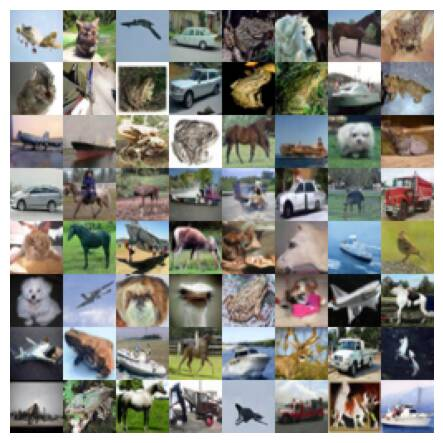
\includegraphics[width=\linewidth]{figs/imgs/ddpm_cifar10_data_samples_T_1000.jpg}
  \subcaption{\scriptsize  $T$=1000; FID=3.181} 
  \label{subfig:cifar10_1000}
\endminipage\hfill
\minipage{0.216\textwidth}
  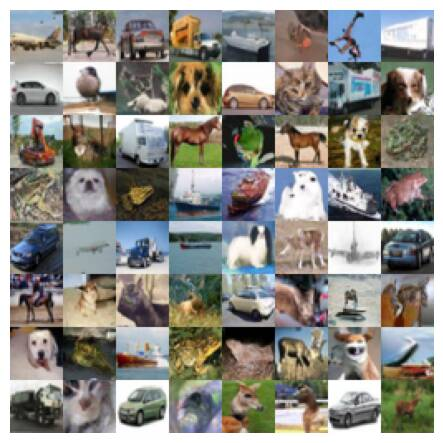
\includegraphics[width=\linewidth]{figs/imgs/ddpm_cifar10_data_samples_T_900.jpg}
  \subcaption{\scriptsize  $s_{start}$=900; FID=3.05} 
  \label{subfig:cifar10_900}
\endminipage\hfill
\minipage{0.216\textwidth}
  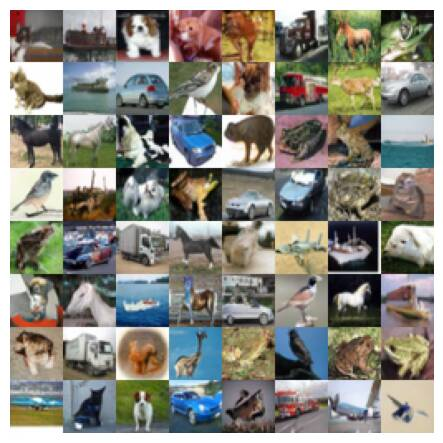
\includegraphics[width=\linewidth]{figs/imgs/ddpm_cifar10_data_samples_T_800.jpg}
  \subcaption{\scriptsize  $s_{start}$=800; FID=3.105}
  \label{subfig:cifar10_800}
\endminipage\hfill
\minipage{0.35\textwidth}
  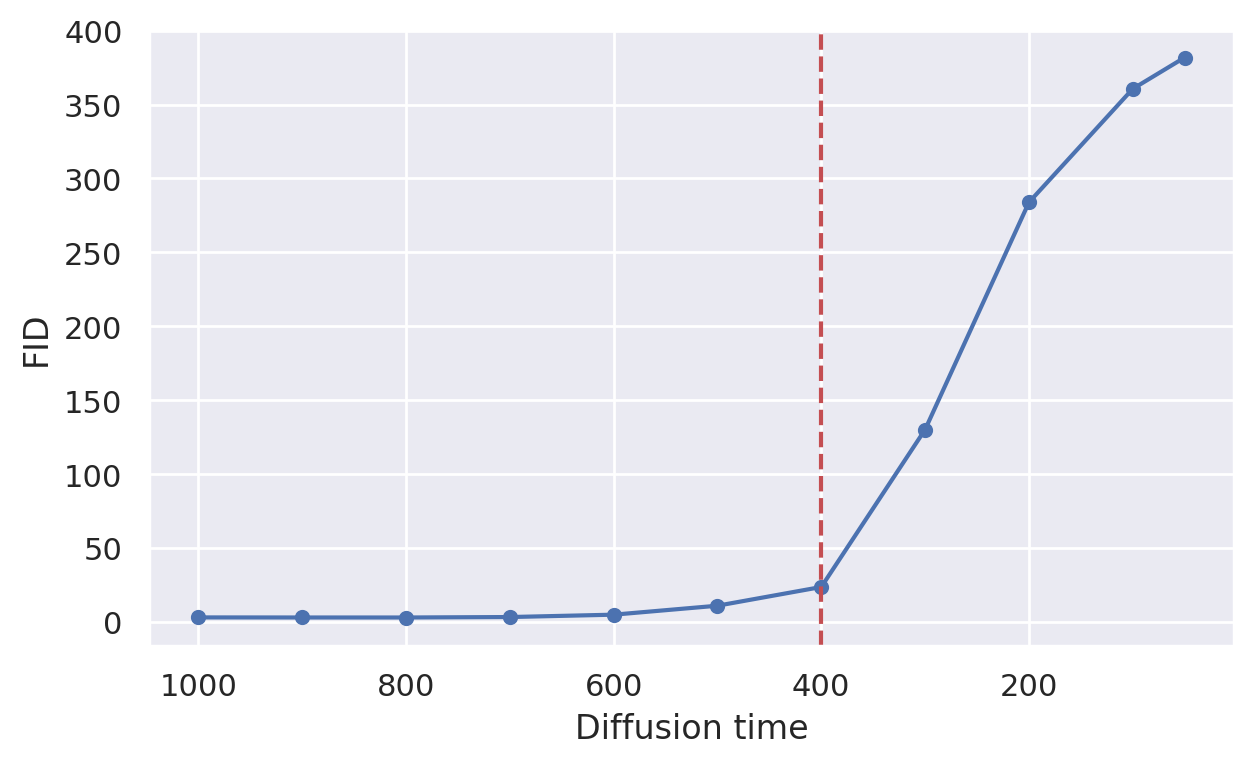
\includegraphics[width=\linewidth]{figs/plots/cifar10_late_start_fids_vl.png}
  \subcaption{Denoising start point $s_{start}$ vs FID} 
\endminipage\hfill
% second row
\minipage{0.216\textwidth}
  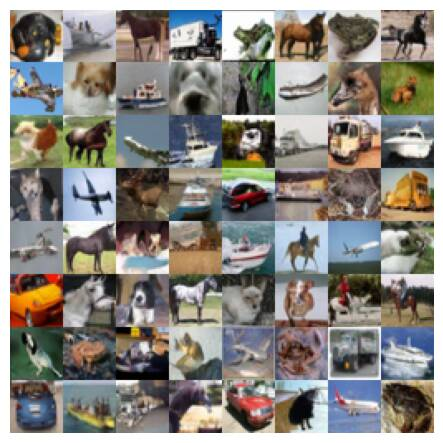
\includegraphics[width=\linewidth]{figs/imgs/ddpm_cifar10_data_samples_T_700.jpg}
  \subcaption{\scriptsize  $s_{start}$=700; FID=3.346}
\endminipage\hfill
\minipage{0.216\textwidth}
  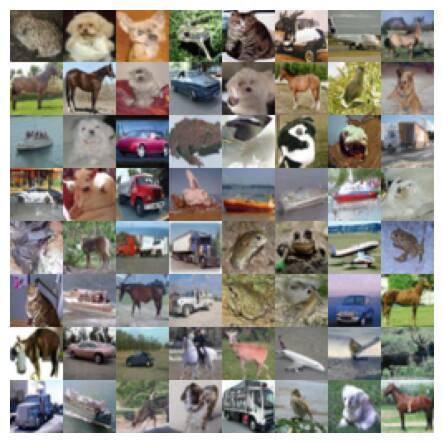
\includegraphics[width=\linewidth]{figs/imgs/ddpm_cifar10_data_samples_T_600.jpg}
  \subcaption{\scriptsize  $s_{start}$=600; FID=5.018}
\endminipage\hfill
\minipage{0.216\textwidth}
  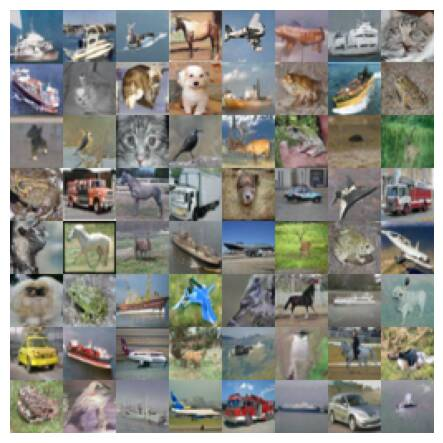
\includegraphics[width=\linewidth]{figs/imgs/ddpm_cifar10_data_samples_T_500.jpg}
  \subcaption{\scriptsize  $s_{start}$=500; FID=11.1}
\endminipage\hfill
\minipage{0.35\textwidth}
  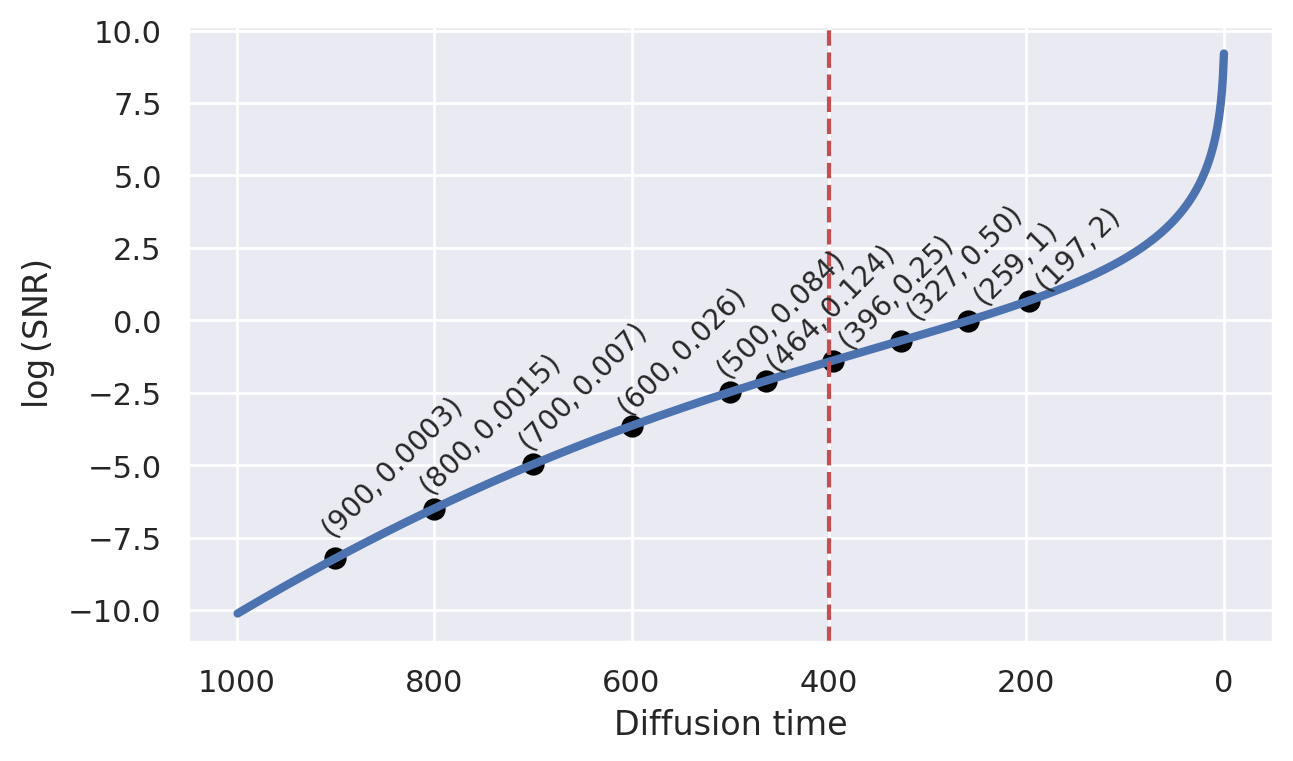
\includegraphics[width=\linewidth]{figs/plots/log_snr_analysis_vp_extended.png}
  \subcaption{SNR}
\endminipage\hfill
\minipage{0.355\textwidth}
    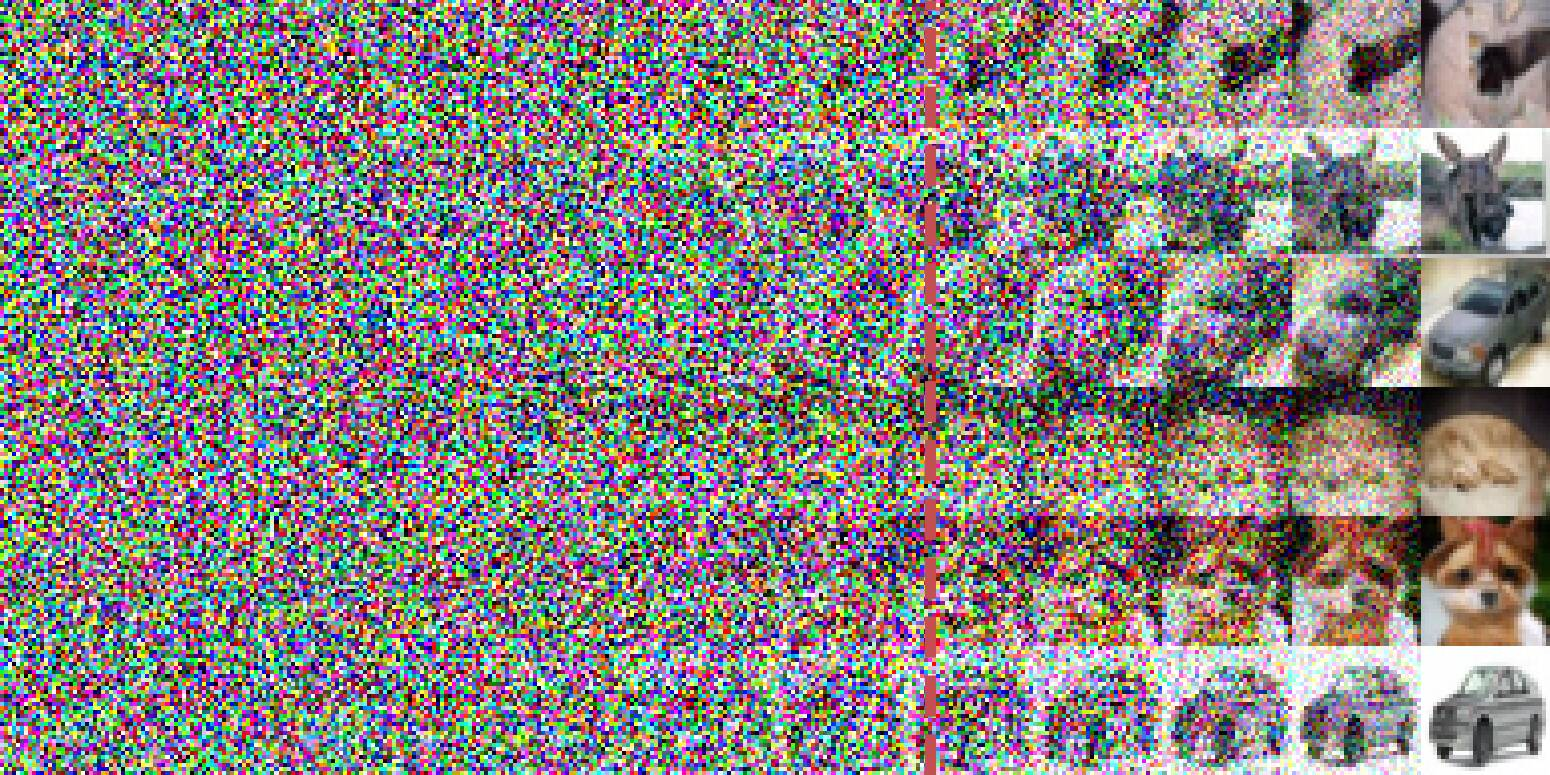
\includegraphics[width=\linewidth]{figs/imgs/cifar10_progressive_generation.jpg}
  \subcaption{Progressive generation}
\endminipage\hfill
\minipage{0.32\textwidth}
  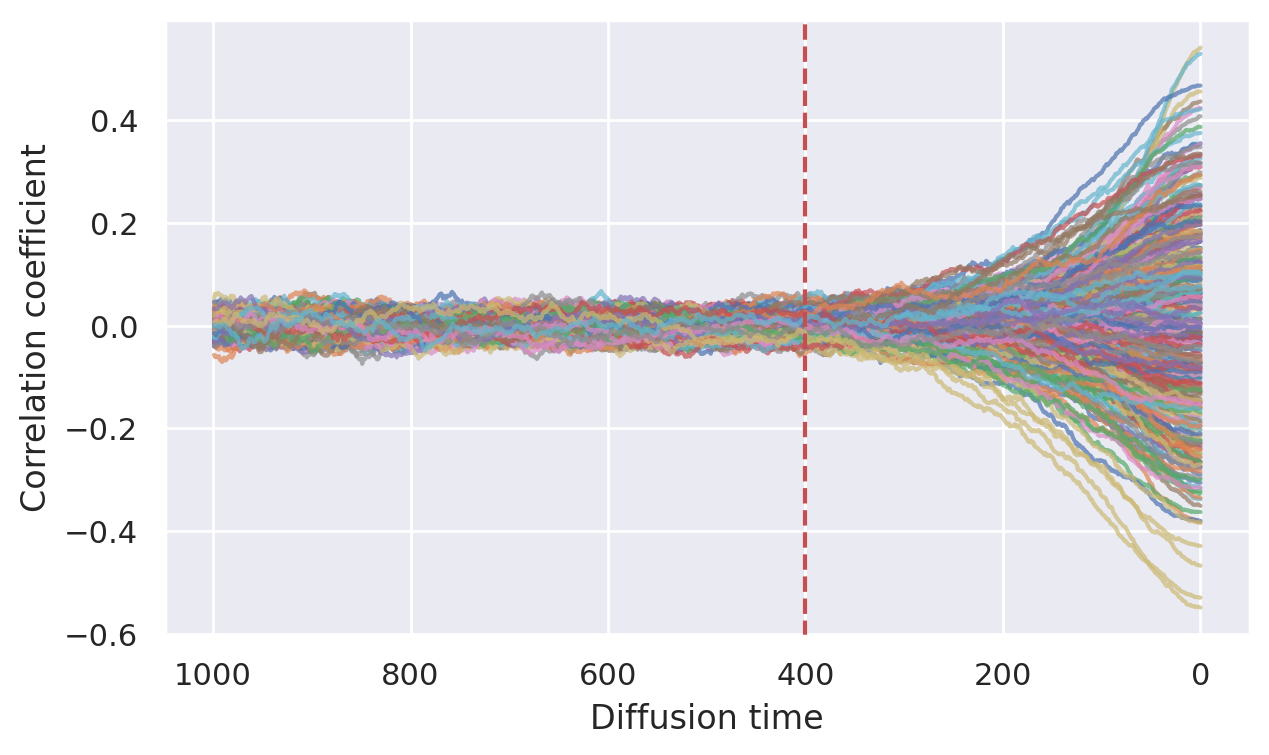
\includegraphics[width=\linewidth]{figs/plots/cifar10_correlation_trajectories.png}
  \subcaption{Correlation coefficient}
  % \label{subfig:correlation_coefficient}
\endminipage\hfill
\minipage{0.32\textwidth}
  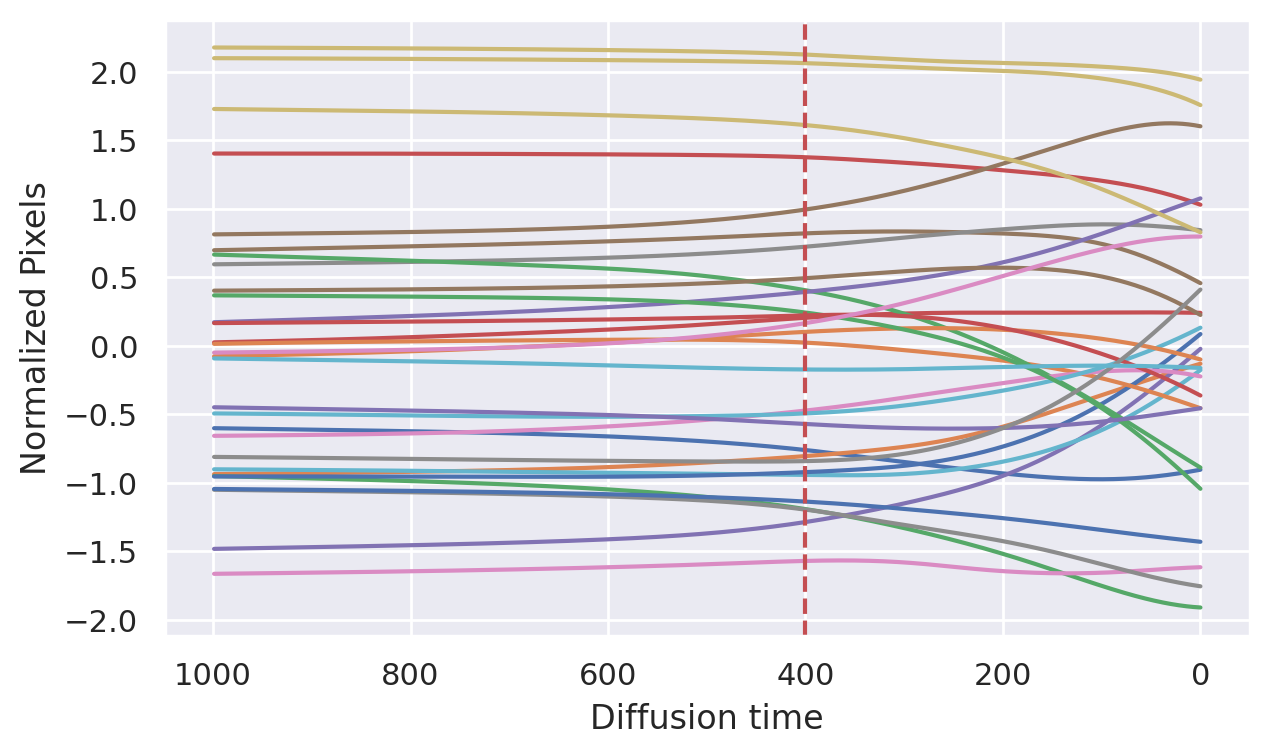
\includegraphics[width=\linewidth]{figs/plots/cifar10_normalized_trajectories.png}
  \subcaption{Normalized pixels}
   % \label{subfig:normalized_pixels}
\endminipage\hfill
\caption{Impact of starting the generative process at a late start $s_{start}=800 << T=1000$ on the model's performance. \textbf{a}) The standard generative process starting at $T=1000$. \textbf{b-g/d}) Depict the process when initiated at $s_{start}<<T=1000$. \textbf{d}) Resulting FID scores for different late start times $s_{\text{start}}<< T$. (i-k) Progressive generation and correlation and normalized pixel analysis (see Sec. \ref{sub:correlation_normalized}).}%
\label{fig:main_image_2}
\end{figure}


\begin{figure}[ht!]
\centering
\hspace*{-0.1in}%
\scalebox{0.48}{
      \begin{tikzpicture}[picture format/.style={inner sep=-0.25pt}]
      \node[picture format]                   (A1)             {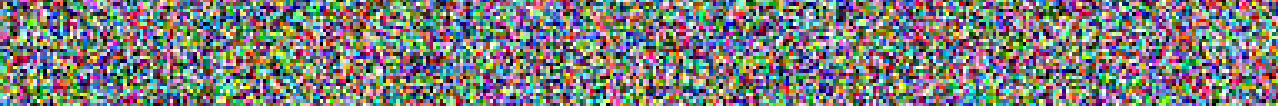
\includegraphics[width=0.92\textwidth]{figs/visuals/cifar10/ls_ddpm_ddim_cifar10_data_samples_T_100_12_hor.png}};
      \node[picture format,anchor=north]      (B1)   at (A1.south)           {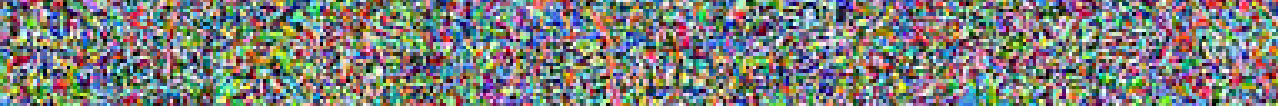
\includegraphics[width=0.92\textwidth]{figs/visuals/cifar10/ls_ddpm_ddim_cifar10_data_samples_T_200_12_hor.png}};
      \node[picture format,anchor=north]      (C1)   at (B1.south)           {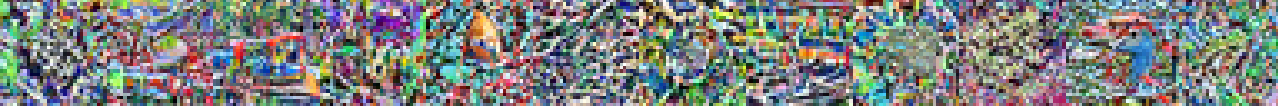
\includegraphics[width=0.92\textwidth]{figs/visuals/cifar10/ls_ddpm_ddim_cifar10_data_samples_T_300_12_hor.png}};
      \node[picture format,anchor=north]      (D1)   at (C1.south)           {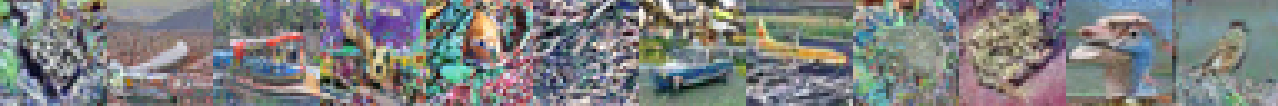
\includegraphics[width=0.92\textwidth]{figs/visuals/cifar10/ls_ddpm_ddim_cifar10_data_samples_T_400_12_hor.png}};
      \node[picture format,anchor=north]      (E1) at (D1.south) {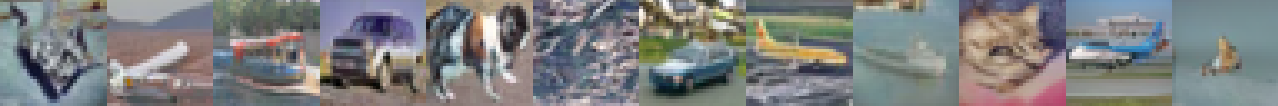
\includegraphics[width=0.92\textwidth]{figs/visuals/cifar10/ls_ddpm_ddim_cifar10_data_samples_T_500_12_hor.png}};
      \node[picture format,anchor=north]      (F1) at (E1.south) {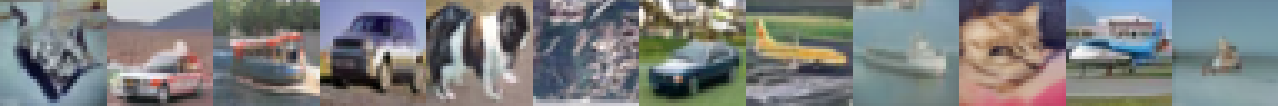
\includegraphics[width=0.92\textwidth]{figs/visuals/cifar10/ls_ddpm_ddim_cifar10_data_samples_T_600_12_hor.png}};
      \node[picture format,anchor=north]      (G1) at (F1.south) {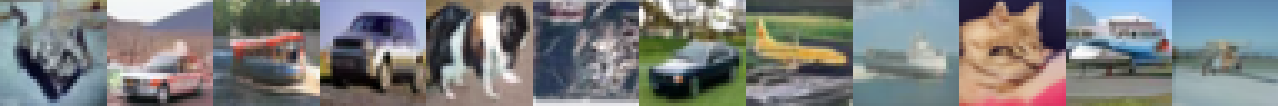
\includegraphics[width=0.92\textwidth]{figs/visuals/cifar10/ls_ddpm_ddim_cifar10_data_samples_T_700_12_hor.png}};
      \node[picture format,anchor=north]      (H1) at (G1.south) {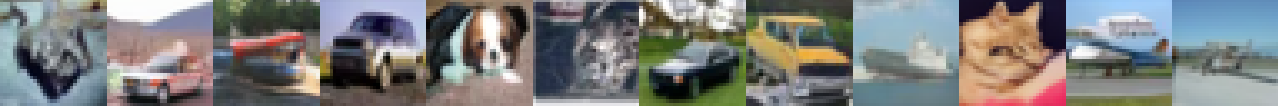
\includegraphics[width=0.92\textwidth]{figs/visuals/cifar10/ls_ddpm_ddim_cifar10_data_samples_T_800_12_hor.png}};
      \node[picture format,anchor=north]      (I1) at (H1.south) {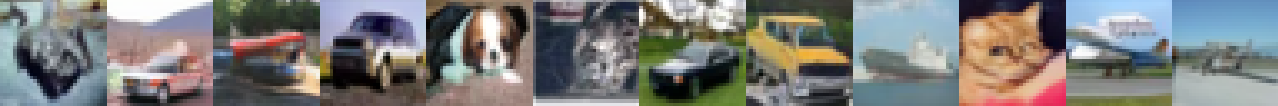
\includegraphics[width=0.92\textwidth]{figs/visuals/cifar10/ls_ddpm_ddim_cifar10_data_samples_T_900_12_hor.png}};
      \node[picture format,anchor=north]      (J1) at (I1.south) {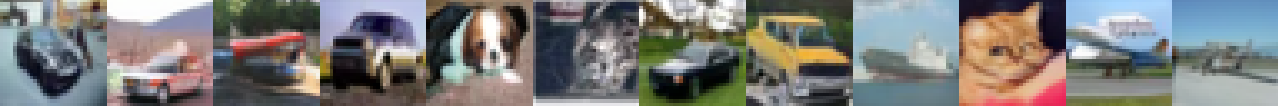
\includegraphics[width=0.92\textwidth]{figs/visuals/cifar10/ls_ddpm_ddim_cifar10_data_samples_T_999_12_hor.png}};
      %% Captions
      \node[anchor=east] (K1) at (A1.west) {\footnotesize\bfseries $s_{start}=100$};
      \node[anchor=east] (K2) at (B1.west) {\footnotesize\bfseries $s_{start}=200$};
      \node[anchor=east] (K3) at (C1.west) {\footnotesize\bfseries $s_{start}=300$};
      \node[anchor=east] (K4) at (D1.west) {\footnotesize\bfseries $s_{start}=400$};
      \node[anchor=east] (K5) at (E1.west) {\footnotesize\bfseries $s_{start}=500$};
      \node[anchor=east] (K6) at (F1.west) {\footnotesize\bfseries $s_{start}=600$};
      \node[anchor=east] (K7) at (G1.west) {\footnotesize\bfseries $s_{start}=700$};
      \node[anchor=east] (K8) at (H1.west) {\footnotesize\bfseries $s_{start}=800$};
      \node[anchor=east] (K9) at (I1.west) {\footnotesize\bfseries $s_{start}=900$};
      \node[anchor=east] (K10) at (J1.west) {\footnotesize\bfseries $T=1000$};
    \end{tikzpicture}
    }
\caption{Impact of a late initialization ($s_{\text{start}} \ll T=1000$) on CIFAR10 generation using the DDIM sampler, with starting times varied progressively from 1000 to 100. Despite the late start, the early phase remains largely unaffected since particles convergence to the fixed-point. The number of denoising steps matches each respective starting time, such as 1000 denoising steps for a start at 1000, and 100 for a start at 100.}
\label{fig:ls_visual_cifar10}
\end{figure}


\begin{figure}[ht!]
\centering
\scalebox{0.835}{
      \begin{tikzpicture}[picture format/.style={inner sep=-0.25pt}]
      \node[picture format]                   (A1)             {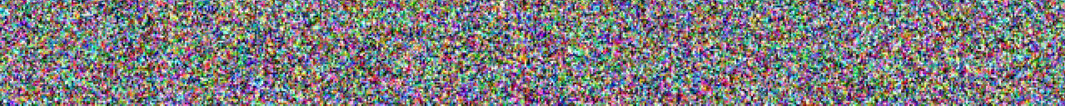
\includegraphics[width=0.85\textwidth]{figs/visuals/celeba64/ls_ddpm_ddim_celeba64_data_samples_T_100_10_hor.jpg}};
      \node[picture format,anchor=north]      (B1) at (A1.south) {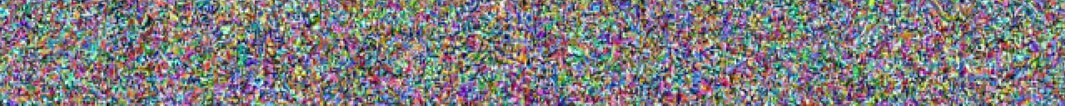
\includegraphics[width=0.85\textwidth]{figs/visuals/celeba64/ls_ddpm_ddim_celeba64_data_samples_T_200_10_hor.jpg}};
      \node[picture format,anchor=north]      (C1) at (B1.south) {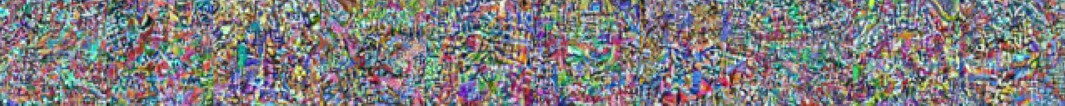
\includegraphics[width=0.85\textwidth]{figs/visuals/celeba64/ls_ddpm_ddim_celeba64_data_samples_T_300_10_hor.jpg}};
      \node[picture format,anchor=north]      (D1) at (C1.south) {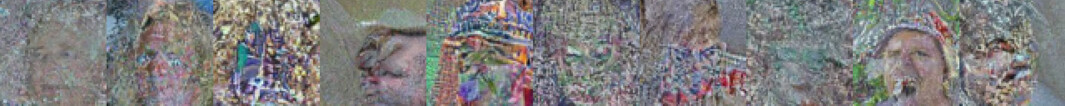
\includegraphics[width=0.85\textwidth]{figs/visuals/celeba64/ls_ddpm_ddim_celeba64_data_samples_T_400_10_hor.jpg}};
      \node[picture format,anchor=north]      (E1) at (D1.south) {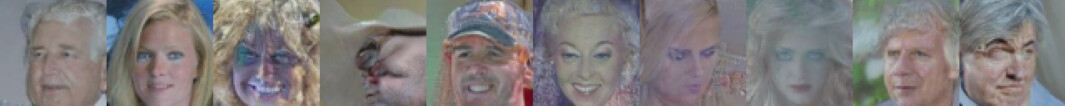
\includegraphics[width=0.85\textwidth]{figs/visuals/celeba64/ls_ddpm_ddim_celeba64_data_samples_T_500_10_hor.jpg}};
      \node[picture format,anchor=north]      (F1) at (E1.south) {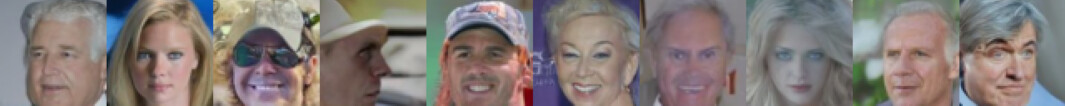
\includegraphics[width=0.85\textwidth]{figs/visuals/celeba64/ls_ddpm_ddim_celeba64_data_samples_T_600_10_hor.jpg}};
      \node[picture format,anchor=north]      (G1) at (F1.south) {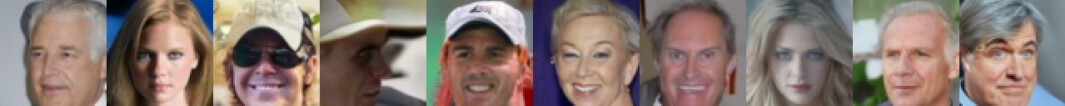
\includegraphics[width=0.85\textwidth]{figs/visuals/celeba64/ls_ddpm_ddim_celeba64_data_samples_T_700_10_hor.jpg}};
      \node[picture format,anchor=north]      (H1) at (G1.south) {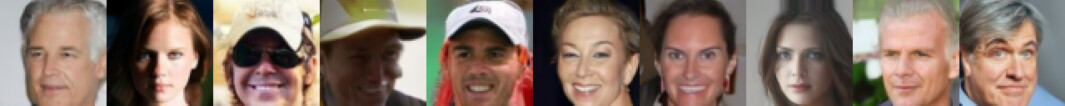
\includegraphics[width=0.85\textwidth]{figs/visuals/celeba64/ls_ddpm_ddim_celeba64_data_samples_T_800_10_hor.jpg}};
      \node[picture format,anchor=north]      (I1) at (H1.south) {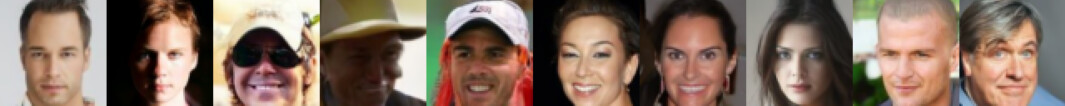
\includegraphics[width=0.85\textwidth]{figs/visuals/celeba64/ls_ddpm_ddim_celeba64_data_samples_T_900_10_hor.jpg}};
      \node[picture format,anchor=north]      (J1) at (I1.south) {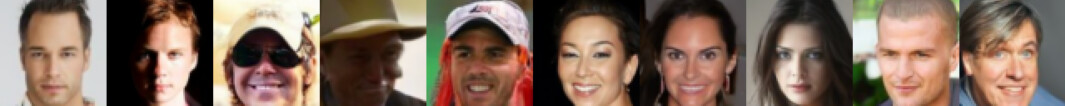
\includegraphics[width=0.85\textwidth]{figs/visuals/celeba64/ls_ddpm_ddim_celeba64_data_samples_T_999_10_hor.jpg}};
      %% Captions
      \node[anchor=east] (K1) at (A1.west) {\footnotesize\bfseries $s_{start}=100$};
      \node[anchor=east] (K2) at (B1.west) {\footnotesize\bfseries $s_{start}=200$};
      \node[anchor=east] (K3) at (C1.west) {\footnotesize\bfseries $s_{start}=300$};
      \node[anchor=east] (K4) at (D1.west) {\footnotesize\bfseries $s_{start}=400$};
      \node[anchor=east] (K5) at (E1.west) {\footnotesize\bfseries $s_{start}=500$};
      \node[anchor=east] (K6) at (F1.west) {\footnotesize\bfseries $s_{start}=600$};
      \node[anchor=east] (K7) at (G1.west) {\footnotesize\bfseries $s_{start}=700$};
      \node[anchor=east] (K8) at (H1.west) {\footnotesize\bfseries $s_{start}=800$};
      \node[anchor=east] (K9) at (I1.west) {\footnotesize\bfseries $s_{start}=900$};
      \node[anchor=east] (K10) at (J1.west) {\footnotesize\bfseries $T=1000$};
    \end{tikzpicture}
    }
\caption{Analogous impact of a late initialization ($s_{\text{start}} \ll T=1000$) on CelebA64 generation using the DDIM sampler, with starting times varied progressively from 1000 to 100. The denoising steps are set to match each respective starting time, demonstrating similar stability in the early phase.}
\label{fig:ls_visual_celeba64}
\end{figure}




\begin{figure}[ht!]
\centering
\scalebox{0.84}{
      \begin{tikzpicture}[picture format/.style={inner sep=-0.25pt}]
      \node[picture format]                   (A1)             {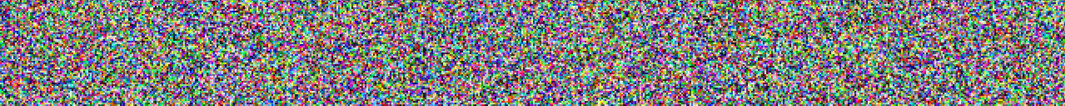
\includegraphics[width=0.85\textwidth]{figs/visuals/imagenet/ls_ddpm_ddim_imagenet64_data_samples_T_100_10_hor.jpg}};
      \node[picture format,anchor=north]      (B1) at (A1.south) {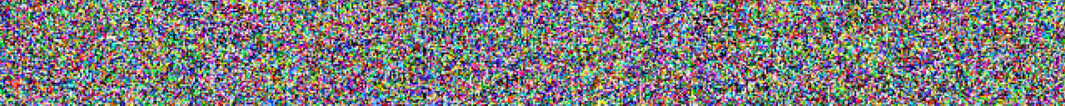
\includegraphics[width=0.85\textwidth]{figs/visuals/imagenet/ls_ddpm_ddim_imagenet64_data_samples_T_200_10_hor.jpg}};
      \node[picture format,anchor=north]      (C1) at (B1.south) {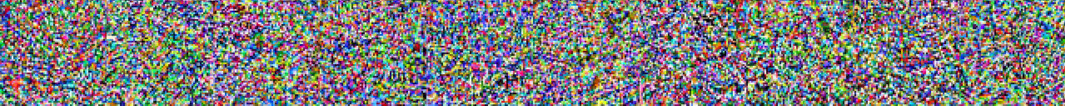
\includegraphics[width=0.85\textwidth]{figs/visuals/imagenet/ls_ddpm_ddim_imagenet64_data_samples_T_300_10_hor.jpg}};
      \node[picture format,anchor=north]      (D1) at (C1.south) {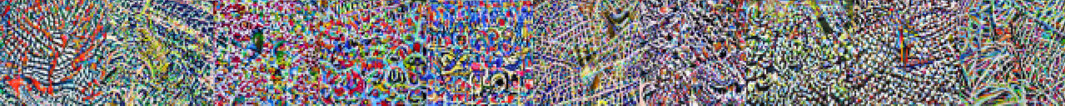
\includegraphics[width=0.85\textwidth]{figs/visuals/imagenet/ls_ddpm_ddim_imagenet64_data_samples_T_400_10_hor.jpg}};
      \node[picture format,anchor=north]      (E1) at (D1.south) {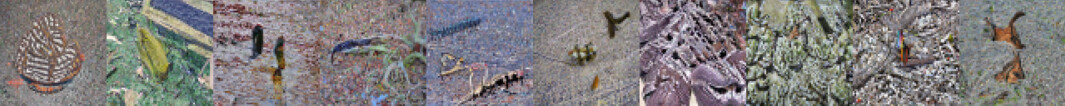
\includegraphics[width=0.85\textwidth]{figs/visuals/imagenet/ls_ddpm_ddim_imagenet64_data_samples_T_500_10_hor.jpg}};
      \node[picture format,anchor=north]      (F1) at (E1.south) {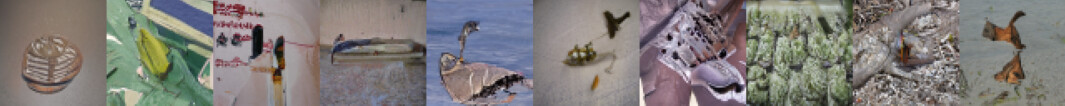
\includegraphics[width=0.85\textwidth]{figs/visuals/imagenet/ls_ddpm_ddim_imagenet64_data_samples_T_600_10_hor.jpg}};
      \node[picture format,anchor=north]      (G1) at (F1.south) {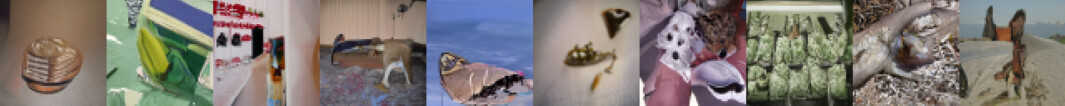
\includegraphics[width=0.85\textwidth]{figs/visuals/imagenet/ls_ddpm_ddim_imagenet64_data_samples_T_700_10_hor.jpg}};
      \node[picture format,anchor=north]      (H1) at (G1.south) {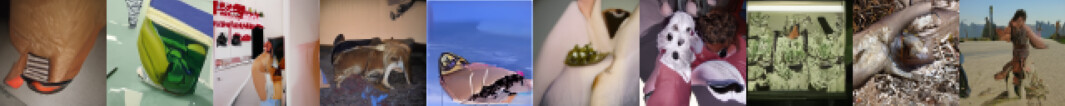
\includegraphics[width=0.85\textwidth]{figs/visuals/imagenet/ls_ddpm_ddim_imagenet64_data_samples_T_800_10_hor.jpg}};
      \node[picture format,anchor=north]      (I1) at (H1.south) {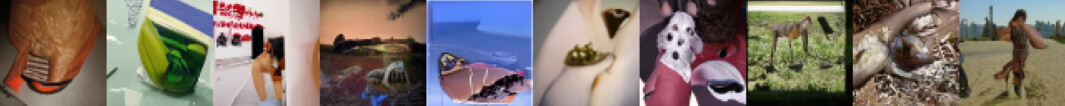
\includegraphics[width=0.85\textwidth]{figs/visuals/imagenet/ls_ddpm_ddim_imagenet64_data_samples_T_900_10_hor.jpg}};
      \node[picture format,anchor=north]      (J1) at (I1.south) {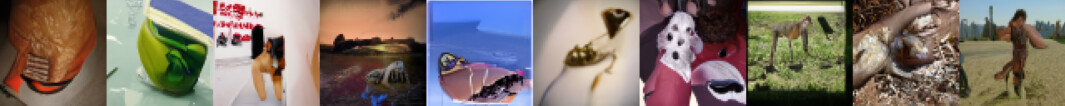
\includegraphics[width=0.85\textwidth]{figs/visuals/imagenet/ls_ddpm_ddim_imagenet64_data_samples_T_999_10_hor.jpg}};
      %% Captions
      \node[anchor=east] (K1) at (A1.west) {\footnotesize\bfseries $s_{start}=100$};
      \node[anchor=east] (K2) at (B1.west) {\footnotesize\bfseries $s_{start}=200$};
      \node[anchor=east] (K3) at (C1.west) {\footnotesize\bfseries $s_{start}=300$};
      \node[anchor=east] (K4) at (D1.west) {\footnotesize\bfseries $s_{start}=400$};
      \node[anchor=east] (K5) at (E1.west) {\footnotesize\bfseries $s_{start}=500$};
      \node[anchor=east] (K6) at (F1.west) {\footnotesize\bfseries $s_{start}=600$};
      \node[anchor=east] (K7) at (G1.west) {\footnotesize\bfseries $s_{start}=700$};
      \node[anchor=east] (K8) at (H1.west) {\footnotesize\bfseries $s_{start}=800$};
      \node[anchor=east] (K9) at (I1.west) {\footnotesize\bfseries $s_{start}=900$};
      \node[anchor=east] (K10) at (J1.west) {\footnotesize\bfseries $T=1000$};
    \end{tikzpicture}
    }
\caption{Analogous impact of a late initialization ($s_{\text{start}} \ll T=1000$) on Imagenet64 generation using the DDIM sampler, with starting times varied progressively from 1000 to 100. The denoising steps are set to match each respective starting time, demonstrating similar stability in the early phase.}
\label{fig:ls_visual_imagenet64}
\end{figure}



\clearpage
\begin{figure}[ht!]
\centering
\scalebox{0.7}{
      \begin{tikzpicture}[picture format/.style={inner sep=-0.25pt}]
      \node[picture format]                   (A1)             {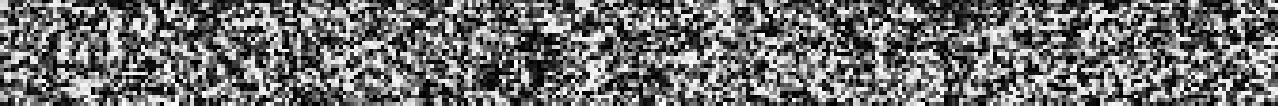
\includegraphics[width=0.85\textwidth]{figs/visuals/mnist/ls_ddpm_ddim_mnist_data_samples_T_100_12_hor.png}};
      \node[picture format,anchor=north]      (B1) at (A1.south) {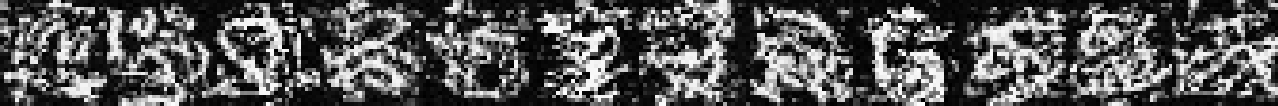
\includegraphics[width=0.85\textwidth]{figs/visuals/mnist/ls_ddpm_ddim_mnist_data_samples_T_200_12_hor.png}};
      \node[picture format,anchor=north]      (C1) at (B1.south) {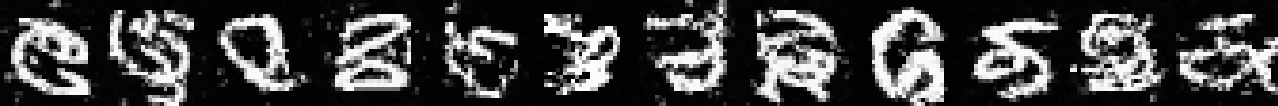
\includegraphics[width=0.85\textwidth]{figs/visuals/mnist/ls_ddpm_ddim_mnist_data_samples_T_300_12_hor.png}};
      \node[picture format,anchor=north]      (D1) at (C1.south) {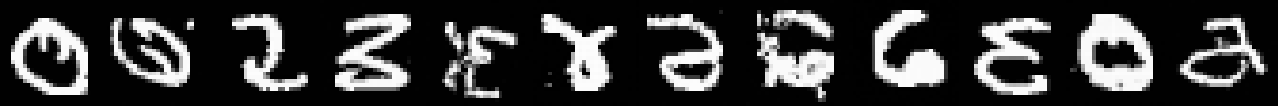
\includegraphics[width=0.85\textwidth]{figs/visuals/mnist/ls_ddpm_ddim_mnist_data_samples_T_400_12_hor.png}};
      \node[picture format,anchor=north]      (E1) at (D1.south) {\includegraphics[width=0.85\textwidth]{figs/visuals/mnist/ls_ddpm_ddim_mnist_data_samples_T_500_12_hor.png}};
      \node[picture format,anchor=north]      (F1) at (E1.south) {\includegraphics[width=0.85\textwidth]{figs/visuals/mnist/ls_ddpm_ddim_mnist_data_samples_T_600_12_hor.png}};
      \node[picture format,anchor=north]      (G1) at (F1.south) {\includegraphics[width=0.85\textwidth]{figs/visuals/mnist/ls_ddpm_ddim_mnist_data_samples_T_700_12_hor.png}};
      \node[picture format,anchor=north]      (H1) at (G1.south) {\includegraphics[width=0.85\textwidth]{figs/visuals/mnist/ls_ddpm_ddim_mnist_data_samples_T_800_12_hor.png}};
      \node[picture format,anchor=north]      (I1) at (H1.south) {\includegraphics[width=0.85\textwidth]{figs/visuals/mnist/ls_ddpm_ddim_mnist_data_samples_T_900_12_hor.png}};
      \node[picture format,anchor=north]      (J1) at (I1.south) {\includegraphics[width=0.85\textwidth]{figs/visuals/mnist/ls_ddpm_ddim_mnist_data_samples_T_999_12_hor.png}};
      %% Captions
      \node[anchor=east] (K1) at (A1.west) {\footnotesize\bfseries $s_{start}=100$};
      \node[anchor=east] (K2) at (B1.west) {\footnotesize\bfseries $s_{start}=200$};
      \node[anchor=east] (K3) at (C1.west) {\footnotesize\bfseries $s_{start}=300$};
      \node[anchor=east] (K1) at (D1.west) {\footnotesize\bfseries $s_{start}=400$};
      \node[anchor=east] (K2) at (E1.west) {\footnotesize\bfseries $s_{start}=500$};
      \node[anchor=east] (K3) at (F1.west) {\footnotesize\bfseries $s_{start}=600$};
      \node[anchor=east] (K4) at (G1.west) {\footnotesize\bfseries $s_{start}=700$};
      \node[anchor=east] (K5) at (H1.west) {\footnotesize\bfseries $s_{start}=800$};
      \node[anchor=east] (K6) at (I1.west) {\footnotesize\bfseries $s_{start}=900$};
      \node[anchor=east] (K7) at (J1.west) {\footnotesize\bfseries $T=1000$};
    \end{tikzpicture}
    }
\caption{Analogous impact of a late initialization ($s_{\text{start}} \ll T=1000$) on MNIST generation using the DDIM sampler, with starting times varied progressively from 1000 to 100. The denoising steps are set to match each respective starting time, demonstrating similar stability in the early phase.}
\label{fig:ls_visual_mnist}
\end{figure}


\subsection{Empirical analysis of the potential function in trained diffusion models}

\subsubsection{Method}
\label{sub:interpolation}
To visualize the potential for real high-dimensional datasets, we project the n-dimensional potential onto 1D by focusing only on the trajectory of two  sampled generative paths ($\vect{x}_1(t), \vect{x}_2$(t)) and representing the potential as a function of $\alpha$. In short, we do the following:
\begin{itemize}
    \item We run the sampler and obtain generative trajectory for $\vect{x}_1(t)$  and for $\vect{x}_2(t)$, obtaining $\vect{x}_{1T}, \dots, \vect{x}_{1t}, \vect{x}_{10}$  and   $\vect{x}_{2T}, \dots, \vect{x}_{2t}, \vect{x}_{20}$ corresponding sampled paths.
    \item We then obtained interpolated curves $\vect{x}(\alpha, t) = \cos(\alpha) \vect{x}_1(t) + \sin (\alpha) \vect{x}_2(t)$ (see Figure \ref{fig:interpolations}).
    \item We then compute the potential (up to a constant) as a function of $\alpha$ by
    $$\Tilde{u}(\alpha, t) = u(\vect{x}(\alpha), t)=\int_{-1}^{\alpha} \nabla U (\vect{x}(a), t) \cdot v da $$%
    in discrete time we estimate
    $$\Tilde{u}(\alpha_N, t) \approx \sum_{i=1}^N \nabla u (x(\alpha_i), t) \cdot v \Delta \alpha$$
    where $v= - \sin{\alpha} \vect{x}_1 +\cos{\alpha} \vect{x}_1  $
    \item Plot potential for $(\alpha, \Tilde{u}(\alpha, t))$ coordinates (see Section \ref{sub:plots_plotentials})
\end{itemize}

\begin{figure}[ht!]
\centering
\scalebox{0.9}{
      \begin{tikzpicture}[picture format/.style={inner sep=-0.25pt}]
      \node[picture format]                   (A1)             {\includegraphics[width=\textwidth]{figs/imgs/celeba64_interpolations_0_999.jpg}};
      \node[picture format,anchor=north]      (B1) at (A1.south) {\includegraphics[width=\textwidth]{figs/imgs/celeba64_interpolations_2_800.jpg}};
      \node[picture format,anchor=north]      (C1) at (B1.south) {\includegraphics[width=\textwidth]{figs/imgs/celeba64_interpolations_4_600.jpg}};
      \node[picture format,anchor=north]      (D1) at (C1.south) {\includegraphics[width=\textwidth]{figs/imgs/celeba64_interpolations_6_400.jpg}};
      \node[picture format,anchor=north]      (E1) at (D1.south) {\includegraphics[width=\textwidth]{figs/imgs/celeba64_interpolations_8_200.jpg}};
      \node[picture format,anchor=north]      (F1) at (E1.south) {\includegraphics[width=\textwidth]{figs/imgs/celeba64_interpolations_10_0.jpg}};
      %% Captions
      \node[anchor=east] (J1) at (A1.west) {\footnotesize\bfseries $0$};
      \node[anchor=east] (J2) at (B1.west) {\footnotesize\bfseries $200$};
      \node[anchor=east] (J3) at (C1.west) {\footnotesize\bfseries $400$};
      \node[anchor=east] (J4) at (D1.west) {\footnotesize\bfseries $600$};
      \node[anchor=east] (J5) at (E1.west) {\footnotesize\bfseries $800$};
      \node[anchor=east] (J6) at (F1.west) {\footnotesize\bfseries $1000$};
    \end{tikzpicture}
    }
\caption{VP interpolations of two sampled paths $\vect{x}_1(t)$ and $\vect{x}_2(t)$ over $\alpha \in [-\frac{1}{5}\pi , \frac{7}{10}\pi]$.}
\label{fig:interpolations}
\end{figure}



\clearpage
\subsubsection{Plots of potentials}
\label{sub:plots_plotentials}
This section presents 1D sections plots of the potential of diffusion models trained on CIFAR10, ImageNet64 and CelebA64, along with corresponding generated samples in Figures \ref{fig:potentials_cifar10}, \ref{fig:potentials_imagenet64}, and \ref{fig:potentials_celeba64}.

\begin{figure}[ht!]
\centering
\begin{minipage}[b]{.368\textwidth}
\subfloat
  []{\includegraphics[width=\textwidth]{figs/imgs/cifar10_samples.jpg}}
\end{minipage}%
\begin{minipage}[b]{.625\textwidth}
\centering
\stepcounter{subfigure} % Increment subfigure counter
\subfloat
  {\includegraphics[width=\textwidth]{figs/plots/potentials_cifar10_avg_20.png}}\vfill
\addtocounter{subfigure}{-2}
\subfloat[]
  {\includegraphics[width=\textwidth]{figs/imgs/cifar10_progressive_generation_2.jpg}}
\end{minipage}
\caption{Symmetry breaking in CIFAR10: (a) Generated samples; (b) Time-varied 1D potential sections (top figure) from a trained diffusion model along circular paths between two samples (bottom figure), averaged over 20 generated samples from (a).}
\label{fig:potentials_cifar10}
\end{figure}


\begin{figure}[ht!]
\centering
\begin{minipage}[b]{.368\textwidth}
\subfloat
  []{\includegraphics[width=\textwidth]{figs/imgs/imagenet64_samples.jpg}}
\end{minipage}%
\begin{minipage}[b]{.625\textwidth}
\centering
\stepcounter{subfigure} % Increment subfigure counter
\subfloat
  {\includegraphics[width=\textwidth]{figs/plots/potentials_imagenet64_avg_20.png}}\vfill
\addtocounter{subfigure}{-2}
\subfloat[]
  {\includegraphics[width=\textwidth]{figs/imgs/imagenet64_progressive_generation_2.png}}
\end{minipage}
\vspace{-0.1cm}
\caption{Symmetry breaking in Imagenet64.}
\label{fig:potentials_imagenet64}
\end{figure}

\begin{figure}[ht!]
\centering
\begin{minipage}[b]{.368\textwidth}
\subfloat
  []{\includegraphics[width=\textwidth]{figs/imgs/celeba64_samples.jpg}}
\end{minipage}%
\begin{minipage}[b]{.625\textwidth}
\centering
\stepcounter{subfigure} % Increment subfigure counter
\subfloat
  {\includegraphics[width=\textwidth]{figs/plots/potentials_celeba64_avg_20.png}}\vfill
\addtocounter{subfigure}{-2}
\subfloat[]
  {\includegraphics[width=\textwidth]{figs/imgs/celeba64_progressive_generation_2.png}}
\end{minipage}
\caption{Symmetry breaking in CelebA64.}
\vspace{-0.1cm}
\label{fig:potentials_celeba64}
\end{figure}

% \newpage
\clearpage
\subsection{Correlation coefficients and Normalized pixel trajectories}
\label{sub:correlation_normalized}

In order to qualitatively investigate the generative dynamics of diffusion models, we analyze correlation and normalized pixel trajectories along the generative paths. The correlation coefficient trajectories reveal the evolution of sample correlations over time, highlighting the transition from uncorrelated to aligned samples. By comparing a fixed/reference trajectory with multiple trajectories, we construct correlation trajectories. Furthermore, we track the changes in pixel values using normalized pixel trajectories. Initially, during the early generation phase, the pixel values remain unchanged without any discernible patterns or transformations. However, beyond a critical point, the normalized pixels show the emergence of features and patterns. Our analyses utilize a batch of 300 samples for correlation trajectories and over 500 generated samples for normalized trajectories. The normalized trajectories are sampled using the deterministic DDIM sampler, showcasing both stochastic and deterministic behavior.

\begin{figure}[ht!]
\centering
\minipage{0.35\textwidth}
    \includegraphics[width=\linewidth]{figs/imgs/mnist_progressive_generation.jpg}
  \subcaption{MNIST Progressive generation}
\endminipage\hfill
\minipage{0.32\textwidth}
  \includegraphics[width=\linewidth]{figs/plots/mnist_correlation_trajectories.png}
  \subcaption{Correlation coefficient}
\endminipage\hfill
\minipage{0.32\textwidth}
  \includegraphics[width=\linewidth]{figs/plots/mnist_normalized_trajectories.png}
  \subcaption{Normalized pixels}
\endminipage\hfill
\minipage{0.35\textwidth}
    \includegraphics[width=\linewidth]{figs/imgs/celeba_progressive_generation.png}
  \subcaption{CelebA32 Progressive generation}
\endminipage\hfill
\minipage{0.32\textwidth}
  \includegraphics[width=\linewidth]{figs/plots/celeba_correlation_trajectories.png}
  \subcaption{Correlation coefficient}
\endminipage\hfill
\minipage{0.32\textwidth}
  \includegraphics[width=\linewidth]{figs/plots/celeba_normalized_trajectories.png}
  \subcaption{Normalized pixels}
\endminipage\hfill

\minipage{0.35\textwidth}
    \includegraphics[width=\linewidth]{figs/imgs/imagenet64_progressive_generation.png}
  \subcaption{Imagenet64 Progressive generation}
\endminipage\hfill
\minipage{0.32\textwidth}
  \includegraphics[width=\linewidth]{figs/plots/imagenet64_correlation_trajectories.png}
  \subcaption{Correlation coefficient}
\endminipage\hfill
\minipage{0.32\textwidth}
  \includegraphics[width=\linewidth]{figs/plots/imagenet64_normalized_trajectories_flipped.png}
  \subcaption{Normalized pixels}
\endminipage\hfill


\minipage{0.35\textwidth}
    \includegraphics[width=\linewidth]{figs/imgs/celeba64_progressive_generation.png}
  \subcaption{CelebA64 Progressive generation}
\endminipage\hfill
\minipage{0.32\textwidth}
  \includegraphics[width=\linewidth]{figs/plots/celeba64_correlation_trajectories.png}
  \subcaption{Correlation coefficient}
\endminipage\hfill
\minipage{0.32\textwidth}
  \includegraphics[width=\linewidth]{figs/plots/celeba64_normalized_trajectories_flipped.png}
  \subcaption{Normalized pixels}
\endminipage\hfill
\caption{Progressive generation and trajectory analysis: Correlation and normalized pixel evolution in diffusion models over time.}%
\end{figure}



\newpage
\section{Fast Samplers}
\label{supp:fast_samplers_performance}



\subsection{Table results}
This section provides comprehensive empirical analysis on model performance for varied start times, comparing the Gaussian initialization with vanilla samplers. Table~\ref{tab:fast_sampling_late_start} details results for deterministic samplers like DDIM and PSNDM, while Table~\ref{tab:fast_sampling_late_start_ddpm} focuses on stochastic DDPM. These tables include FID scores and consider a fixed number of equally spaced denoising steps. Table~\ref{tab:extended_results} extends these results for higher numbers of functions evaluations (NFEs), confirming FID improvements at higher NFEs. Figure~\ref{fig:gaussianity-test} validates the Gaussianity assumption in the early generative phase.


\begin{table}[ht!]
\centering
\resizebox{\textwidth}{!}{\begin{tabular}{c|c|ccccccccccc}
\toprule
\hline
\textbf{Dataset} & \backslashbox{model}{$s_{start}$} & 50 & 100 & 200 & 300 & 400 & 500 & 600 & 700& 800&900&1000\\
\hline
        & DDIM-10   & 397.7 & 364.05 & 287.79 & 174.14& 42.65 & 18.06 & 10.01 & 5.81 & \textbf{4.40}& \textcolor{cyan!}{\textbf{4.46}}&5.03\\
        & DDIM-10\textsuperscript{\textdagger} &163.22 &163.83 &104.34 &28.98 &6.07 &\textbf{2.44} &2.5 &3.05 &3.57 &4.20 &4.80 \\
        & DDIM-05 & 397.75& 362.82& 283.78& 167.02& 43.65& 19.69& 13.08& \textbf{10.11}& \textcolor{cyan!}{\textbf{10.69}}& 12.92& 16.06\\
        & DDIM-05\textsuperscript{\textdagger} &162.92& 160.62& 96.96& 25.73& 7.28& \textbf{5.24}& 6.16& 7.80& 9.92& 12.47& 15.77 \\
        & DDIM-03 &397.49 &359.51 &271.84 &151.35  &50.50 &\textbf{29.5} &30.01 &37.93 &52.11 &73.81 &102.28 \\
MNIST  & DDIM-3\textsuperscript{\textdagger} &162.11 &155.72 &84.09 &22.73 &\textbf{11.50} &13.32 &20.97 &34.60 &50.96 &73.547 &102.70\\
        & PSDM-10 &398.45 &366.40 &290.22 & 188.32& 57.63 & 27.80 & 17.83&\textbf{12.40}&17.15&\textcolor{cyan!}{\textbf{14.36}}& 15.00\\
        & PSDM-10\textsuperscript{\textdagger} &165.47 &167.99 &113.20 &35.25 &9.35 &\textbf{5.02} &5.78 &7.31 &14.75 &13.32 &14.77 \\
        & PSDM-05 & 398.47& 367.91& 293.90& 183.42& 51.29& 23.49& 18.72& \textbf{18.01}& \textcolor{cyan!}{\textbf{21.22}}& 21.18& 21.34\\
        & PSDM-05\textsuperscript{\textdagger} &165.68 &168.53 &115.43 &33.77 &8.70 &\textbf{5.11} &7.28 &11.89 &18.68 &20.33 &21.54 \\
        & PSDM-03 &398.81 &367.92 &288.95 &207.45 &123.95 &\textbf{110.05} &119.18 &154.89 &220.26 &273.10 &381.89 \\
        & PSDM-3\textsuperscript{\textdagger} &165.23 &166.11 &117.72 &43.49 &\textbf{38.23} &64.41 &98.1 &148.49 &218.91 &271.59 &381.15\\
        \hline
        & DDIM-10 & 410.13 & 376.91 & 334.41 & 229.93& 57.18 & 17.98 & \textbf{15.65}& 16.57&18.39& \textcolor{cyan!}{\textbf{19.79}}&21.27\\
        & DDIM-10\textsuperscript{\textdagger} & 139.41& 89.97& 48.30& 28.66& 19.36& \textbf{15.98}& 16.14& 17.03& 18.50& 19.54& 21.12\\
        & DDIM-5 &409.17&375.47&330.77&210.12&51.78&\textbf{29.97}&33.55&38.28&\textcolor{cyan!}{\textbf{44.61}}&51.31&56.68\\
        & DDIM-5\textsuperscript{\textdagger}  & 132.58& 86.59& 49.85& 33.72& 26.88& \textbf{26.36}& 30.13& 36.29& 44.26& 51.46& 56.68\\ 
        & DDIM-03 &407.79 &373.01 &320.84 &190.75 &71.77 &\textbf{68.01} &85.93 &109.37 &133.53 &144.55 &129.76\\ 
 CIFAR10& DDIM-3\textsuperscript{\textdagger} &125.29 &84.14 &54.08 &42.84 &\textbf{42.31} &51.8 &72.86 &102.88 &131.68 &144.51 &128.91 \\
        & PSDM-10 & 412.60 & 379.25& 337.89 & 247.44 & 75.76& 17.36& 7.75& \textbf{6.20} & 7.31 & \textcolor{cyan!}{\textbf{8.35}} & 8.07\\
        & PSDM-10\textsuperscript{\textdagger} &150.39 &95.77 &45.97 &22.09 &10.81 &6.72 &\textbf{5.90} &6.24 &7.41 &8.23 &8.07 \\
        & PSDM-05 & 412.49& 379.41& 340.89& 236.68& 63.11& 17.78& \textbf{11.13}& 11.34& \textcolor{cyan!}{\textbf{13.77}}& 17.56& 26.15\\
        & PSDM-05\textsuperscript{\textdagger} &149.778 &92.62 &44.49 &21.97 &12.41 &\textbf{9.55} &10.17 &11.79 &13.94 &17.72 &25.73 \\
        & PSDM-03 &412.76 &379.27 &339.22 &252.22 &134.77 &80.94 &\textbf{78.20} &103.11 &170.68 &266.32 &407.46 \\ 
        & PSDM-3\textsuperscript{\textdagger} &149.63 & 96.97&53.34 &37.10 &\textbf{34.20} &44.98 &65.78 &99.46 &169.76 &265.58 &407.63\\
        \hline
        & DDIM-10 & 345.98 & 316.55 & 306.08 & 251.90& 68.03 & 25.67 & 25.67& 15.86&\textbf{10.83}& \textcolor{cyan!}{\textbf{11.37}}&13.94\\
        & DDIM-10\textsuperscript{\textdagger} &65.45 &34.5 &12.80 &7.89 &\textbf{7.27} &8.57 &10.00 &11.81 &13.38 &15.32 &16.81 \\
        & DDIM-05 & 344.04& 316.53& 303.82& 237.93& 55.65& 28.74& 22.11& \textbf{20.03}& \textcolor{cyan!}{\textbf{23.45}}& 28.61& 33.21\\
        & DDIM-05\textsuperscript{\textdagger} & 59.18& 30.59& 13.41& \textbf{10.83}& 11.86& 14.29& 17.59& 21.42& 25.67& 30.05& 33.85\\
        & DDIM-03 &341.43 &317.05 &297.70 &215.48 &57.31 &42.72 &\textbf{39.73} &45.34 &56.31 &65.41 &70.65 \\
CelebA & DDIM-3\textsuperscript{\textdagger} &53.38 &28.27 &\textbf{16.24} &16.29 &19.67 &25.42 &33.12 &44.41 &56.39 &65.77 &70.87\\
 (32x32)& PSDM-10 & 350.09&  316.93& 306.89& 263.09& 94.16& 31.19& 15.41& 6.41& \textbf{4.17}& \textcolor{cyan!}{\textbf{4.92}}& 5.61\\
        & PSDM-10\textsuperscript{\textdagger} & 76.28& 43.35& 14.13& 5.53& 3.16& \textbf{2.88}& 3.34& 4.29& 5.07& 5.81& 5.93\\
        & PSDM-05 & 350.62& 316.52& 308.97& 259.61& 82.27& 29.94& 16.16& 7.88& \textbf{6.61}& 8.46& 11.07\\
        & PSDM-05\textsuperscript{\textdagger} &74.87 &39.57 &12.11 &5.56 &\textbf{4.2} &4.57 &5.39 &6.63 &8.04 &9.55 &11.11 \\
        & PSDM-03 &350.06 &316.85 &305.95 &276.48 &203.66 &\textbf{167.61} & 182.22& 235.87 &340.24 &282.92 & 330.85\\
        & PSDM-3\textsuperscript{\textdagger} &75.43 &47.62 &\textbf{28.60} &31.63 &45.56 &72.57 &127.70 &214.48 & 331.07& 282.69& 331.07\\
        \hline
        & DDIM-10  & 424.13 & 422.57 & 443.86 & 455.37& 286.98 & 71.39 & 41.62& 37.79&\textbf{37.56}& \textcolor{cyan!}{\textbf{38.21}}&38.21\\
        & DDIM-10\textsuperscript{\textdagger} & 263.67& 213.10& 103.10& 66.68& 53.45& 44.18& 38.46& \textbf{36.25}& 36.64& 37.90& 39.22\\
        & DDIM-05 & 423.88& 422.51& 443.88& 441.66& 249.88& 83.73& 65.87& 63.74& \textcolor{cyan!}{\textbf{68.21}}& 76.41& 82.09 \\
        & DDIM-05\textsuperscript{\textdagger} & 260.95& 207.15& 104.13& 73.28& 60.98& 53.83& \textbf{52.11}& 56.41& 65.21& 75.99 & 82.22\\
        & DDIM-03 &423.37 &422.69 &438.96 &414.58 &225.88 &130.18 &\textbf{119.98} &126.38 &147.59 &171.55 &184.78 \\
Imagenet& DDIM-3\textsuperscript{\textdagger} &256.70 &198.52 &108.13 &84.31 &\textbf{76.92} &77.31 &89.05 &111.34 &141.40 &168.82 &183.88\\
 (64x64)& PSDM-10& 424.26& 422.59& 442.03& 465.26& 323.34& 76.74& 35.71& 28.64& 28.43& \textcolor{cyan!}{\textbf{28.27}}& \textbf{28.21} \\
        & PSDM-10\textsuperscript{\textdagger} & 267.76 & 219.10& 103.88& 61.27& 45.63& 36.85& 31.08& 28.59& 27.93& \textbf{27.9}& 28.05\\
        & PSDM-05 & 424.18& 422.35& 447.05& 471.08& 321.94& 67.40& 37.13& \textbf{32.39}& \textcolor{cyan!}{\textbf{34.86}}& 41.34& 73.96\\
        & PSDM-05\textsuperscript{\textdagger} & 267.73& 218.87& 98.16& 59.60& 46.32& 38.41& 34.24& \textbf{33.35}& 34.97& 42.02& 73.91\\
        & PSDM-03 &424.35 &422.64 &443.79 &466.20 &329.90 &115.26 &73.63 &\textbf{70.58} &153.47 &306.65 &391.19 \\
        & PSDM-3\textsuperscript{\textdagger} &267.52 &219.09 &109.04 &68.48 &54.77 &\textbf{50.92} &54.42 &66.64 &157.63 &305.77 &391.28\\
        \hline
        & DDIM-10  &441.61 &424.22 &391.42 &339.56 &202.98 &40.51 &23.91 &17.95 &\textbf{16.13} &\textcolor{cyan!}{\textbf{19.37}} &23.60 \\
        & DDIM-10\textsuperscript{\textdagger} & 93.41& 65.24& 34.43& 22.30& 17.57& \textbf{15.82}& 16.35& 18.42& 21.12& 22.72& 24.98\\
        & DDIM-05 &441.51 &422.97 &390.12 &326.51 &165.61 &47.46 &32.47 &\textbf{27.08} &\textcolor{cyan!}{\textbf{28.51}} &34.76 &42.82 \\
        & DDIM-05\textsuperscript{\textdagger} & 86.56& 59.26& 34.13& 25.86& 22.79& \textbf{22.06}& 24.16& 27.91& 32.88& 37.27& 44.18\\
        & DDIM-03 &440.68 &420.81 &387.85 &315.0 &146.78 &62.27 &52.34& \textbf{50.304}&59.8 & 75.68 &84.89 \\
CelebA & DDIM-03\textsuperscript{\textdagger} & 79.69& 55.19& 36.54& 31.28& \textbf{29.96}& 31.86& 37.62& 48.10& 61.99& 76.42& 85.00\\
 (64x64)& PSDM-10 &442.67 &426.44 &393.62 &352.46 &241.59 &52.21 &22.91 &12.95 &\textbf{7.40} &\textcolor{cyan!}{\textbf{8.03}}& 9.43\\
        & PSDM-10\textsuperscript{\textdagger}&104.12 &77.59 &39.24 &20.07 &11.37 &7.82&\textbf{6.80} &7.65 &9.37 &10.52 &10.38\\
        & PSDM-05 &442.53 &426.75 &394.26 &349.31 &216.03 &55.25 &25.80 &14.79 &\textbf{10.26} &12.92 &21.91\\
        & PSDM-05\textsuperscript{\textdagger} &103.41 &72.79 &34.73 &19.33 &12.74 &9.88 &\textbf{9.26} &10.92 &13.58 &16.09 &21.39\\
        & PSDM-03 &442.50 &426.40 &393.72 &352.35 &293.40 &204.93 &\textbf{169.69} &171.75 &355.40 &331.48 &416.23 \\
        & PSDM-03\textsuperscript{\textdagger} & 103.08& 81.84& 58.93& 51.96& \textbf{51.72}& 60.66& 81.53& 118.69& 342.83& 329.88& 416.63\\
        \hline
\midrule
\end{tabular}}
\caption{Comparison of image generation using deterministic samplers like DDIM and PSNDM, measured in FID Scores. The strategies employed involve different 'late start' scenarios with \textbf{5} and \textbf{10} denoising steps. PNDM for T starts at 999. \textdagger Gaussian approximation initialization (gls).}
\label{tab:fast_sampling_late_start}
\end{table}



\begin{table}[ht!]
\centering
\resizebox{\textwidth}{!}{\begin{tabular}{c|c|ccccccccccc}
\toprule
\hline
\textbf{Dataset} & \backslashbox{model}{$s_{start}$} & 50 & 100 & 200 & 300 & 400 & 500 & 600 & 700& 800&900&999\\
\hline
        & DDPM-10 &381.52 &302.46 &211.31 &58.27 &25.73 &16.61 &9.37 &\textbf{6.24} &6.25 & \textcolor{cyan!}{\textbf{6.75}}&7.34 \\
        & DDPM-10\textsuperscript{\textdagger} &164.89 &159.73 &66.46 &12.28 &4.62 &\textbf{4.21}& 4.82 &5.58 & 6.17 &6.71 &7.25\\
MNIST   & DDPM-05 &386.63 &314.07 &226.71 &67.14 &28.16 &19.37 &13.27 &\textbf{11.24}&\textcolor{cyan!}{\textbf{13.25}}  &16.02 & 18.78\\
        & DDPM-05\textsuperscript{\textdagger} &162.03 &155.05 &64.62  &13.27 &\textbf{6.95} &7.26 &8.82 &10.63 &13.12 &15.98 &18.88 \\
        & DDPM-03  &391.53 &330.81 &238.59 &86.89 &36.93 &\textbf{29.30} &32.90 &42.63 &54.93 & 73.87& 100.78 \\
        & DDPM-3\textsuperscript{\textdagger} &158.89  &148.52  &63.22 &16.44 &\textbf{11.92} &15.29 &26.19 &41.16  &54.75 &73.68 &100.75 \\
        \hline
        & DDPM-10   &383.98 &361.29 &279.54 &95.56 &37.04 &38.50 &36.16 & \textbf{36.09} &39.2 & \textcolor{cyan!}{\textbf{43.35}}& 47.76\\
        & DDPM-10\textsuperscript{\textdagger} &112.94 & 72.63 & 44.39 &33.60 &29.10  &\textbf{28.77}&31.13 &35.05 &39.32 &43.63 &47.80 \\
CIFAR10 & DDPM-05 &388.03 &362.67 &281.87 &90.79 &\textbf{56.40} &65.41 &68.15 &74.56 &\textcolor{cyan!}{\textbf{84.82}} &96.54 &105.49\\
        & DDPM-05\textsuperscript{\textdagger} &111.3 &76.52 &52.59 &44.85 &\textbf{42.46} &46.46 &57.10 &70.46 &84.4 &96.40 &106.05 \\
        & DDPM-03  &393.92 &364.69 &289.34 &103.07 & \textbf{85.80} &108.30 &125.24 &146.95&172.63 &192.61 & 190.69  \\
        & DDPM-3\textsuperscript{\textdagger} &112.34 &80.34 &60.91 &\textbf{57.03} &60.85 &76.23 &104.00 &139.32 &171.82 &193.07 &191.66 \\
        \hline
        & DDPM-10 &317.33 &319.39 &290.02 &116.35 &34.40& 27.02 &20.94 &\textbf{20.41} & 23.95& \textcolor{cyan!}{\textbf{26.79}}& 28.90 \\
        & DDPM-10\textsuperscript{\textdagger} &44.88 &21.05 &\textbf{11.05} &11.30 &13.59  &16.37 &19.13 &22.49 &24.99 &27.24 &29.31\\
CelebA & DDPM-05 &319.6 &319.17 &289.0 &109.2&40.80 &36.60 & \textbf{32.67} & 34.93 &\textcolor{cyan!}{\textbf{40.92}}  &46.06 &50.35 \\
(32x32)& DDPM-05\textsuperscript{\textdagger} &42.56  &21.86 &\textbf{14.79}  &16.41 &20.05 &24.56 & 29.92 &36.23 &41.66 &46.32 & 50.24\\
        & DDPM-03  &324.14 &318.42 &288.56 &118.83 &51.77 &\textbf{51.34} &51.12 &59.75 &71.29 &78.1 &82.21 \\
        & DDPM-3\textsuperscript{\textdagger} &42.29 &23.91 &\textbf{18.93} &22.06 &27.38 &35.049 &44.9 &57.95 &70.84 &78.13 &82.09 \\
        \hline
        & DDPM-10   &422.90  &439.20 &456.48 &418.56 &121.52 &66.33 &63.22  &\textbf{60.66} &62.69 & \textcolor{cyan!}{\textbf{65.68}}&69.25 \\
        & DDPM-10\textsuperscript{\textdagger} & 247.69 & 175.06 &86.68 &73.9 &66.62 &59.70 &\textbf{57.31} &58.67 &61.79 &65.81 &69.27 \\
Imagenet & DDPM-05 &422.63  &434.66 &445.04 &394.01 &125.68 &95.92 &95.45  &\textbf{95.06}  &\textcolor{cyan!}{\textbf{99.99}}  &108.84 &115.235 \\
(64x64) & DDPM-05\textsuperscript{\textdagger} &246.76  &174.24 &95.91 &85.59 &79.61 &\textbf{75.11}  &77.26 &85.94 &96.88 &108.33 &115.94 \\
        & DDPM-03  &422.68 &429.65 &433.43 &373.03 &153.07 &\textbf{133.66} &139.13 &145.71 &160.1 &178.46 &177.59 \\
        & DDPM-3\textsuperscript{\textdagger} &245.64 &176.23 &105.28  &94.93 & \textbf{91.69} &93.7 &106.34 &128.62 &153.00  &177.08 &177.43 \\
        \hline
        & DDPM-10   &428.98 &383.53 &367.83 &301.06 &62.62 &42.01 &32.05 &\textbf{27.76} &30.80 & \textcolor{cyan!}{\textbf{36.66}}&40.49\\
        & DDPM-10\textsuperscript{\textdagger} & 73.35 &46.52 &28.73 &24.91 &\textbf{23.79} &25.12 &27.95 &32.24 &35.89 &38.93 &41.04\\
CelebA & DDPM-05 &433.17 &390.28 &368.18 &305.34 &71.96 &55.1 &45.32 &\textbf{41.90} &\textcolor{cyan!}{\textbf{48.38}}  & 55.42 &61.94\\
(64x64)& DDPM-05\textsuperscript{\textdagger} &68.60 &45.71 & 33.93 &31.58 &\textbf{31.24}  &33.62  &38.08 & 44.67 &51.67  &56.75 &62.33 \\
        & DDPM-03  &435.8 &402.04 &371.31 &312.56 &85.84 &71.33  & 63.4 &\textbf{62.18} &74.22  & 88.36& 92.14 \\
        & DDPM-3\textsuperscript{\textdagger} &67.18  &47.58 &38.32 &\textbf{37.05} &37.85 &41.49 &48.71 &60.55 &75.79  &88.55 &92.25 \\
        \hline
\midrule
\end{tabular}}
\caption{Stochastic sampler. \textdagger Gaussian approximation initialization (gls).}
\label{tab:fast_sampling_late_start_ddpm}
\end{table}


\begin{table}[h!]
    \centering
    \resizebox{0.85\textwidth}{!}{
        \begin{tabular}{cccccccc}
        \toprule
        \hline
        \textbf{Dataset} & \textbf{n} & \textbf{gls-DDPM}  & \textbf{DDPM} & \textbf{gls-DDIM}  & \textbf{DDIM} & \textbf{gls-PNDM}  & \textbf{PNDM}\\
        \midrule
        \multirow{3}{*}{MNIST} &20 & \textbf{2.40}  &4.10 &\textbf{1.21}  &2.39  &\textbf{3.70}  &5.39  \\
        & 50 &\textbf{1.29}   &2.15 &\textbf{0.84}  &1.56  &\textbf{3.69}  &4.78 \\
        & 100 &\textbf{0.98}   &1.51  &\textbf{0.78}  &1.44  &\textbf{3.69}  &4.65  \\
        \midrule
        \multirow{3}{*}{CIFAR10} & 20  &\textbf{19.78} &26.13  & \textbf{10.92}&12.42 &\textbf{4.27} &5.13 \\
        & 50 &\textbf{12.54}  & 16.257 &\textbf{7.54} &8.26  &\textbf{3.42}  &3.60 \\
        & 100  &\textbf{9.16} & 11.55 &\textbf{6.19} &6.57 &\textbf{3.32} &3.34 \\
        \midrule
        \multirow{3}{*}{CelebA64} & 20 &\textbf{18.37}   &28.40  &\textbf{11.78}  &15.44  &\textbf{4.63}  &6.10   \\
        &50 &\textbf{12.61}   &20.23  &\textbf{7.43}  &10.78  &\textbf{3.57}  &4.06 \\
        &100 &\textbf{9.27}   &15.33  &\textbf{5.51}  &8.13  &\textbf{3.40}  &3.58  \\
        \hline
        \bottomrule
        \end{tabular}
    }\vspace{1em}
    \caption{FID score comparison for higher NFEs with $n=20, 50, 100$ denoising steps. Stochastic DDPM, deterministic DDIM, and PNDM samplers are evaluated in both vanilla and "gls" settings.}
    \label{tab:extended_results}
    \end{table}%

\begin{figure}[!hb]
\centering
\minipage{0.256\textwidth}
  \includegraphics[width=\linewidth]{figs/plots/mnist_gausianity_test.png}
  \subcaption{MNIST}
\endminipage%
\minipage{0.247\textwidth}
  \includegraphics[width=\linewidth]{figs/plots/cifar10_gausianity_test.png}
  \subcaption{CIFAR10}
  \label{subfig:cifar_ls}
\endminipage%
\minipage{0.247\textwidth}
  \includegraphics[width=\linewidth]{figs/plots/imagenet64_gausianity_test.png}
  \subcaption{Imagenet64}
\endminipage%
\minipage{0.247\textwidth}%
  \includegraphics[width=\linewidth]{figs/plots/celeba64_gausianity_test.png}
  \subcaption{CelebA64}
\endminipage%
\caption{The Shapiro-Wilk test assesses the normality of data over time, evaluated over 500 perturbed samples. It helps determine if the data closely follows a Multivariate Gaussian distribution up to a specific critical time.}%
\label{fig:gaussianity-test}
\end{figure}

\newpage
\subsection{Generated images over improved fast samplers}

This section presents the enhanced performance of standard samplers due to our Gaussian late start (gls) initialization, visualized across several datasets. Figure \ref{fig:compare_celeba} displays results of DDIM and PSDM samplers on CelebA64 with five denoising steps. Additional DDIM results are provided in Figure \ref{subfig:glsddim_celeba642} for 5 and 10 denoising steps. The method's performance on MNIST, CIFAR10, ImageNet64, and CelebA64 is further illustrated in Figures \ref{subfig:glsddim_mnist}, \ref{fig:glsddim_cifar10}, \ref{fig:glsddim_imagenet64}, and \ref{fig:glsddpm_celeba64_big} respectively.

 \begin{figure}[ht!]
 \centering
\minipage{0.24\textwidth}
  \includegraphics[width=\linewidth]{figs/imgs/ddpm_ddim_celeba64_data_samples_T_800_5_steps_25.jpg}
  \subcaption{DDIM}
\endminipage \hfill
 \minipage{0.24\textwidth}
  \includegraphics[width=\linewidth]{figs/imgs/ddpm_ddim_celeba64_data_samples_T_500_5_steps_ga_25.jpg}
  \subcaption{gls-DDIM}
\endminipage \hfill
\minipage{0.24\textwidth}
  \includegraphics[width=\linewidth]{figs/imgs/ddpm_psdm_celeba64_data_samples_T_800_5_steps_25.jpg}
  \subcaption{PSDM}
\endminipage \hfill
 \minipage{0.24\textwidth}
  \includegraphics[width=\linewidth]{figs/imgs/ddpm_psdm_celeba64_data_samples_T_500_5_steps_ga_25.jpg}
  \subcaption{gls-PSDM}
\endminipage \hfill
\caption{Comparison of deterministic samplers with and without our proposed Gaussian late start for CelebA 64x64 for 5 denoising steps generation.}
\label{fig:compare_celeba}
\end{figure}



\begin{figure}[h!]
  \begin{subfigure}{0.495\textwidth}
    \includegraphics[width=\linewidth]{figs/imgs/ddpm_ddim_celeba64_data_samples_T_800_5_steps_32_rec.jpg}
    % \vspace{-1.1 mm}
    \subcaption{DDIM n=5, FID=28.51}
     \includegraphics[width=\linewidth]{figs/imgs/ddpm_ddim_celeba64_data_samples_T_900_10_steps_32_rec.jpg}
    \subcaption{DDIM n=10, FID=19.37}
    \label{subfig:ddim_celeba64}
  \end{subfigure}
  \begin{subfigure}{0.495\textwidth}
    \includegraphics[width=\linewidth]{figs/imgs/ddpm_ddim_celeba64_data_samples_T_500_5_steps_ga_32_rec.jpg}
    \subcaption{gls-DDIM n=5, FID=22.06}
    \includegraphics[width=\linewidth]{figs/imgs/ddpm_ddim_celeba64_data_samples_T_500_10_steps_ga_32_rec.jpg}
    \subcaption{gls-DDIM n=10, FID=15.82}
    \label{subfig:glsddim_celeba64}
  \end{subfigure}
  \caption{Comparison of the deterministic DDIM sampler on CelebA 64x64 with varying denoising steps.  Subfigures (a) and (c) represent the generative model performance for 5 denoising steps, while (b) and (d) showcase the results for 10 denoising steps. The DDIM  sampler was initialized with the common standard initialization point $s_{start}=800$ for 5 steps and $s_{start}=900$ for 10 steps. Notably, our Gaussian late start initialization (gls-DDPM) with $s_{start}=500$ for both 5 and 10 denoising steps demonstrates significant improvements in FID scores and diversity, leveraging spontaneous symmetry breaking in diffusion models.}
   \label{subfig:glsddim_celeba642}
\end{figure}




\begin{figure}[!ht]
  \begin{subfigure}{0.495\textwidth} 
  \includegraphics[width=\linewidth]{figs/imgs/ddpm_glsddpm_mnist_data_samples_T_400_5_steps.jpg} 
    \subcaption{gls-DDPM n=5, $s_{start}=400$, FID=6.95}
    \includegraphics[width=\linewidth]{figs/imgs/ddpm_glsddim_mnist_data_samples_T_500_5_steps.jpg} 
    \subcaption{gls-DDIM n=5, $s_{start}=500$, FID=5.24}    
  \end{subfigure}
  \begin{subfigure}{0.495\textwidth}
    \includegraphics[width=\linewidth]{figs/imgs/ddpm_ddpm_mnist_data_samples_T_800_5_steps.jpg}
    \subcaption{DDPM n=5, $s_{start}=800$, FID=13.25}
    \includegraphics[width=\linewidth]{figs/imgs/ddpm_ddim_mnist_data_samples_T_800_5_steps.jpg}
    \subcaption{DDIM n=5, $s_{start}=800$, FID=10.69}
  \end{subfigure} 
  \caption{Our Gaussian late start initialization boost performance on fast sampler, expemplified here in both DDPM (top row) and DDIM (bottom row) for 5 denoising steps on MNIST.}
  \label{subfig:glsddim_mnist}
\end{figure}


\begin{figure}
  \begin{subfigure}{0.495\textwidth}
    \includegraphics[width=\linewidth]{figs/imgs/ddpm_ddim_cifar10_data_samples_T_500_10_steps.jpg}
    \subcaption{gls-DDIM n=10, $s_{start}=500$, FID=15.98}
    \includegraphics[width=\linewidth]{figs/imgs/ddpm_glsddim_cifar10_data_samples_T_500_5_steps.jpg}
    \subcaption{gls-DDIM n=5, $s_{start}=500$, FID=26.36}
    % \label{subfig:ddim_celeba64}
  \end{subfigure}
  \begin{subfigure}{0.495\textwidth}
    \includegraphics[width=\linewidth]{figs/imgs/ddpm_ddim_cifar10_data_samples_T_900.jpg}
    \subcaption{DDIM n=10, $s_{start}=900$, FID=19.79}
    \includegraphics[width=\linewidth]{figs/imgs/ddpm_ddim_cifar10_data_samples_T_800_5_steps.jpg}
    \subcaption{DDIM n=5, $s_{start}=800$, FID=44.61}
    % \label{subfig:glsddim_celeba64}
  \end{subfigure}
  \caption{Our Gaussian late start initialization boost performance on DDIM for 10 and 5 denoising steps on CIFAR10.}
  \label{fig:glsddim_cifar10}
\end{figure}


\begin{figure}
  \begin{subfigure}{0.495\textwidth}
    \includegraphics[width=\linewidth]{figs/imgs/ddpm_glsddim_imagenet64_data_samples_T_700_10_steps.jpg}
    \subcaption{gls-DDIM n=10, $s_{start}=700$, FID=36.25}
    \includegraphics[width=\linewidth]{figs/imgs/ddpm_glsddim_imagenet64_data_samples_T_600_5_steps.jpg}
    \subcaption{gls-DDIM n=5, $s_{start}=600$, FID=52.11}
    % \label{subfig:ddim_celeba64}
  \end{subfigure}
  \begin{subfigure}{0.495\textwidth}
    \includegraphics[width=\linewidth]{figs/imgs/ddpm_ddim_imagenet64_data_samples_T_900.jpg}
    \subcaption{DDIM n=10, $s_{start}=900$, FID=38.21}
    \includegraphics[width=\linewidth]{figs/imgs/ddpm_ddim_imagenet64_data_samples_T_800_5_steps.jpg}
    \subcaption{DDIM n=5, $s_{start}=800$, FID=68.21}
    % \label{subfig:glsddim_celeba64}
  \end{subfigure}
  \caption{Our Gaussian late start initialization boost performance on DDIM for 10 and 5 denoising steps on Imagenet64.}
   \label{fig:glsddim_imagenet64}
\end{figure}

\begin{figure}
  \begin{subfigure}{0.495\textwidth}
    \includegraphics[width=\linewidth]{figs/imgs/ddpm_ddpm_celeba64_data_samples_T_400_5_steps_ga.jpg}
    \subcaption{gls-DDPM n=5, $s_{start}=400$, FID=31.24}
    \includegraphics[width=\linewidth]{figs/imgs/ddpm_ddpm_celeba64_data_samples_T_300_3_steps_ga.jpg}
    \subcaption{gls-DDPM n=3, $s_{start}=300$, FID=37.05}
  \end{subfigure}
  \begin{subfigure}{0.495\textwidth}
    \includegraphics[width=\linewidth]{figs/imgs/ddpm_ddpm_celeba64_data_samples_T_800_5_steps.jpg}
    \subcaption{DDPM n=5, $s_{start}=800$, FID=48.38}
    \includegraphics[width=\linewidth]{figs/imgs/ddpm_ddpm_celeba64_data_samples_T_700_3_steps.jpg}
    \subcaption{DDPM n=3, $s_{start}=700$, FID=62.18}
  \end{subfigure}
  \caption{Our Gaussian late start initialization boost performance on DDPM for 5 and 3 denoising steps on Celeba64.}
  \label{fig:glsddpm_celeba64_big}
\end{figure}


\clearpage
\section{Diversity analysis}
\label{supp:diversity_analysis}

This section presents an expanded examination of the diversity analysis carried out on  CelebA64 samples generated using the DDIM sampler, and our gls-DDIM initialization. Figure \ref{fig:diversity_analysis_emotions} illustrates the analysis of ``emotion""  and ``gender`` attributes for 5 denoising steps.   Meanwhile, Figure \ref{fig:diversity_analysis_age} provides a visual summary of the ``age''  distribution for 5 and 10 denoising steps. For comparison, we also provided the diversity analysis obtained in the training set and from the standard DDPM  sampler with 1000 denoising steps (DDPM-1000).

\begin{figure}  [ht!]
  \begin{subfigure}{0.245\textwidth}
    \includegraphics[width=\linewidth]{figs/imgs/data_samples_diversity_0_tc.jpg}
  \end{subfigure}
  \begin{subfigure}{0.245\textwidth}
    \includegraphics[width=\linewidth]{figs/imgs/standard_sampler_samples_diversity_1000_tc.jpg}
  \end{subfigure}
  \begin{subfigure}{0.245\textwidth}
    \includegraphics[width=\linewidth]{figs/imgs/gslddim_samples_diversity_500_tc.jpg}
  \end{subfigure}
  \begin{subfigure}{0.245\textwidth}
    \includegraphics[width=\linewidth]{figs/imgs/ddim_samples_diversity_800_tc.jpg}
  \end{subfigure}  \vfill
  \begin{subfigure}{0.25\textwidth}
    \includegraphics[width=\linewidth]{figs/plots/data-0-0_emotion_Emotion.png}
    \subcaption{Training set}
  \end{subfigure}\hfill
  \begin{subfigure}{0.235\textwidth}
  \centering
    \includegraphics[width=0.8\linewidth]{figs/plots/standard_sampler-1000-1000_emotion_Emotion.png}
    \subcaption{DDPM-1000}
    % \label{subfig:glsddpm_celeba64}
  \end{subfigure}\hfill
  \begin{subfigure}{0.235\textwidth}
  \centering
    \includegraphics[width=0.8\linewidth]{figs/plots/gslddim-5-500_emotion_Emotion.png}
    \subcaption{gls-DDIM-05}
    % \label{subfig:glsddpm_celeba64}
  \end{subfigure}\hfill
  \begin{subfigure}{0.235\textwidth}
  \centering
    \includegraphics[width=0.8\linewidth]{figs/plots/ddim-5-800_emotion_Emotion.png}
    \subcaption{DDIM-05}
  \end{subfigure}\vfill
  \begin{subfigure}{0.25\textwidth}
    \includegraphics[width=\linewidth]{figs/plots/data-0-0_gender_Gender.png} 
    \subcaption{Training set}
  \end{subfigure}\hfill
  \begin{subfigure}{0.235\textwidth}
  \centering
    \includegraphics[width=0.8\linewidth]{figs/plots/standard_sampler-1000-1000_gender_Gender.png}
    \subcaption{DDPM-1000}
    % \label{subfig:glsddpm_celeba64}
  \end{subfigure}\hfill
  \begin{subfigure}{0.235\textwidth}
  \centering
    \includegraphics[width=0.8\linewidth]{figs/plots/gslddim-5-500_gender_Gender.png} 
    \subcaption{gls-DDIM-05}
    % \label{subfig:glsddpm_celeba64}
  \end{subfigure}\hfill
  \begin{subfigure}{0.235\textwidth}
  \centering
    \includegraphics[width=0.8\linewidth]{figs/plots/ddim-5-800_gender_Gender.png} 
    \subcaption{DDIM-05}
  \end{subfigure}\hfill
  \caption{``Emotion''  and ``Gender`` diversity analysis on CelebA64 over 50,000 generated samples by (c,g) gls-DDIM and (d,h) DDIM samplers with 5 denoising steps. Results obtained on (a,e) training set and (b,f) DDPM using 1000 denoising steps are provided for reference. Corresponding samples obtained by each set are shown on top of the pie charts.}
  \label{fig:diversity_analysis_emotions}
\end{figure}


\begin{figure}
  \begin{subfigure}{0.495\textwidth}
    \includegraphics[width=\linewidth]{figs/plots/ddim_Age_analysis_5_steps.png}
    % \vspace{-1.1 mm}
    \subcaption{DDIM n=5}
    % \label{subfig:ddim_celeba64}
  \end{subfigure}
  \begin{subfigure}{0.495\textwidth}
    \includegraphics[width=\linewidth]{figs/plots/ddim_Age_analysis_10_steps.png}
    % \vspace{-1.1 mm}
    \subcaption{DDIM n=10}
    % \label{subfig:glsddim_celeba64}
  \end{subfigure}
  \caption{Age attribute analysis on generated CelebA64 samples for 5 and 10 denoising steps.}
  \label{fig:diversity_analysis_age}
\end{figure}



\section{Implementation Details}
\label{supp:implementation_details}

Our implementation is based on a newly developed codebase, taking inspiration from the implementation by Song et al. \cite{song2021scorebased} for the DDPM model. In our experiments, we employ DDPM models where the stochastic differential equation (SDE) is defined over the continuous-time interval $t\in [0,1]$ and discretized into $N=1000$ time steps, representing a finite horizon of $T=1$ in discrete-time. We conducted all experiments on NVIDIA DGX-1 machines with 3 Tesla V100 GPUs each, utilizing PyTorch 1.10.2+cu102, CUDA 10.2, and CuDNN 7605.

\subsection{FID computation}

To compute FID scores, we use the Inception-v3 model to extract activations from the coding layer for both real and generated images.
We calculate the mean and covariance matrix of these activations for the training set and over 50,000 generated images separately.
We validate our implementation by comparing FID scores with previous work \cite{ho2020denoising, song2021scorebased}, such as achieving a FID score of 3.08 on CIFAR-10.



\subsection{Implementation of the one-dimensional diffusion model}

Following \cite{song2021scorebased}, the implementation of the time-continuous function $\beta(s)$, with $s=T-t$ and $s\in[0,1]$, is given by $\beta(s)=\bar{\beta}_{min} + s(\bar{\beta}_{max}- \bar{\beta}_{min})$  discretized over $N=1000$ steps.  To match our DDPM settings in realistic datasets, we let  $\bar{\beta}_{min}=0.1$ and $\bar{\beta}_{max}=20$. Therefore we can estimate the evolution of $\theta_s = e^{-\frac{1}{2} \int_0^s \beta(\tau) \text{d} \tau}$ as follows:
\begin{align*}
    \theta_s &= e^{-\frac{1}{2} \int_0^s \beta(\tau) \text{d} \tau} \\
             &= e^{-\frac{1}{2} \int_0^s \bar{\beta}_{min} + \tau(\bar{\beta}_{max}- \bar{\beta}_{min})\text{d} \tau} \\
             &= e^{-\frac{1}{4}s^2(\bar{\beta}_{max}- \bar{\beta}_{min})-\frac{1}{2}s \bar{\beta}_{min}}
\end{align*}


\subsection{Code Availability}

Our code can be found at \href{https://github.com/gabrielraya/symmetry_breaking_diffusion_models}{https://github.com/gabrielraya/symmetry\_breaking\_diffusion\_models}

%%%%%%%%%%%%%%%%%%%%%%%%%%%%%%%%%%%%%%%%%%%%%%%%%%%%%%%%%%%%


\end{document}